
\documentclass[11pt]{article}
\usepackage{jheppub}
\usepackage{epsfig}
\usepackage{amssymb}
\usepackage{hyperref}
\usepackage{amsmath}
\usepackage{tikz}
\usepackage{mathrsfs}
\usepackage{multirow}
\usepackage{scalerel}
\usepackage{mathtools}
\usepackage{textcomp}
\usepackage{color}
\usepackage{rotating}
\usepackage{subcaption}
\usepackage[all]{xy}

\usetikzlibrary{calc}

\DeclareMathOperator{\B}{B}
\DeclareMathOperator{\Conf}{Conf}
\DeclareMathOperator{\Gr}{Gr}
\DeclareMathOperator{\Li}{Li}
\DeclareMathOperator{\sgn}{sgn}


\def\ket#1{\langle #1 \rangle}
\def\nl{\nonumber\\}
\def\nn{\nonumber}
\def\x{\mathcal{X}}
\def\xcoord{$\mathcal{X}$-coordinate}
\def\xcoords{$\mathcal{X}$-coordinates}
\def\a{\mathcal{A}}
\def\acoord{$\mathcal{A}$-coordinate}
\def\acoords{$\mathcal{A}$-coordinates}
\def\draftnote#1{{\bf [#1]}}
\def\flag{{\huge \color{red} \textinterrobang}}
\def\pdfeq#1{\texorpdfstring{$#1$}{a}}

\def\fd5{f_{D_5}}
\def\fa3{f_{A_3}}
\def\rn{R^{(2)}_n}
\def\rsev{R^{(2)}_7}

\def\bb2{B_2\wedge B_2}
\def\b3c{B_3 \otimes \mathbb{C}^*}


\def\drawPentagon{
\coordinate (P1) at (90:1);
\coordinate (P2) at (18:1);
\coordinate (P3) at (306:1);
\coordinate (P4) at (234:1);
\coordinate (P5) at (162:1);
\draw (P1) -- (P2) -- (P3) -- (P4) -- (P5) -- cycle;
}

\def\drawLabeledPentagon{
\coordinate (P1) at (90:1);
\coordinate (P2) at (18:1);
\coordinate (P3) at (306:1);
\coordinate (P4) at (234:1);
\coordinate (P5) at (162:1);
\draw[white,fill=white] (0,0) circle (1cm);
\draw (P1) -- (P2) -- (P3) -- (P4) -- (P5) -- cycle;
\draw (0,1.2) node {1};
\draw (.9,.3) node[anchor=west] {2};
\draw (.5,-.9) node[anchor=west] {3};
\draw (-.5,-.9) node[anchor=east] {4};
\draw (-.9,.3) node[anchor=east] {5};
}

\def\drawHexagon{
\coordinate (P2) at (90:1);
\coordinate (P3) at (30:1);
\coordinate (P4) at (330:1);
\coordinate (P5) at (270:1);
\coordinate (P6) at (210:1);
\coordinate (P1) at (150:1);
\draw[white,fill=white] (0,0) circle (1.1cm);
\draw (P1) -- (P2) -- (P3) -- (P4) -- (P5) -- (P6) -- cycle;
}


\def\drawLabeledHexagon{
\coordinate (P1) at (90:1);
\coordinate (P2) at (30:1);
\coordinate (P3) at (330:1);
\coordinate (P4) at (270:1);
\coordinate (P5) at (210:1);
\coordinate (P6) at (150:1);
\draw (P1) -- (P2) -- (P3) -- (P4) -- (P5) -- (P6) -- cycle;
\draw (0,1.2) node {1};
\draw (30:1.1) node[anchor=west] {2};
\draw (330:1.1) node[anchor=west] {3};
\draw (270:1.2) node {4};
\draw (210:1.1) node[anchor=east] {5};
\draw (150:1.1) node[anchor=east] {6};
}

\def\drawOctagon{
\coordinate (P1) at (45:1);
\coordinate (P2) at (90:1);
\coordinate (P3) at (135:1);
\coordinate (P4) at (180:1);
\coordinate (P5) at (225:1);
\coordinate (P6) at (270:1);
\coordinate (P7) at (315:1);
\coordinate (P8) at (359:1);
\draw (P1) -- (P2) -- (P3) -- (P4) -- (P5) -- (P6) -- (P7) -- (P8) -- cycle;
}


\def\mand#1{\scaleto{s}{4.6pt}_{\scaleto{#1}{5.2pt}}}
\def\EthreeJ{{}^{{\{a,b\}}_3} {\cal E}_8}
\def\EfourJ{{}^{{\{a,b\}}_4} {\cal E}_8}
\def\LiOneCalX#1#2{\text{Li}_1(-\mathfrak{X}_{#1,#2})}
\def\LiOneBarCalX#1#2{\text{Li}_1(-\overline{\mathfrak{X}}_{#1,#2})}

\newcommand{\cP}{{\cal P}}
\def\lr{\leftrightarrow}

\title{Cluster Algebras and the Subalgebra-Constructibility of the Seven-Particle Remainder Function
% Cluster Subalgebra-Constructibility I: Introduction and Review of Cluster Algebras for Integrated Amplitudes
} 

\author{John~Golden$^{1,2}$}
\author{and Andrew~J.~McLeod$^{2,3,4}$}


\affiliation{$^1$ Leinweber  Center for Theoretical Physics and
Randall Laboratory of Physics, Department of Physics,
University of Michigan
Ann Arbor, MI 48109, USA}

\affiliation{$^2$ Kavli Institute for Theoretical Physics, 
UC Santa Barbara, Santa Barbara, CA 93106, USA}

\affiliation{$^3$ SLAC National Accelerator Laboratory,
Stanford University, Stanford, CA 94309, USA}

\affiliation{$^4$ Niels Bohr International Academy, Blegdamsvej 17, 2100 Copenhagen, Denmark}

\abstract{We review various aspects of cluster algebras and the ways in which they have appeared in the study of loop-level amplitudes in planar ${\cal N} = 4$ supersymmetric Yang-Mills theory. While it is known that these forms of cluster-algebraic structure are too simple to extend beyond low loop orders and particle multiplicities, it is hoped that they point to the existence of some more general combinatorial structure that extends to all amplitudes in this theory. To better understand one aspect of this structure, we follow up on previous observations that the `nonclassical' part of this theory's two-loop MHV amplitudes can be decomposed into the $A_2$ and $A_3$ subalgebras of $\Gr(4,n)$, by searching for other subalgebras into which these amplitudes can be decomposed. We focus on seven-particle kinematics, where we show that the nonclassical part of the two-loop MHV amplitude can be additionally decomposed into the $A_4$, $A_5$, or $D_5$ subalgebras of $\Gr(4,7)$. [uniqueness of decompositions]}

%\abstract{The seven-particle remainder function in planar maximally supersymmetric Yang-Mills theory can be thought of as . We systematically investigate the ways in which the `nonclassical' part of  decomposed into the subalgebras of the Grassmannian Gr(4,7). We find it is possible to decompose }


\begin{document}
\maketitle

\section{Introduction}

Multi-loop scattering amplitudes in the planar limit of ${\cal N} = 4$ supersymmetric Yang-Mills (SYM) theory exhibit a great deal of intriguing mathematical structure. Much of this structure, at least at low loops and particle multiplicity, seems to be intimately tied to the cluster algebras associated with the Grassmannian Gr(4,$n$)~\cite{}. This is especially true in the maximally-helicity-violating (MHV) sector, where amplitudes have been computed at high loop orders in six- and seven-particle kinematics~\cite{Dixon:2013eka,Dixon:2014voa,Drummond:2014ffa,Caron-Huot:2016owq,Dixon:2016nkn}, and algorithms exist for calculating two loop amplitudes for any number of particles~\cite{CaronHuot:2011ky,Golden:2014xqf}. Remarkably, each of the branch cuts in these amplitudes ends at the vanishing locus of some cluster coordinate on Gr(4,$n$)~\cite{Golden:2013xva,Golden:2013lha,Golden:2014xqa,Golden:2014pua}, and---even more strikingly---their iterated discontinuities vanishes unless sequentially taken in coordinates that appear together in a cluster of Gr(4,$n$)~\cite{Drummond:2017ssj,all_orders_adjacency}. All known next-to-MHV (NMHV) amplitudes in this theory share these remarkable properties~\cite{CaronHuot:2011kk,Dixon:2014iba,Drummond:2014ffa,Dixon:2015iva,Caron-Huot:2016owq,Dixon:2016nkn}, as do certain classes of Feynman integrals~\cite{Drummond:2010cz,Drummond:2017ssj,Bourjaily:2018aeq,Henn:2018cdp}, some of which have been computed to all loop orders~\cite{Caron-Huot:2018dsv}. While this collection of amplitudes and integrals represents the simplest this theory has to offer, it remains suggestive that cluster algebras combinatorially realize these salient aspects of their analytic structure, thereby encoding locality in a non-obvious way.


%A growing body of evidence suggests that cluster algebras (and their generalizations) have an important role to play in our understanding of multi-loop scattering amplitudes in the planar limit of ${\cal N} = 4$ supersymmetric Yang-Mills (SYM) theory. The most striking indication to this effect comes from the branch cut structure of its maximally-helicity-violating (MHV) amplitudes, which have now been computed to high loop orders in six- and seven-particle kinematics~\cite{Dixon:2013eka,Dixon:2014voa,Drummond:2014ffa,Caron-Huot:2016owq,Dixon:2016nkn}, and at two loops for any number of particles $n$~\cite{CaronHuot:2011ky}. Namely, all branch cuts in these amplitudes end at the vanishing loci of cluster coordinates on the Grassmannian Gr(4,$n$)~\cite{Golden:2013xva,Golden:2013lha,Golden:2014xqa,Golden:2014pua}. Even more strikingly, their iterated discontinuities vanish unless sequentially taken across branch cuts associated with coordinates that appear together in a cluster~\cite{Drummond:2017ssj,all_orders_adjacency}. (The latter `cluster adjacency' property encodes the extended Steinmann relations at six points~\cite{Caron-Huot:2018dsv,cosmic_galois_paper}, but it is not yet known whether these conditions are equivalent at higher $n$.) All currently computed next-to-MHV (NMHV) amplitudes in this theory share these remarkable properties~\cite{CaronHuot:2011kk,Dixon:2014iba,Drummond:2014ffa,Dixon:2015iva,Caron-Huot:2016owq,Dixon:2016nkn}, as do certain classes of Feynman integrals~\cite{Drummond:2010cz,Drummond:2017ssj,Bourjaily:2018aeq,Henn:2018cdp}, some of which have been computed to all loop orders~\cite{Caron-Huot:2018dsv}. While this collection of amplitudes and integrals represents the simplest this theory has to offer, it remains suggestive that cluster algebras combinatorially realize so many aspects of their analytic structure, thereby encoding their locality in a non-obvious way.

%In all its known loop-level amplitudes, the cluster coordinates on Gr(4,$n$) identify the location of branch cuts~\cite{Golden:2013xva,Golden:2013lha,Golden:2014xqa,Golden:2014pua,Dixon:2013eka,Dixon:2014voa,Dixon:2014iba,Drummond:2014ffa,Dixon:2015iva,Caron-Huot:2016owq,Dixon:2016nkn,Drummond:2017ssj}, as they do in Even more strikingly, the adjacent symbol entries of these (appropriately normalized) amplitudes and integrals are believed to involve only those cluster coordinates that appear together in clusters of Gr(4,$n$)~\cite{Drummond:2017ssj}.

%which at least for low points is equivalent to imposing the extended Steinmann relations~\cite{Steinmann,Steinmann2,Cahill:1973qp,Caron-Huot:2018dsv,to_appear}.

The fact that cluster algebras appear in this context is not totally surprising, given that the plabic graphs that describe the integrands of this theory to all loop orders are themselves dual to cluster algebras~\cite{ArkaniHamed:2012nw}. In particular, the boundaries of the positive Grassmannian, where it is known that these integrands can develop physical singularities, all lie on the vanishing loci of cluster coordinates on Gr(4,$n$)~\cite{ArkaniHamed:2012nw}. Despite this, it's far from obvious that the location of \emph{all} physical singularities will be picked out by cluster coordinates in this way---and indeed, certain Feynman integrals contributing to eight- and higher-particle amplitudes have recently been found to have singularities outside the positive region, at points involving square roots when expressed in terms of cluster coordinates~\cite{Prlina:2017azl,Bourjaily:2018aeq,Henn:2018cdp}. This obfuscates the general connection between amplitudes and cluster algebras, as does the eventual appearance of functions beyond polylogarithms~\cite{}. Both complications point to the need for more general objects than cluster algebras to describe the analytic structure of this theory at higher loops and particle multiplicities.

There is reason, however, to be optimistic that an analogously simple characterization of this (more complicated) analytic structure might be found. This optimism stems from the observation that the infinite class of amplitudes we currently have access to---the two-loop MHV amplitudes---have properties beyond branch cuts that seem to be indelibly tied to cluster algebras. In particular, the `nonclassical' part of each of these amplitudes (that is, the part that cannot be expressed in terms of classical polylogarithms) is uniquely determined by a small set of physical and cluster-algebraic properties~\cite{Golden:2014pua}.  Seemingly unrelated, a pair of functions can be associated with the simplest cluster algebras, related to the Dynkin diagrams $A_2$ and $A_3$, in terms of which these nonclassical components can be decomposed into a sum over the $A_2$ or $A_3$ subalgebras of Gr(4,$n$)~\cite{Golden:2014xqa}. Furthermore, the remaining `classical' part of these amplitudes can always be written as products of classical polylogarithms involving only negative cluster coordinates as arguments~\cite{Golden:2014xqf}. It can be hoped that the pervasiveness of such cluster-algebraic structure points to the existence of a deeper and more general combinatorial structure. If so, better understanding the many ways in which cluster algebras appear in these amplitudes can help us identify the features this structure must have.

The motivation for this work is to review the connections already mentioned between cluster algebras, as well as to further mine the case of two-loop MHV amplitudes for additional cluster algebraic connections. In particular, in this paper we elucidate the ways in which the subalgebra structure of cluster algebras can be used to build progressively more complicated polylogarithm functions. A central ingredient in this story is a proper understanding of the automorphism groups of cluster algebras, and the ways in which those automorphisms significantly restrain the space of ``cluster polylogarithms,'' or polylogarithm functions which \emph{depend} on a cluster algebra (in a sense we will define precisely). Restraining our explorations to the case of finite cluster algebras, we systematically explore the space of cluster polylogarithms and show how they can be constructed to mirror the subalgebra structure of the attendant cluster algebra, an approach we term ``cluster subalgebra-constructibility''.  We then turn our attention to the two-loop seven-point MHV amplitude, itself a cluster polylogarithm associated with the Grassmannian $\Gr(4,7)$, and discuss ways in which it is subalgebra-constructible. The central result is a novel representation of $R^{(2)}_7$ as a sum over essentially all subalgebras of $\Gr(4,7)$. 

In a forthcoming companion paper, we apply this technology to construct the full eight-point remainder function in terms of cluster polylogarithms. Specifically, we show that the the nonclassical part of this function can be decomposed as a sum over a finite subset of the $A_5$ subalgebras of $\Gr(4,8)$. We there describe ways in which one can search for such decompositions of this nature despite the fact that $\Gr(4,n)$ gives rise to an infinite number of cluster coordinates for $n>7$. We also show that there exists a `minimal BDS-like ansatz' that preserves all Steinmann and cluster adjacency relations.\footnote{There exists a unique DCI BDS-like ansatz for all $n$ that aren't a multiple of four, but  obscured by the nonexistence of a natural BDS-like normalization that preserves all Steinmann relations as exists for particle multiplicities that are not a multiple of four \dots}

This paper is organized as follows. In section~\ref{sec:brief_intro} we provide a self-contained introduction to cluster algebras and the principle ways in which they have appeared in ${\cal N} =4$ SYM theory. While this section will largely constitute review for those familiar with recent developments at the intersection of these topics, section~\ref{sec:automorphisms} provides a new (to the physics literature) cataloguing of the automorphism generators for finite cluster algebras. In section~\ref{sec:cluster_polylog_MHV_review} we discuss some of the tools relevant for working with polylogarithms, particularly their associated coproduct and cobracket. We then recap the ways in which the coproduct and cobracket of two-loop amplitudes can be seen to exhibit curious cluster-algebraic properties. This section concludes with an formal definition of the term \emph{cluster polylogarithm}. Having discussed the broad ways in which polylogarithms can be connected to cluster algebras, we show how this connection can be enhanced through the notion of \emph{subalgebra-constructibility}, which is defined in section~\ref{sec:sub-constructibility}. Using the framework of subalgebra-constructibility we catalog subalgebra-constructible cluster polylogarithms for a wide array of finite cluster algebras. Finally, in section~\ref{sec:r27-sub-constructibility} we systematically explore the ways in which the functions of the previous section can be used to the two-loop seven-point MHV amplitude. In particular, we show that there exists a single representation of the amplitude which makes manifest subalgebra structure at every co-rank of $\Gr(4,7)$, specifically subalgebras of type $D_5$, $A_5$, $A_4$, $A_3$, and $A_2$. 

We also include three appendices. Appendix~\ref{appendix:integrable_A2} walks through the explicit construction of integrable and cluster-adjacent $A_2$ symbols through weight 4, illustrating how symbols can be constructed on any cluster algebra. Appendix~\ref{appendix:subalgebras} tabulates the subalgebras of each type that appear in the finite cluster algebras relevant to $R_7^{(2)}$, while appendix~\ref{appendix:cobrackets} tabulates the number of independent nonclassical degrees of freedom in each of these finite cluster algebras.


%While the connection between cluster algebras and the branch cut structure of this theory is at least partially understood in terms of on-shell diagrams, and the `cluster adjacency' of its iterated discontinuities encodes precisely the extended Steinmann relations at six points~\cite{Caron-Huot:2018dsv,cosmic_galois_paper}, the physical origin of these further cluster-algebraic properties remains obscure. What's more, as will be shown in the present work, $A_2$ and $A_3$ are just the smallest subalgebras the nonclassical part of the two-loop MHV amplitudes can be decomposed into. 

%A systematic survey of the subalgebra-constructibility of the seven-point MHV amplitude, described below, turns up two new representations in terms of functions associated with the cluster algebras on $D_5$ and $A_5$. These new representations are much more constrained than those involving $A_2$ and $A_3$ due to the fact that only fourteen $D_5$ subalgebras and seven $A_5$ subalgebras of Gr(4,7) exist, all of which must be summed over to reconstruct the amplitude. In contrast, Gr(4,7) contains 476 $A_3$ subalgebras, only 364 give rise to linearly independent $A_3$ functions, and only 42 of which are needed to represent the seven-point MHV amplitude~\cite{Golden:2014xqa}.  Even so, we conjecture that the $D_5$ and $A_5$ functions, like the $A_2$ and $A_3$ functions, are sufficient to describe the nonclassical part of the two loop MHV amplitude at all $n$.

%The nonclassical part of these amplitudes can be made precise using the cobracket structure generalized polylogarithms are endowed with~\cite{}. This cobracket structure is defined in terms of the polylogarithmic coaction~\cite{}, with the additional use of a projection operator that kills all products of polylogarithms. In particular, use of the cobracket allows us to isolate the most mathematically complicated part of these two-loop amplitudes, namely the part that can only be expressed in terms of functions beyond classical polylogarithms. Once isolated, one can algorithmically search for decompositions of the seven-particle MHV amplitude into the subalgebras of Gr(4,7), making use of the fact that the cluster algebra on Gr(4,7) is finite\dots

%\dots Introduce the coaction/cobracket and outline how new representations can be looked for. Note that the remainder function and BDS-like normalized amplitudes have the same nonclassical part



\section{A Brief Introduction to Cluster Algebras} \label{sec:brief_intro}

Cluster algebras were first introduced by Fomin and Zelevinsky \cite{1021.16017} as a tool for identifying which algebraic varieties come equipped with a natural notion of positivity, and what quantities determine this positivity. As a consequence, they appear in the study of the positive Grassmannian $\Gr_{+}(k,n)$, i.e.~the space of $k\times n$ matrices where all ordered $k\times k$ minors are positive. This means they also appear in the study of planar ${\cal N} = 4$ SYM theory, where the integrands of amplitudes are encoded to all orders by $\Gr_+(4,n)$~\cite{ArkaniHamed:2012nw}.

A simple example of the type of questions cluster algebras help address is: how many matrix minors are sufficient to specify a point in $\Gr_+(k,n)$? In other words, given a $k \times n$ matrix, how many of its minors do we have to calculate to know if it is in $\Gr_+(k,n)$? These minors are not all independent; they satisfy identities known as Pl\"ucker relations,
\begin{equation}
  \label{eq:plucker-rel}
  \ket{abI} \ket{cdI} = \ket{acI} \ket{bdI} + \ket{adI}\ket{bcI},
\end{equation}
where each Pl\"ucker coordinate $\ket{i_1,\ldots,i_k}$ corresponds to the minor of columns $i_1, \ldots,i_k$, and $I$ is a multi-index object with $k-2$ entries.

To gain some intuition for this problem, let us explore the case of $\Gr_+(2,5)$. The five cyclically adjacent minors $\ket{12}$, $\ket{23}$, $\ket{34}$, $\ket{45}$, and $\ket{15}$ cannot be eliminated in terms of each other by Pl\"ucker relations, so each gives rise to an independent positivity constraint. However, making use of the Pl\"ucker relations 
\begin{equation} \label{eq:plucker}
\begin{split}
	\ket{24} &= (\ket{12}\ket{34} + \ket{23}\ket{14})/\ket{13},\\
	\ket{25} &= (\ket{12}\ket{45} + \ket{24}\ket{15})/\ket{14},\\
	\ket{35} &= (\ket{25}\ket{34} + \ket{23}\ket{45})/\ket{24},
\end{split}	 	
\end{equation} 
we can eliminate three of the nonadjacent minors---for instance, $\ket{24}$, $\ket{25}$, and $\ket{35}$---in terms of the remaining ${{5}\choose{2}} - 3 = 7$ adjacent and nonadjacent ones. It can be checked that all further Pl\"ucker relations are implied by those in~\eqref{eq:plucker}, telling us that seven minors must be computed to determine if a matrix is in $\Gr_+(2,5)$. However, as should be clear, it is not sufficient to check the positivity of {\it any} seven (ordered) minors; only certain triples of minors can be eliminated. It would therefore be advantageous to have a method for generating all sets of minors that are sufficient to answer this question.

To motivate how cluster algebras address this problem, consider the following triangulation of the pentagon:
\begin{equation} \label{eq:pent_triangulation}
\begin{gathered}
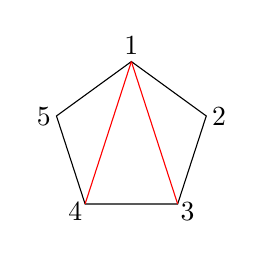
\begin{tikzpicture}
  \drawLabeledPentagon
  \draw[color=red] (P1) -- (P3);
  \draw[color=red] (P1) -- (P4);
\end{tikzpicture} 
\end{gathered} .
\end{equation}
%We can immediately see the parallels with our $\Gr(2,5)$ situation (this is an example of the more general Pl\"ucker embedding which connects $\Gr(k,n)$ with projective space). 
We can associate the line connecting points $i$ and $j$ with the Pl\"ucker coordinate $\ket{ij}$; if we further assign these lines length $\ket{ij}$, the resulting pentagon is cyclic (in the sense that all its vertices reside on a common circle) due to Ptolemy's theorem. Conversely, all cyclic $n$-gons represent a point in $\Gr_+(2,n)$~\cite{Arkani-Hamed:2014bca}. Note that the length of the three diagonals that are not present in this triangulation are determined by the length of the seven lines that are present (including edges); the problem has been reduced to geometry. This makes clear why these three diagonals---the three eliminated above---are redundant for the purpose of determining whether a matrix is in $\Gr_+(2,5)$. 

From the first relation in~\eqref{eq:plucker} we see that we could have instead chosen to check the positivity of $\ket{24}$ rather than $\ket{13}$. This corresponds to choosing a different triangulation, which we get by trading the latter diagonal for the former:
\begin{equation}
\begin{gathered}
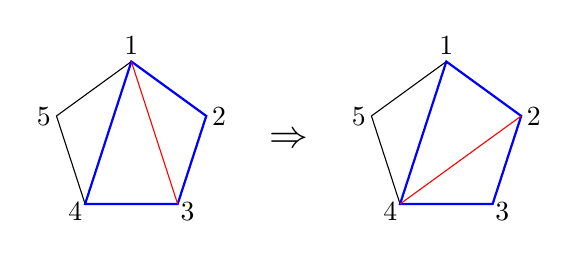
\begin{tikzpicture}
  \drawLabeledPentagon
  \draw[color=blue, thick] (P1) -- (P2) -- (P3) -- (P4) -- cycle;
  \draw[color=red] (P1) -- (P3);
  \draw (2,0) node {\scalebox{1.4}{$\Rightarrow$}};
\begin{scope}[xshift = 4cm]
  \drawLabeledPentagon
  \draw[color=blue, thick] (P1) -- (P2) -- (P3) -- (P4) -- cycle;
  \draw[color=red] (P2) -- (P4); 
\end{scope}
\end{tikzpicture}
\end{gathered}.  
\end{equation}
We have highlighted in blue the fact that both diagonals are framed by the same quadrilateral face. More generally, we can pick any quadrilateral face and flip the diagonal it contains to generate a different triangulation. Repeatedly performing these flips generates all possible triangulations of the pentagon, as can be seen in figure~\ref{fig:pent_triangulations}. Each triangulation provides a set of edges/minors whose positivity ensures that a matrix is in $\Gr_+(2,5)$. 

In an analogous way, cluster algebras answer questions about positivity for a larger class of algebraic varieties (and in particular for all $\Gr_+(k,n)$) by considering {\it clusters} that can all be generated by an operation called {\it mutation}, just as all triangulations of the pentagon are generated by flipping the diagonals of quadrilateral faces. We now turn to the definition of these objects, by first considering how the example of $\Gr_+(2,5)$ can be rephrased in terms of cluster algebras.

\begin{figure}[t]   \centering
  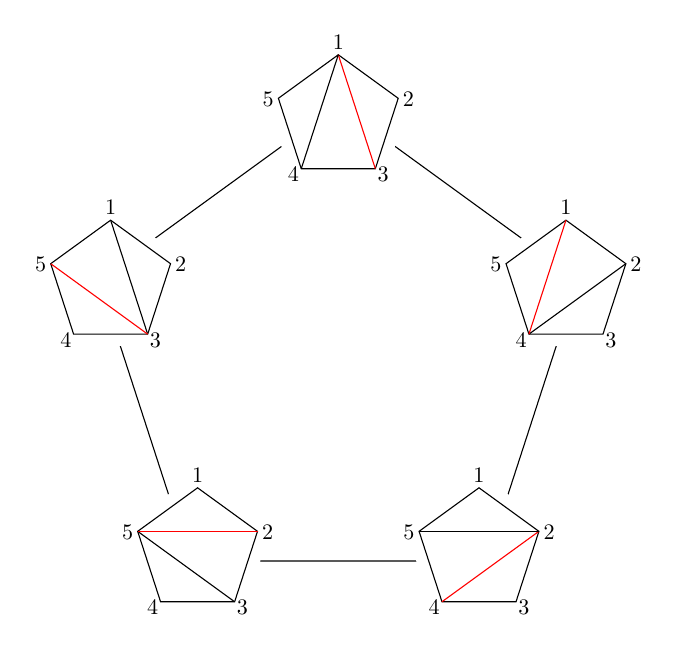
\begin{tikzpicture}[scale=0.8, every node/.style={scale=0.8}]
	\coordinate (P1) at (90:4);
	\coordinate (P2) at (18:4);
	\coordinate (P3) at (306:4);
	\coordinate (P4) at (234:4);
	\coordinate (P5) at (162:4);
	\draw (P1) -- (P2) -- (P3) -- (P4) -- (P5) -- cycle;
	\begin{scope}[shift = {(90:3.8)}]
	\drawLabeledPentagon
	\draw[color=red] (P1) -- (P3);
	\draw[color=black] (P1) -- (P4);
	\end{scope}
	\begin{scope}[shift = {(18:3.8)}]
	\drawLabeledPentagon
	\draw[color=black] (P2) -- (P4);
	\draw[color=red] (P1) -- (P4);
	\end{scope}
	\begin{scope}[shift = {(306:3.8)}]
	\drawLabeledPentagon
	\draw[color=red] (P2) -- (P4);
	\draw[color=black] (P2) -- (P5);
	\end{scope}
	\begin{scope}[shift = {(234:3.8)}]
	\drawLabeledPentagon
	\draw[color=black] (P3) -- (P5);
	\draw[color=red] (P2) -- (P5);
	\end{scope}
	\begin{scope}[shift = {(162:3.8)}]
	\drawLabeledPentagon
	\draw[color=black] (P1) -- (P3);
	\draw[color=red] (P3) -- (P5);
	\end{scope}
\end{tikzpicture}
  \caption{Mutating on the red chord moves you clockwise around the figure.}
\label{fig:pent_triangulations}
\end{figure}


\subsection{Clusters, Mutations, and Cluster ${\cal A}$-coordinates}

Clusters can be thought of as quiver diagrams---namely, oriented graphs equipped with arrows connecting different nodes---in which each node is assigned a cluster coordinate.\footnote{Here and throughout, we are implicitly restricting ourselves to skew-symmetric cluster algebras of geometric type~\cite{}.} We can form a cluster of $\Gr(2,5)$ out of our original triangulation~\eqref{eq:pent_triangulation} by assigning an orientation to the pentagon and all subtriangles, such as
\begin{equation}\label{eq:oriented-pentagon}
\begin{gathered}
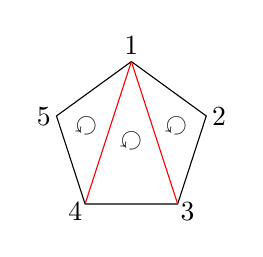
\begin{tikzpicture}
  \drawLabeledPentagon
  \draw[color=red] (P1) -- (P3);
  \draw[color=red] (P1) -- (P4);
  \draw (18:.6) node[rotate=144] {$\circlearrowleft$};
  \draw (0:0) node[rotate=144] {$\circlearrowleft$};
  \draw (162:.6) node[rotate=144] {$\circlearrowleft$};
\end{tikzpicture} 
\end{gathered} \ .
\end{equation}
The nodes of our cluster are then given by the lines of this triangulation (making the minors $\ket{ab}$ our cluster coordinates), where an arrow is assigned from $\ket{ab}$ to $\ket{cd}$ if the triangle orientations in~\eqref{eq:oriented-pentagon} have segment $(ab)$ flowing into segment $(cd)$. This gives us the quiver
\begin{equation}\label{eq:gr25-seed}
\begin{gathered}
\begin{xy} 0;<1pt,0pt>:<0pt,-1pt>::
	(25,30) *+{\langle 13\rangle} ="0",
	(75,30) *+{\langle 14\rangle} ="1",
	(125,30) *+{\framebox[5ex]{$\langle 15\rangle$}} ="2",
	(125,70) *+{\framebox[5ex]{$\langle 45\rangle$}} ="3",
	(75,70) *+{\framebox[5ex]{$\langle 34\rangle$}} ="4",
	(25,70) *+{\framebox[5ex]{$\langle 23\rangle$}} ="5",
	(0,0) *+{\framebox[5ex]{$\langle 12\rangle$}} ="6",
	(145,75) *+{},
	"0", {\ar"1"},
	"4", {\ar"0"},
	"0", {\ar"5"},
	"6", {\ar"0"},
	"1", {\ar"2"},
	"3", {\ar"1"},
	"1", {\ar"4"},
\end{xy}
\end{gathered} ,
\end{equation}
where the boxes around the $\ket{ii+1}$ indicate that they are \emph{frozen}---they can never change because they aren't in the interior of a quadrilateral face. The variables living at the frozen nodes can be thought of as parameterizing the boundary of our space, while the mutable nodes represent parameterizations of the interior. One can also draw arrows (with partial weight) connecting these frozen nodes (see, for instance,~\cite{ArkaniHamed:2012nw}), but we will not keep track of them here. 


We have now drawn our first cluster (also sometimes called a seed). The Pl\"ucker coordinates in this cluster are referred to as cluster $\a$-coordinates (sometimes also $\a$-variables), and they come in two flavors: mutable (for example, $\ket{13}$ and $\ket{14}$ above) and frozen ($\ket{ii+1}$ above). In any quiver, the information encoded by the arrows can also be represented in terms of a skew-symmetric matrix
\begin{equation}
b_{i j} = (\# \text{ of arrows}\; i \to j) - (\# \text{ of arrows}\; j \to i)
\label{eq:bijdef}
\end{equation}
called the exchange matrix (or the signed adjacency matrix).

The process of mutation, which we have described geometrically in terms of flipping diagonals, has a simple interpretation at the level of quivers. Given a quiver such as~\eqref{eq:gr25-seed}, we can choose any mutable node $k$ to mutate on (this is equivalent to picking which diagonal to flip). Mutation gives us back a new quiver in which the $\a$-coordinate $a_{k}$ has been sent to $a_{k}'$, where 
\begin{equation}
  \label{eq:a-coord-mutation}
  a_{k} a_{k}' = \prod_{i \vert b_{i k} > 0} a_{i}^{b_{i k}} + \prod_{i \vert b_{i k} < 0} a_{i}^{-b_{i k}},
\end{equation} (with the understanding that an empty product is set to one), while all other cluster $\a$-coordinates remain unchanged. The arrows connecting the nodes in this new quiver are also modified by carrying out the following operation:
\begin{itemize}
	\item for each path $i\to k \to j$, add an arrow $i\to j$,
	\item reverse all arrows on the edges incident with $k$,
	\item and remove any two-cycles (oppositely-oriented arrows) that may have formed.
\end{itemize}
This creates a new adjacency matrix $b_{ij}'$ via 
\begin{equation}
  \label{eq:b-mutation}
  b'_{i j} =
  \begin{cases}
    -b_{i j}, &\quad \text{if $k \in \lbrace i, j\rbrace$,}\\
    b_{i j}, &\quad \text{if $b_{i k} b_{k j} \leq 0$,}\\
    b_{i j} + b_{i k} b_{k j}, &\quad \text{if $b_{i k}, b_{k j} > 0$,}\\
    b_{i j} - b_{i k} b_{k j}, &\quad \text{if $b_{i k}, b_{k j} < 0$.}
  \end{cases}
\end{equation}
Mutation is an involution, so mutating on $a_k'$ will take you back to the original cluster (just as flipping the same diagonal twice will take you back to where you started). 

In terms of these ingredients, a cluster algebra can be defined to be a set of clusters that is closed under mutation. Thus, mutating on any non-frozen node of any cluster will generate a different cluster in the same cluster algebra. In practice, one therefore constructs cluster algebras by starting from a seed such as~\eqref{eq:gr25-seed}, and iteratively mutating on all available nodes until the set of clusters closes (or it becomes clear the cluster algebra is infinite). 

It is common to refer to certain cluster algebras by particularly nice representative clusters, when the mutable notes of the corresponding quiver form an oriented Dynkin diagram. For instance, the Gr(2,5) cluster algebra is often referred to as  $A_2$, since the mutable part of the seed~\eqref{eq:gr25-seed} is given by $\ket{13}\to\ket{14}$. Thus, we will often speak interchangeably of the cluster algebras for $\Gr(2,5)$ and $A_2$. This is a slight abuse of notation, as the $\Gr(2,5)$ cluster algebra corresponds specifically to the cluster algebra generated by the collection of frozen and mutable nodes in eq.~(\ref{eq:gr25-seed}), whereas an $A_2$ cluster algebra can in principle be dressed with any number of frozen nodes. We will see why this language is useful in the next section.

\subsection{Cluster \texorpdfstring{$\mathcal{X}$}{X}-coordinates}

Cluster algebras can also be formulated in terms of a different set of cluster coordinates, called Fock-Goncharov coordinates or $\x$-coordinates~\cite{FG03b}. As we will see in future sections, cluster \xcoords\ play a crucial role in connecting cluster algebras to polylogarithms and scattering amplitudes. While it is always possible to phrase results involving cluster algebras directly in terms of \acoords, \xcoords\ often allow for cluster-algebraic structure to be made more manifest. 

Clusters formed out of \xcoords\ can be directly constructed out of clusters involving \acoords. Given a quiver equipped with $\a$-coordinates and described by the exchange matrix $b_{ij}$, we can compute an $\x$-coordinate to assign to each mutable node by
\begin{equation} \label{eq:x_from_a_coordinates}
	x_i = \prod_j a_j^{b_{ij}}. 	
\end{equation} 
For example, the $\x$-coordinate cluster associated with~(\ref{eq:gr25-seed}) is formed by associating cluster \xcoords\ with all its mutable nodes, where these \xcoords\ are constructed by putting all Pl\"ucker coordinates that point to that node in the denominator, and all Pl\"ucker coordinates that are pointed to by that node in the numerator. That is, we get
\begin{equation} \label{eq:a2_x_seed}
	\frac{\ket{14}\ket{23}}{\ket{12}\ket{34}} \to \frac{\ket{15}\ket{34}}{\ket{13}\ket{45}},
\end{equation}
which takes the form of the generic $A_2$ quiver
\begin{equation} \label{def:xcoordsA2}
	x_1 \to x_2.
\end{equation}
In the pentagon-triangulation picture, these $\x$-coordinates describe overlapping quadrilaterals, for instance
\begin{equation}
\begin{gathered}
 {\hspace{-.8cm}}
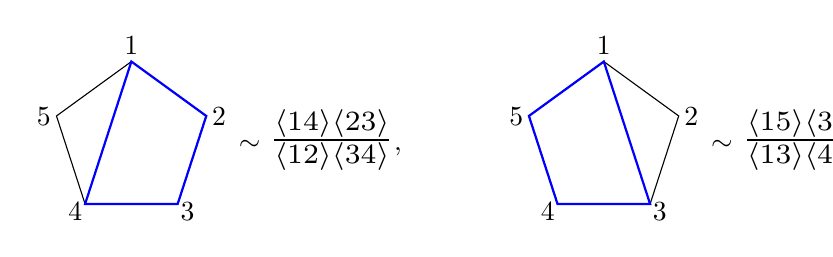
\begin{tikzpicture}
  \drawLabeledPentagon
  \draw[color=blue, thick] (P1) -- (P2) -- (P3) -- (P4) -- cycle;
  \draw (2,0) node {\hspace{.8cm}$\sim$ \scalebox{1.44}{$\frac{\ket{14}\ket{23}}{\ket{12}\ket{34}}$},}; {\hspace{1cm}}
\begin{scope}[xshift = 5cm]
  \drawLabeledPentagon
  \draw[color=blue, thick] (P1) -- (P3) -- (P4) -- (P5) -- cycle;
  \draw (2,0) node {\hspace{.8cm}$\sim$ \scalebox{1.44}{$\frac{\ket{15}\ket{34}}{\ket{13}\ket{45}}$},};
\end{scope}
\end{tikzpicture} 
\end{gathered}
\end{equation}
which come in one-to-one correspondence with the diagonals in a triangulation.

Mutation rules for \xcoords\ are different than for \acoords, and are given by
\begin{equation}
  \label{eq:x-coord-mutation}
  x_{i}' =
  \begin{cases}
    x_{k}^{-1}, &\quad i=k,\\
    x_{i} (1+x_{k}^{\sgn b_{i k}})^{b_{i k}}, &\quad i \neq k
  \end{cases}\ .
\end{equation}
Mutation still changes the arrows in the quiver diagram as it did in the case of \acoords.  Given just a quiver diagram, it can sometimes be unclear whether a given quiver should be mutated using the \acoord\ or \xcoord\ rules~\eqref{eq:a-coord-mutation} or~\eqref{eq:x-coord-mutation}. We adopt the convention in this work that if a quiver is given with no frozen nodes, it should be thought of as equipped with \xcoords.

Just as with $\a$-coordinate clusters, we can generate all $\x$-coordinate clusters by mutation. Mutating on alternating nodes of our $A_2$ cluster~\eqref{def:xcoordsA2} (starting with $x_2$), we generate the following sequence of clusters:
\begin{align}
  x_1 &\to \color{black}{x_2} \nl
  \color{black}{x_1(1+x_2)} &\leftarrow \frac{1}{x_2} \nl
  \frac{1}{x_1(1+x_2)} &\to \color{black}{\frac{x_2}{1+x_1+x_1 x_2}} \\
  \color{black}{\frac{x_1 x_2}{1+x_1}} &\leftarrow \frac{1+x_1+x_1 x_2}{x_2} \nl
  \frac{1+x_1}{x_1 x_2} &\to \color{black}{\frac{1}{x_1}} \nl
  \color{black}{x_2} &\leftarrow x_1 \nl
  &\ \ \vdots \nn
\end{align}
The series then repeats, with all arrows reversed. Note that (specifically in the case of $A_2$), if we label these $\x$-coordinates by
\begin{equation}\label{def:a2-xcoords}
  \x_1 = 1/x_1, \quad \x_2 = x_2, \quad \x_3 = x_1(1+x_2), \quad 
  \x_4 = \frac{1+x_1+x_1 x_2}{x_2}, \quad \x_5 = \frac{1+x_1}{x_1 x_2},
\end{equation}
the mutation rule in~\eqref{eq:x-coord-mutation} takes the simple form
\begin{equation}\label{eq:exchange-relation}
  1+\x_i = \x_{i-1}\x_{i+1},
\end{equation}
while all the clusters take the form $1/\x_i \to \x_{i+1}$. Eq. (\ref{eq:exchange-relation}) is commonly referred to as the $A_2$ exchange relation. 
Putting this all together, we will generically refer to an $A_2$ cluster algebra as any set of clusters $1/\x_{i-1} \to \x_i$ for $i=1\ldots5$ where the $\x_i$ satisfy eq. (\ref{eq:exchange-relation}). We believe it is useful at this point to emphasize that one can take as input any $x_1$ and $x_2$, and generate an associated $A_2$. 

A very useful feature of cluster \xcoords\ is that they come equipped with a natural Poisson bracket structure, making the Grassmannian $\Gr(k,n)$ a cluster Poisson variety~\cite{}. Namely, when two \xcoords\ appear together in a cluster of $\Gr(k,n)$, there exists a Poisson bracket that evaluates to
\begin{equation}
\{x_i, x_j \} = b_{ij} x_i x_j \ .
\end{equation}
This structure respects mutation, implying that the entry $b_{ij}$ (which counts the number of arrows from $x_i$ to $x_j$ in a given cluster's quiver) will be the same in all clusters containing both $x_i$ and $x_j$. The Poisson bracket (and associated Sklyanin bracket) will play a larger role in a forthcoming companion paper~\cite{cluster_subalgebras_ii}, so we defer further discussion of this structure to there (for existing discussions in the literature, see also~\cite{PoissonVarieties,Vergu:2015svm}).

\subsection{Subalgebras and Associahedra}\label{sec:subalgebras_associahedra}

Cluster algebras contain a rich and intricate subalgebra structure, which will play a central role in our analysis. It is simple to illustrate how these subalgebras arise by considering $\Gr(2,6)$, which triangulates the hexagon. In figure~\ref{eq:gr26-seed} we give the seed cluster for $\Gr(2,6)$ in the triangulation, \acoord, and \xcoord\ representations, respectively. Since the mutable nodes take the form of an $A_3$ Dynkin diagram, we often speak of $\Gr(2,6)$ and $A_3$ interchangeably, just as we did with $\Gr(2,5) \simeq A_2$. 

\begin{figure}
\begin{equation*}
\begin{gathered}
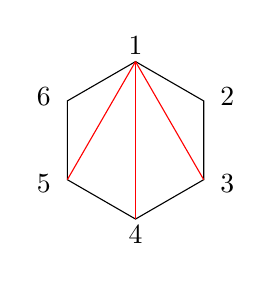
\begin{tikzpicture}
	\drawLabeledHexagon
  	\draw[color=red] (P1) -- (P3);
  	\draw[color=red] (P1) -- (P4);
  	\draw[color=red] (P1) -- (P5);
\end{tikzpicture}
\\ \scalebox{1.4}{$\Updownarrow$}
\\ \ \vspace{-1.1cm} \ \\
\begin{xy} 0;<1pt,0pt>:<0pt,-1pt>::
	(25,30) *+{\langle 13\rangle} ="0",
	(75,30) *+{\langle 14\rangle} ="1",
	(125,30) *+{\langle 15\rangle} ="2",
	(0,0) *+{\framebox[5ex]{$\langle 12\rangle$}} ="3",
	(25,70) *+{\framebox[5ex]{$\langle 23\rangle$}} ="4",
	(75,70) *+{\framebox[5ex]{$\langle 34\rangle$}} ="5",
	(125,70) *+{\framebox[5ex]{$\langle 45\rangle$}} ="6",
	(175,70) *+{\framebox[5ex]{$\langle 56\rangle$}} ="7",
	(175,30) *+{\framebox[5ex]{$\langle 16\rangle$}} ="8",
	"0", {\ar"1"},
	"1", {\ar"2"},
	"3", {\ar"0"},
	"0", {\ar"4"},
	"5", {\ar"0"},
	"1", {\ar"5"},
	"6", {\ar"1"},
	"2", {\ar"6"},
	"7", {\ar"2"},
	"2", {\ar"8"},
\end{xy} \\ 
\ \vspace{-.4cm} \ \\ 
\scalebox{1.4}{$\Updownarrow$} \\ 
\ \vspace{-.4cm} \ \\ 
\begin{xy} 0;<1pt,0pt>:<0pt,-1pt>::
	(0,0) *+\txt{\fontsize{16pt}{16pt} $\frac{\ket{14}\ket{23}}{\ket{12}\ket{34}}$} ="0",
	(75,0) *+\txt{\fontsize{16pt}{16pt} $\frac{\ket{15}\ket{34}}{\ket{13}\ket{45}}$} ="1",
	(150,0) *+\txt{\fontsize{16pt}{16pt} $\frac{\ket{16}\ket{45}}{\ket{14}\ket{56}}$} ="2",
	"0", {\ar"1"},
	"1", {\ar"2"},
\end{xy}
\end{gathered} 
\end{equation*}
\caption{One triangulation of the hexagon, and its assocated \acoord\ and \xcoord\ seed quivers.}
\label{eq:gr26-seed}
\end{figure}


The $\Gr(2,6)$ cluster algebra features 14 clusters, which can be grouped into multiple (overlapping) subalgebras. A simple example is the collection of all triangulations which involve the chord $\ket{15}$. This set contains 5 clusters and is itself a cluster algebra, which can be generated by treating $\ket{15}$ as a frozen node (or in \xcoords, freezing the node $\frac{\ket{14}\ket{56}}{\ket{16}\ket{45}}$). This of course is the cluster algebra corresponding to the triangulations of the pentagon formed by points $1,\ldots,5$, outlined here in blue:
\begin{equation}
\begin{gathered}
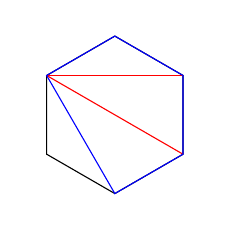
\begin{tikzpicture}
	\drawHexagon
  	\draw[color=red] (P1) -- (P3);
  	\draw[color=red] (P1) -- (P4);
	\draw[color=blue] (P1) -- (P2) -- (P3) -- (P4) -- (P5) -- cycle;
\end{tikzpicture} 
\end{gathered}
{\ ,\ }
\begin{gathered}
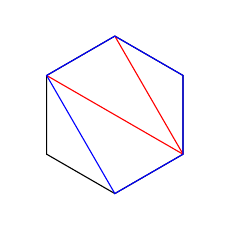
\begin{tikzpicture}
	\begin{scope}[xshift=2cm]
	\drawHexagon
  	\draw[color=red] (P2) -- (P4);
  	\draw[color=red] (P1) -- (P4);
	\draw[color=blue] (P1) -- (P2) -- (P3) -- (P4) -- (P5) -- cycle;
	\end{scope}
\end{tikzpicture} 
\end{gathered}
{\ ,\ }
\begin{gathered}
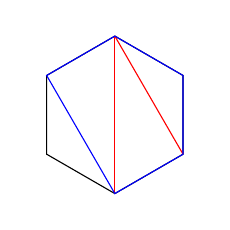
\begin{tikzpicture}
	\begin{scope}[xshift=4cm]
	\drawHexagon
  	\draw[color=red] (P2) -- (P4);
  	\draw[color=red] (P2) -- (P5);
	\draw[color=blue] (P1) -- (P2) -- (P3) -- (P4) -- (P5) -- cycle;
	\end{scope}
\end{tikzpicture} 
\end{gathered}
{\ ,\ }
\begin{gathered}
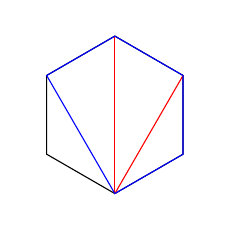
\begin{tikzpicture}
	\begin{scope}[xshift=6cm]
	\drawHexagon
  	\draw[color=red] (P2) -- (P5);
  	\draw[color=red] (P3) -- (P5);
	\draw[color=blue] (P1) -- (P2) -- (P3) -- (P4) -- (P5) -- cycle;
	\end{scope}
\end{tikzpicture} 
\end{gathered}
{\ ,\ }
\begin{gathered}
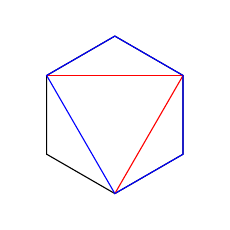
\begin{tikzpicture}
	\begin{scope}[xshift=8cm]
	\drawHexagon
  	\draw[color=red] (P1) -- (P3);
  	\draw[color=red] (P3) -- (P5);
	\draw[color=blue] (P1) -- (P2) -- (P3) -- (P4) -- (P5) -- cycle;
	\end{scope}
\end{tikzpicture}
\end{gathered}\ .
\end{equation}
We therefore refer to the collection of clusters that involve this pentagon as an $A_2$ subalgebra of $\Gr(2,6)$. 

It should be clear, upon referring back to the mutation rules~\eqref{eq:a-coord-mutation} and~\eqref{eq:x-coord-mutation}, that this $A_2$ subaglebra is truly identical to what we have been calling $\Gr(2,5)$. That is, neither the $\a$- or $\x$-coordinate mutation rule (or the rule for constructing the $\x$-coordinate cluster out of the $\a$-coordinate one) depends on nodes further than a single arrow away from the node on which one is mutating. Correspondingly, this subalgebra doesn't know about the existence of nodes involving point/column 6. (In the \xcoord\ case, the coordinate associated with the newly frozen node will change when one mutates on the node it is connected to, but the presence of this frozen node does not effect the coordinates appearing in the $A_2$ subalgebra itself.) We consider two subalgebras to be identical when the clusters they appear in only differ by nodes that have no effect on the mutable nodes of the subalgebra.  

What if we instead disallow mutation on the chord $\ket{13}$ (and the corresponding $\x$-coordinate node $\frac{\ket{12}\ket{34}}{\ket{13}\ket{24}}$)? Dropping the nodes that play no role in any of the mutations that remain gives rise to the effective quiver
\begin{equation}\label{eq:gr26-subalgebra-seed}
\begin{gathered}
\begin{xy} 0;<1pt,0pt>:<0pt,-1pt>::
	(25,0) *+{\langle 14\rangle} ="0",
	(75,0) *+{\langle 15\rangle} ="1",
	(125,0) *+{\framebox[5ex]{$\langle 15\rangle$}} ="2",
	(125,40) *+{\framebox[5ex]{$\langle 56\rangle$}} ="3",
	(75,40) *+{\framebox[5ex]{$\langle 45\rangle$}} ="4",
	(25,40) *+{\framebox[5ex]{$\langle 34\rangle$}} ="5",
	(-25,0) *+{\framebox[5ex]{$\langle 13\rangle$}} ="6",
	"0", {\ar"1"},
	"4", {\ar"0"},
	"0", {\ar"5"},
	"6", {\ar"0"},
	"1", {\ar"2"},
	"3", {\ar"1"},
	"1", {\ar"4"},
\end{xy}
\end{gathered} \ ,
\end{equation}
where we have put a box around $\ket{13}$ to make clear we are now treating it as frozen. We have also dropped the arrow from $\ket{34}$ to $\ket{13}$ since we are ignoring arrows between frozen nodes. The comparison to~\eqref{eq:gr25-seed} should be clear; this just represents a re-labeled version of $\Gr(2,5)$. 

Similarly, if we disallow mutation on the chord $\ket{14}$ (and $\frac{\ket{13}\ket{45}}{\ket{15}\ket{34}}$), we generate an $A_1 \times A_1$ subalgebra, since the chord $\ket{14}$ divides the hexagon in to two non-overlapping squares, each of which are triangulated by $A_1$ (or really $\Gr(2,4)$):
\begin{equation}
\begin{gathered}
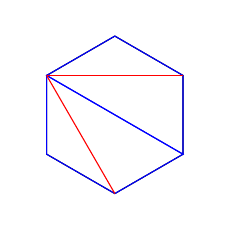
\begin{tikzpicture}
	\drawHexagon
  	\draw[color=blue] (P1) -- (P2) -- (P3) -- (P4) -- cycle;
  	\draw[color=blue] (P1) -- (P4) -- (P5) -- (P6) -- cycle;
  	\draw[color=red] (P1) -- (P5);
  	\draw[color=red] (P1) -- (P3); 
\end{tikzpicture} 
\end{gathered}
{\ ,\ }
\begin{gathered}
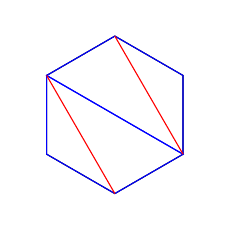
\begin{tikzpicture}
  	\begin{scope}[xshift=2cm]
	\drawHexagon
  	\draw[color=blue] (P1) -- (P2) -- (P3) -- (P4) -- cycle;
  	\draw[color=blue] (P1) -- (P4) -- (P5) -- (P6) -- cycle;
  	\draw[color=red] (P1) -- (P5);
  	\draw[color=red] (P4) -- (P2);
	\end{scope}
\end{tikzpicture} 
\end{gathered}
{\ ,\ }
\begin{gathered}
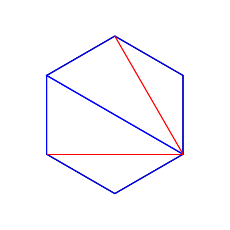
\begin{tikzpicture}
	\begin{scope}[xshift=4cm]
	\drawHexagon
  	\draw[color=blue] (P1) -- (P2) -- (P3) -- (P4) -- cycle;
  	\draw[color=blue] (P1) -- (P4) -- (P5) -- (P6) -- cycle;
  	\draw[color=red] (P6) -- (P4);
  	\draw[color=red] (P4) -- (P2);
	\end{scope}
\end{tikzpicture} 
\end{gathered}
{\ ,\ }
\begin{gathered}
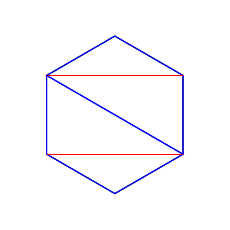
\begin{tikzpicture}
	\begin{scope}[xshift=6cm]
	\drawHexagon
  	\draw[color=blue] (P1) -- (P2) -- (P3) -- (P4) -- cycle;
  	\draw[color=blue] (P1) -- (P4) -- (P5) -- (P6) -- cycle;
  	\draw[color=red] (P6) -- (P4);
  	\draw[color=red] (P1) -- (P3);
	\end{scope}
\end{tikzpicture}
\end{gathered} \ .
\end{equation}
In appendix~\ref{appendix:subalgebras} we have tabulated the number of such $A_2$ and $A_1 \times A_1$ subalgebras in $A_3$, as well as the subalgebras of other cluster algebras that are relevant to seven-particle scattering in planar ${\cal N} = 4$. There it will be found that there are in fact six $A_2$ subalgebras and three $A_1 \times A_1$ subalgebras of $A_3$ (the remaining subalgebras do not involve the cluster in figure~\ref{eq:gr26-seed}).

This subalgebra structure can be nicely visualized by constructing an object known as the associahedron (or the Stasheff polytope) of a given cluster algebra. The vertices of this polytope each represent a cluster, while its edges represent the mutations that map these clusters into each other. For instance, figure \ref{fig:pent_triangulations} corresponds to the $\Gr(2,5) \simeq A_2$ associahedron, which also coincidentally takes the form of a pentagon. Note that every node has valency two since each cluster has two mutable vertices.

\begin{figure}[t]
  \centering
  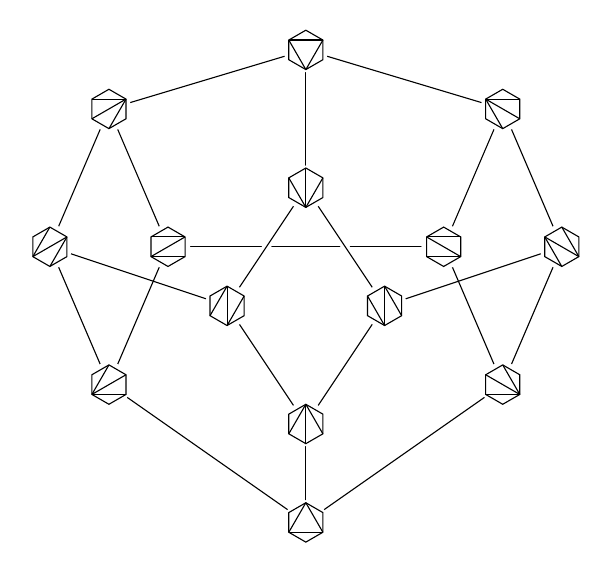
\begin{tikzpicture}[scale=2.5]
\coordinate (p1) at (0,1);
\coordinate (p2) at (1,.7);
\coordinate (p3) at (1.3,0);
\coordinate (p4) at (1,-.7);
\coordinate (p5) at (0,-1.4);
\coordinate (p6) at (-1,-.7);
\coordinate (p7) at (-1.3,0);
\coordinate (p8) at (-1,.7);
\coordinate (p9) at (-.4,-.3);
\coordinate (p10) at (0,.3);
\coordinate (p11) at (.4,-.3);
\coordinate (p12) at (0,-.9);
\coordinate (p13) at (-.7,0);
\coordinate (p14) at (.7,0);
\draw (p13) -- (p14);
\draw[color=white, line width=1mm] (p9) -- (p10);
\draw[color=white, line width=1mm] (p10) -- (p11);
\draw (p1) -- (p2) -- (p3) -- (p4) -- (p5) -- (p6) -- (p7) -- (p8) -- cycle;
\draw (p9) -- (p10) -- (p11) -- (p12) -- cycle;
\draw (p8) -- (p13) -- (p6);
\draw (p2) -- (p14) -- (p4);
\draw (p1) -- (p10);
\draw (p7) -- (p9);
\draw (p11) -- (p3);
\draw (p12) -- (p5);
\begin{scope}[shift = {(p1)}, scale=0.1, every node/.style={scale=0.5}]
	\drawHexagon
	\draw (P1) -- (P3);
	\draw (P3) -- (P5);
	\draw (P1) -- (P5);
\end{scope}
\begin{scope}[shift = {(p2)}, scale=0.1, every node/.style={scale=0.5}]
	\drawHexagon
	\draw (P1) -- (P3);
	\draw (P1) -- (P4);
	\draw (P1) -- (P5);
\end{scope}
\begin{scope}[shift = {(p3)}, scale=0.1, every node/.style={scale=0.5}]
	\drawHexagon
	\draw (P2) -- (P4);
	\draw (P1) -- (P4);
	\draw (P1) -- (P5);
\end{scope}
\begin{scope}[shift = {(p4)}, scale=0.1, every node/.style={scale=0.5}]
	\drawHexagon
	\draw (P2) -- (P4);
	\draw (P1) -- (P4);
	\draw (P6) -- (P4);
\end{scope}
\begin{scope}[shift = {(p5)}, scale=0.1, every node/.style={scale=0.5}]
	\drawHexagon
	\draw (P2) -- (P4);
	\draw (P4) -- (P6);
	\draw (P6) -- (P2);
\end{scope}
\begin{scope}[shift = {(p6)}, scale=0.1, every node/.style={scale=0.5}]
	\drawHexagon
	\draw (P2) -- (P6);
	\draw (P6) -- (P3);
	\draw (P4) -- (P6);
\end{scope}
\begin{scope}[shift = {(p7)}, scale=0.1, every node/.style={scale=0.5}]
	\drawHexagon
	\draw (P2) -- (P6);
	\draw (P3) -- (P6);
	\draw (P3) -- (P5);
\end{scope}
\begin{scope}[shift = {(p8)}, scale=0.1, every node/.style={scale=0.5}]
	\drawHexagon
	\draw (P1) -- (P3);
	\draw (P3) -- (P6);
	\draw (P3) -- (P5);
\end{scope}
\begin{scope}[shift = {(p9)}, scale=0.1, every node/.style={scale=0.5}]
	\drawHexagon
	\draw (P2) -- (P6);
	\draw (P2) -- (P5);
	\draw (P3) -- (P5);
\end{scope}
\begin{scope}[shift = {(p10)}, scale=0.1, every node/.style={scale=0.5}]
	\drawHexagon
	\draw (P1) -- (P5);
	\draw (P2) -- (P5);
	\draw (P3) -- (P5);
\end{scope}
\begin{scope}[shift = {(p11)}, scale=0.1, every node/.style={scale=0.5}]
	\drawHexagon
	\draw (P1) -- (P5);
	\draw (P2) -- (P5);
	\draw (P2) -- (P4);
\end{scope}
\begin{scope}[shift = {(p12)}, scale=0.1, every node/.style={scale=0.5}]
	\drawHexagon
	\draw (P2) -- (P6);
	\draw (P2) -- (P5);
	\draw (P2) -- (P4);
\end{scope}
\begin{scope}[shift = {(p13)}, scale=0.1, every node/.style={scale=0.5}]
	\drawHexagon
	\draw (P1) -- (P3);
	\draw (P3) -- (P6);
	\draw (P6) -- (P4);
\end{scope}
\begin{scope}[shift = {(p14)}, scale=0.1, every node/.style={scale=0.5}]
	\drawHexagon
	\draw (P1) -- (P3);
	\draw (P1) -- (P4);
	\draw (P4) -- (P6);
\end{scope}
\end{tikzpicture}
  \caption{The associahedron for $A_3\simeq\Gr(2,6)$, where each cluster is represented by a triangulation of the hexagon.}
  \label{fig:a3-poly}
\end{figure}


Similarly, the associahedron of $\Gr(2,6) \simeq A_3$ is given in figure~\ref{fig:a3-poly}. It has 14 vertices, corresponding to the 14 clusters of $\Gr(2,6)$, each with valency three. These vertices assemble into three square faces and six pentagonal faces---corresponding exactly to  the three $A_1 \times A_1$ subalgebras and the six $A_2$ subalgebras of $A_3$. This makes it easy to read off the subalgebra structure of $A_3$ directly. 

In $A_3$, it turns out that each of the faces corresponds to a distinct subalgebra. Associahedra for larger cluster algebras become quite complicated, and it is often the case that distinct faces (or higher-dimensional polytopes) correspond to identical subalgebras. As an example, the associahedron of $\Gr(4,7)\simeq E_6$, which will be the focus of much of the rest of this paper, is shown in figure~\ref{fig:e6-poly}. It has 833 vertices, each of valence 6, and 1071 pentagons corresponding to $A_2$ subalgebras; however, only 504 of these $A_2$ subalgebras are distinct.

\begin{figure}[t]  \centering
  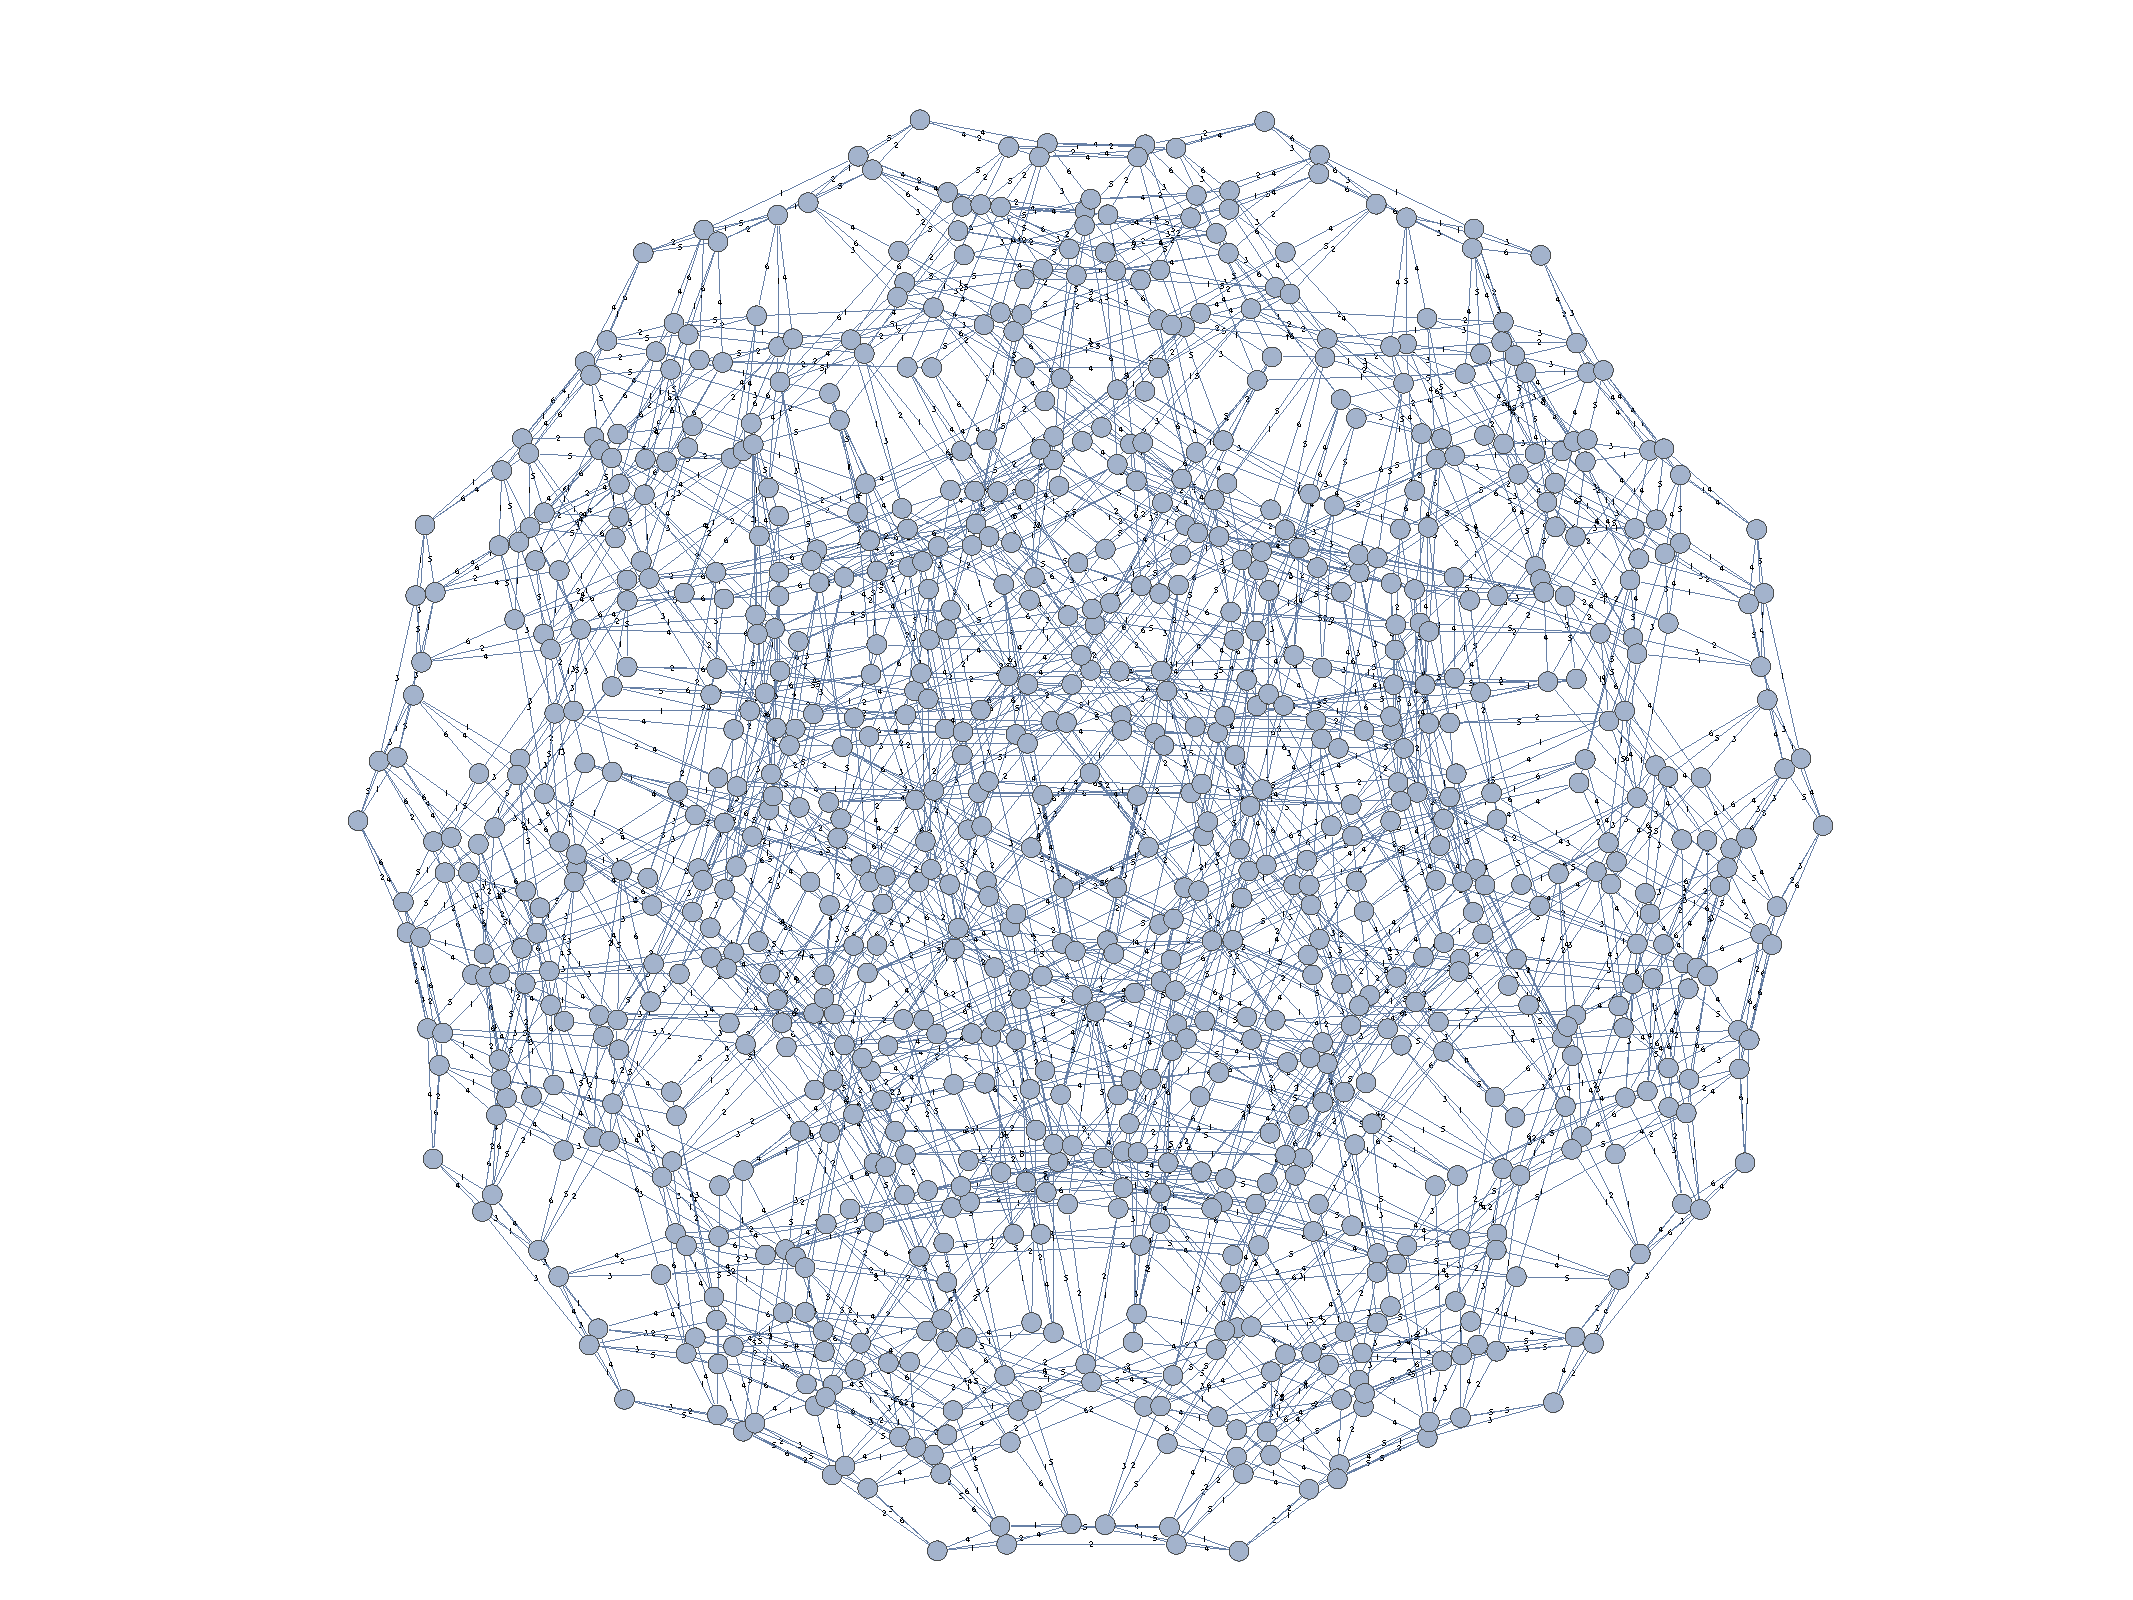
\includegraphics[scale=0.25]{e6-associahedron}
  \caption{The associahedron for $E_6\simeq\Gr(4,7)$.}
  \label{fig:e6-poly}
\end{figure}

\subsection{Grassmannian Cluster Algebras and Planar ${\cal N} = 4$ SYM }

So far we have leaned heavily on the correspondence between the triangulations of an $n$-gon and the cluster algebra for $\Gr(2,n)$. Based on the examples of $\Gr(2,5)$ and $\Gr(2,6)$, it is not hard to write down a generic seed cluster for $\Gr(2,n)$ corresponding to the triangulation consisting of all chords $\ket{13},\ldots,\ket{1n{-}1}$:
\begin{equation}\label{eq:g2n-seed}
\begin{gathered}
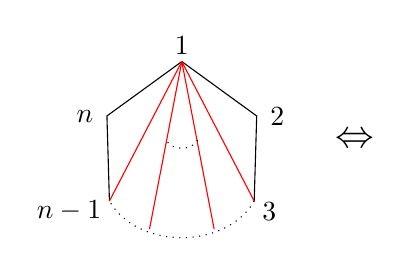
\begin{tikzpicture}
	\coordinate (P1) at (90:1);
	\coordinate (P2) at (18:1);
	\coordinate (P3) at (320:1.2);
	\coordinate (P4) at (220:1.2);
	\coordinate (P5) at (162:1);
	\draw (0,1.2) node {1};
	\draw (1,.3) node[anchor=west] {2};
	\draw (.9,-.9) node[anchor=west] {3};
	\draw (-.9,-.9) node[anchor=east] {$n-1$};
	\draw (-1,.3) node[anchor=east] {$n$};
	\draw (P1) -- (P2) -- (P3);
	\draw[dotted] (P3) to[out=240,in=300] (P4);
	\draw (P4) -- (P5) -- (P1);
	\draw[red] (P1) -- (P3);
	\draw[red] (P1) -- (P4);
	\draw[red] (P1) -- (290:1.2);
	\draw[red] (P1) -- (250:1.2);
	\draw[dotted] (.2,0) to[out=240,in=300] (-.2,0);
	\draw (2.2,0) node {\scalebox{1.4}{$\Leftrightarrow$}};
\end{tikzpicture}  
\begin{xy} 0;<1pt,0pt>:<0pt,1pt>::
	(25,40) *+{\langle 13\rangle} ="0",
	(75,40) *+{\color{white} \langle 14\rangle} ="1",
	(125,40) *+{\langle 1\ n-1 \rangle} ="2",
	(0,70) *+{\framebox[5ex]{$\langle 12\rangle$}} ="3",
	(25,0) *+{\framebox[5ex]{$\langle 23\rangle$}} ="4",
	(75,0) *+{\color{white} \framebox[5ex]{$\langle 34\rangle$}} ="5",
	(125,0) *+{\framebox[14ex]{$\langle n-2 \ n-1\rangle$}} ="6",
	(190,0) *+{\framebox[10ex]{$\langle n-1 \ n\rangle$}} ="7",
	(190,40) *+{\framebox[5ex]{$\langle 1n \rangle$}} ="8",
	(75,40) *+{\dots} ="01",
	(75,0) *+{\dots} ="05",
	"0", {\ar"1"},
	"1", {\ar"2"},
	"3", {\ar"0"},
	"0", {\ar"4"},
	"5", {\ar"0"},
	"1", {\ar"5"},
	"6", {\ar"1"},
	"2", {\ar"6"},
	"7", {\ar"2"},
	"2", {\ar"8"},
\end{xy}
\end{gathered}.
\end{equation}
Here one sees that $\Gr(2,n) \simeq A_{n-3}$. 


For $\Gr(k>2,n)$, there is no longer a simple connection with triangulations or Dynkin diagrams. However, as shown by Scott \cite{1088.22009} there exists a generalization of eq.~(\ref{eq:g2n-seed}) valid for all $\Gr(k,n)$:
\begin{equation}\label{eq:gkn-seed}
\begin{gathered}
\begin{xy} 0;<-.5pt,0pt>:<0pt,-.5pt>::
	(-100,0) *+{\framebox[10ex]{$\ket{1,\ldots,k}$}} ="-1",
	(0,0) *+{f_{1l}} ="0",
	(75,0) *+{\color{white} f_{00}} ="1",
	(150,0) *+{f_{13}} ="2",
	(225,0) *+{f_{12}} ="3",
	(300,0) *+{\framebox[5ex]{$f_{11}$}} ="4",
	(0,75) *+{f_{2l}} ="5",
	(75,75) *+{\color{white} f_{00}} ="6",
	(150,75) *+{f_{23}} ="7",
	(225,75) *+{f_{22}} ="8",
	(300,75) *+{\framebox[5ex]{$f_{21}$}} ="9",
	(0,150) *+{\color{white} f_{00}} ="10",
	(75,150) *+{\color{white} f_{00}} ="11",
	(150,150) *+{\color{white} f_{00}} ="12",
	(225,150) *+{\color{white} f_{00}} ="13",
	(300,150) *+{\color{white} f_{00}} ="14",
	(0,225) *+{\framebox[5ex]{$f_{kl}$}} ="15",
	(75,225) *+{\color{white} f_{00}} ="16",
	(150,225) *+{\framebox[5ex]{$f_{k3}$}} ="17",
	(225,225) *+{\framebox[5ex]{$f_{k2}$}} ="18",
	(300,225) *+{\framebox[5ex]{$f_{k1}$}} ="19",
	(75,0) *+{\cdots} ="01",
	(75,75) *+{\cdots} ="06",
	(0,144) *+{\vdots} ="010",
	(75,144) *+{\ddots} ="011",
	(150,144) *+{\vdots} ="012",
	(225,144) *+{\vdots} ="013",
	(300,144) *+{\vdots} ="014",
	(75,225) *+{\cdots} ="016",
	"-1", {\ar"0"},
	"0", {\ar"1"},
	"0", {\ar"5"},
	"6", {\ar"0"},
	"1", {\ar"2"},
	"2", {\ar"3"},
	"2", {\ar"7"},
	"8", {\ar"2"},
	"3", {\ar"4"},
	"3", {\ar"8"},
	"9", {\ar"3"},
	"5", {\ar"6"},
	"6", {\ar"7"},
	"7", {\ar"8"},
	"8", {\ar"9"},
	"13", {\ar"7"},
	"7", {\ar"12"},
	"8", {\ar"13"},
	"5", {\ar"10"},
	"14", {\ar"8"},
	"10", {\ar"15"},
	"12", {\ar"17"},
	"19", {\ar"13"},
	"18", {\ar"12"},
	"13", {\ar"18"},
	"17", {\ar"11"},
	"16", {\ar"10"},
	"13", {\ar"14"},
	"12", {\ar"13"},
	"11", {\ar"12"},
	"10", {\ar"11"},
	"7", {\ar"1"},
	"11", {\ar"5"},
	"12", {\ar"6"},
	"1", {\ar"6"},
	"6", {\ar"11"},
	"11", {\ar"16"},
\end{xy}
\end{gathered} ,
\end{equation}
where $l=n-k$ and 
\begin{equation}
  f_{i j} =
  \begin{cases}
    \langle i+1, \dotsc, k, k+j, \dotsc, i+j+k-1\rangle, \qquad &i \leq l-j+1,\\
    \langle 1, \dotsc, i+j-l-1, i+1, \dotsc, k, k+j, \dotsc, n\rangle, \qquad &i >l-j+1.
  \end{cases}
\end{equation}
(Note that evaluating the above expression for $k=2$ will give a rotated version of~\eqref{eq:g2n-seed} and the instances of $\Gr(2,n)$ in the previous sections.) The cluster algebra on $\Gr(k,n)$ is therefore of rank $(n-k-1)(k-1)$, i.e.~the number of mutable nodes in~\eqref{eq:gkn-seed}. 

%We have emphasized Grassmannian cluster algebras so far for two reasons: 1) the correspondence with triangulations and positive matrices make them easy to gain an intuition for and 2) the cluster algebra for $\Gr(4,n)$ is intimately connected to $n$-particle kinematics in $\mathcal{N}=4$ SYM. Let us now address point 2 a bit more in detail.

The cluster algebra on $\Gr(4,n)$ naturally appears in planar $\mathcal{N}=4$ SYM theory, where it parametrizes the space of $n$-particle kinematics. To make this connection, one first defines a set of dual coordinates $x_i$ in terms of the external momenta $p_i$ (which are endowed with a natural ordering in the planar limit) by
\begin{equation}
p_i^{\alpha \dot \alpha} = \lambda_i^\alpha \tilde \lambda_i^{\dot \alpha} = x_i^{\alpha \dot \alpha} - x_{i+1}^{\alpha \dot \alpha} \, , \label{eq:dual_coordiantes}
\end{equation}
where $x_{n+1}^{\alpha \dot \alpha} \equiv x_1^{\alpha \dot \alpha}$. These coordinates describe the cusps of a light-like Wilson loop dual to the amplitude; as a result, the original amplitude respects an additional superconformal symmetry that is associated with these dual coordinates (up to an anomaly associated with the cusps of the Wilson loop, which is accounted for by the BDS ansatz)~\cite{Bern:2005iz,Drummond:2007au,Bern:2008ap,Drummond:2008aq,Drummond:2006rz,Bern:2006ew,Bern:2007ct,Alday:2007hr,Drummond:2008vq}. In terms of the quantities in~\eqref{eq:dual_coordiantes}, we can further define momentum twistors $Z_i$
\begin{equation}
Z^R_i = (\lambda_i^\alpha, x_i^{\beta \dot \alpha} \lambda_{i \beta}) \, ,
\end{equation}
where $R = (\alpha, \dot \alpha)$ is an $SU(2,2)$ index. Momentum twistors are invariant under the little group, which acts as an overall rescaling $Z_i^R \rightarrow  t_i Z_i^R$, and as such represent points in $\mathbb{CP}^3$. 

If we assemble these momentum twistors into a $4 \times n$ matrix in which the $i^\text{th}$ column corresponds to the four $SU(2,2)$ components of $Z_i^R$, invariance under the dual conformal group becomes invariance under $\text{SL}(4)$. The overall rescaling symmetry of one of the momentum twistors can be combined with this $\text{SL}(4)$ invariance to identify this matrix as a point in the (not necessarily positive) Grassmannian $\Gr(4,n)$, modulo the rescaling invariance of the remaining $n-1$ columns. Thus, the kinematic data of an $n$-point scattering process is encoded in a momentum twistor matrix
\begin{equation}
Z_n \in \Gr(4,n)/\text{GL}(1)^{n-1}. \label{eq:gr4n_momentum_twistor}
\end{equation}
For more details regarding this correspondence, see~\cite{ArkaniHamed:2012nw,Golden:2013xva}. 

To relate the dual-conformal invariants encoded in $Z_n$ to more familiar kinematic quantities, we can translate the (cyclically ordered) Mandelstam invariants into squared differences of dual coordinates,
\begin{equation} 
s_{i,\dots,j-1} \equiv (p_i + \dots p_{j-1})^2= \text{det}(x_i^{\alpha \dot \alpha} - x_j^{\alpha \dot \alpha}) \equiv x_{ij}^2. \label{eq:mandelstam_dual_coord}
\end{equation}
Dual conformal invariants can be constructed out of these objects by putting together combinations that are invariant under the dual conformal inversion generator, which acts on these coordinates as
\begin{equation}
I( x_i^{\alpha \dot \alpha}) = \frac{x_i^{\alpha \dot \alpha}}{x_i^2}, \quad  I(x_{ij}^2) = \frac{x_{ij}^2}{x_i^2 x_j^2}.
\end{equation}
Thus, (regulated) amplitudes in this theory depend only on ratios of squared differences in which the same dual indices appear in both the numerator and denominator. The quantities $x_{ij}^2$ can be translated into momentum twistors using the relation
\begin{equation}
x_{ij}^2 = \frac{\text{det}(Z_{i-1} Z_i Z_{j-1} Z_j)}{(\epsilon_{\alpha \beta} \lambda^\alpha_{i-1} \lambda^\beta_i) (\epsilon_{\gamma \delta} \lambda^\gamma_{j-1} \lambda^\delta_j)},
\end{equation}
where $\epsilon_{\alpha \beta}$ is the Levi-Civita tensor. In dual-conformally invariant quantities, the spinor products $\epsilon_{\alpha \beta} \lambda^\alpha_{i-1} \lambda^\beta_i$ all cancel, leaving only determinants of four-tuples of momentum twistors. These are just minors of the momentum twistor matrix~\eqref{eq:gr4n_momentum_twistor}, which we recognize as the cluster \acoords  
\begin{equation}
\ket{i j k l} = \text{det}(Z_i Z_j Z_k Z_l).
\end{equation}
Note that the two-particle Mandelstams $s_{i,i+1}$ correspond to the frozen nodes of~\eqref{eq:gkn-seed}, while higher-particle Mandelstams and more general (polynomials of) Pl\"ucker coordinates can appear as mutable nodes.

By construction, the \xcoords\ on $\Gr(4,n)$ derived from the seed~\eqref{eq:gkn-seed} respect dual-conformal invariance. Both mutation rules~\eqref{eq:a-coord-mutation} and~\eqref{eq:x-coord-mutation} preserve this property (and commute with the translation~\eqref{eq:x_from_a_coordinates}), ensuring that all \xcoords\ are dual conformal invariants. Such invariants cannot be formed in four- or five-particle kinematics, due to an insufficient number of non-lightlike separated points (since we are in massless kinematics, $x_{ii+1}^2 = 0$ for all $i$). This fact shows up in the seed~\eqref{eq:gkn-seed} as $\Gr(4,n<6)$ having no mutable nodes (and therefore no \xcoords). For $n>5$, there are $3(n-5)$ mutable nodes in $\Gr(4,n)$, matching the number of algebraically independent dual conformal invariants that can be formed out of $n$ massless particles~\cite{}. %For more than six particles, this is fewer than the number of multiplicatively independent dual conformal invariants due to . , $n(n-3)/2$. 

\begin{figure}[t]
\centering
\begin{subfigure}[b]{0.45\textwidth}
\begin{equation*}
\begin{gathered}
\begin{xy} 0;<-.5pt,0pt>:<0pt,-.5pt>::
         (-100,0) *+{\framebox[7ex]{$\ket{1234}$}} ="0",
	(0,0) *+{\ket{2346}} ="1",
	(100,0) *+{\framebox[7ex]{$\ket{2345}$}} ="2",
	(0,75) *+{\ket{1346}} ="3",
	(100,75) *+{\framebox[7ex]{$\ket{3456}$}} ="4",
	(0,150) *+{\ket{1246}} ="5",
	(100,150) *+{\framebox[7ex]{$\ket{1456}$}} ="6",
	(0,225) *+{\framebox[7ex]{$\ket{1236}$}} ="7",
	(100,225) *+{\framebox[7ex]{$\ket{1256}$}} ="8",
	"0", {\ar"1"},
	"1", {\ar"2"},
	"3", {\ar"4"},
	"5", {\ar"6"},
	"1", {\ar"3"},
	"3", {\ar"5"},
	"5", {\ar"7"},
	"4", {\ar"1"},
	"6", {\ar"3"},
	"8", {\ar"5"},
\end{xy}
\end{gathered} 
\end{equation*}
\caption{} \label{fig:g46-a-seed}
\end{subfigure}
\hspace*{\fill} 
\begin{subfigure}[b]{0.45\textwidth}
\begin{equation*}
\begin{gathered}
\begin{xy} 0;<-.5pt,0pt>:<0pt,-.5pt>::
	(0,0) *+\txt{\fontsize{16pt}{16pt} $\frac{\ket{2345}\ket{1346}}{\ket{1234}\ket{3456}}$} ="1",
	(0,100) *+\txt{\fontsize{16pt}{16pt} $\frac{\ket{3456}\ket{1246}}{\ket{2346}\ket{1456}}$} ="3",
	(0,200) *+\txt{\fontsize{16pt}{16pt} $\frac{\ket{1456}\ket{1236}}{\ket{1346}\ket{1256}}$} ="5",
	"1", {\ar"3"},
	"3", {\ar"5"},
\end{xy}
\end{gathered} 
\end{equation*}
\caption{} \label{fig:g46-x-seed}
\end{subfigure}
\caption{The \acoord\ seed quiver (a) and \xcoord\ seed quiver (b) for $\Gr(4,6)$.} 
\label{fig:g46-seed}
\end{figure}

The \acoord\ and \xcoord\ seed clusters of the first nontrivial example, $\Gr(4,6)$, are shown in figure~\ref{fig:g46-seed}. As discussed above, the three \xcoords\ in this cluster furnish us with a chart that covers the space of (dual-conformally invariant) six-particle kinematics. Moreover, we can generate new charts by mutation---every \xcoord\ cluster of $\Gr(4,n)$ provides a valid chart for $n$-particle kinematics. As explored in great depth in~\cite{ArkaniHamed:2012nw}, these charts are especially well suited to describing the boundaries of the positive Grassmannian $\Gr_+(4,n)$, where the integrands of $n$-particle amplitudes can develop physical singularities. In particular, every such boundary occurs at the vanishing locus of an \acoord\ of $\Gr(4,n)$, which implies it also occurs at the vanishing locus of some set of \xcoords.  

This fact is especially propitious for loop-level amplitudes (and integrals) that only have branch points on the boundaries of the positive Grassmannian. In such cases, the symbol alphabet encoding the polylogarithmic part of these amplitudes is naturally given in terms of cluster coordinates. We defer discussion of the coaction and symbol alphabets to section~\ref{sec:coproduct}, but here note that it is multiplicative independence, rather than algebraic independence, that is relevant in the context of symbol alphabets. Thus, while it is not possible to realize all boundaries of the positive Grassmannian as the vanishing loci of either type of cluster coordinate in a single chart~\cite{ArkaniHamed:2012nw}, all boundaries are exposed as the vanishing of some symbol letter if cluster \acoords\ or \xcoords\ on $\Gr(4,n)$ are adopted as a symbol alphabet.

While amplitudes in planar ${\cal N}=4$ are not generically expected to have this property (and indeed, certain Feynman integrals have been computed that do not~\cite{Bourjaily:2018aeq,Henn:2018cdp}), an infinite class of amplitudes do---namely, all two-loop MHV amplitudes~\cite{CaronHuot:2011ky}, and all six- and seven-particle amplitudes computed to date~\cite{CaronHuot:2011kk,Dixon:2014iba,Drummond:2014ffa,Dixon:2015iva,Caron-Huot:2016owq,Dixon:2016nkn}. The significance of this property is illustrated by the two-loop, six-particle remainder function, which encodes the MHV amplitude. Namely, this function can be put in the form
\begin{equation} \label{eq:R26cobracket}
	R^{(2)}_6 = \sum_{\text{cyclic}} \left[ \text{Li}_4\left(-\frac{\langle 2345 \rangle \langle 1346 \rangle}{\langle 1234 \rangle \langle 3456 \rangle}\right) - \frac{1}{4} \text{Li}_4 \left(-\frac{\langle 1246 \rangle \langle 1345 \rangle}{\langle 1234 \rangle \langle 1456 \rangle}\right) \right] + \dots,
%	R^{(2)}_6 \stackrel{\delta}{=} \sum_{\text{cyclic}} \left[ \text{Li}_4\left(-\frac{\langle 1234 \rangle \langle 2356 \rangle}{\langle 1236 \rangle \langle 2345 \rangle}\right) - \frac{1}{4} \text{Li}_4 \left(-\frac{\langle 1246 \rangle \langle 1345 \rangle}{\langle 1234 \rangle \langle 1456 \rangle}\right) \right],
\end{equation}
\draftnote{check normalization} where the cyclic sum is over all rotations of the four-bracket indices $i \rightarrow i+j$ for $0\leq j <6$, and the dots indicate this equality only holds up to products of lower-weight polylogarithms. This projection is well-defined and will be introduced, along with the $n$-particle remainder function, in section~\ref{sec:cluster_polylog_MHV_review}. Here we just emphasize the simplicity of this expression, which takes the form of classical polylogarithms with negative \xcoord\ arguments. (In particular, the argument of the first polylogarithm appears in figure~\ref{fig:g46-x-seed}, while the argument of the second polylogarithm appears after mutating on the top node of this cluster.) Moreover, the part of the expression we have dropped in~\eqref{eq:R26cobracket} can also expressed entirely in terms of products of classical polylogarithms with negative \xcoord\ arguments~\cite{Golden:2014xqf}. 

This surprising property---of being expressible as polylogarithms with negative \xcoord\ arguments---is enjoyed by the remainder function at all $n$. However, for $n>6$ the remainder function has a nonclassical component, so generalized polylogarithms (in addition to classical polylogarithms) with negative \xcoord\ arguments also appear~\cite{}. Although this component represents the mathematically most complicated part of the remainder function, it was shown in~\cite{Golden:2014xqa} that it is decomposable into building blocks related to the $A_2$ and $A_3$ subalgebras of $\Gr(4,n)$. This allows the all-$n$ symbol computed in~\cite{CaronHuot:2011ky} to be systematically upgraded to a function, as was done for seven particles in~\cite{Golden:2014xqf}. In the later sections of this paper, we demonstrate the existence of further subalgebra structure in the nonclassical part of the seven-particle remainder function (we leave consideration of higher-point kinematics to future work~\cite{cluster_subalgebras_ii}). The \acoord\ and \xcoord\ seeds for $\Gr(4,7)$ are presented in figure~\ref{fig:g47-seed}.

Before turning to the remaining aspects of cluster algebras that we wish to develop, we note that plabic graphs---which are dual to the clusters we've been describing---encode a great deal more about planar ${\cal N}=4$ than we have had reason to touch on. In particular, \draftnote{boundaries---a subset of which are our subalgebras (?)}. We refer interested readers to the exposition of this rich structure given in~\cite{ArkaniHamed:2012nw}.

\begin{figure}
\centering
\begin{subfigure}[b]{0.45\textwidth}
\begin{equation*}
\begin{gathered}
\begin{xy} 0;<-.5pt,0pt>:<0pt,-.5pt>::
         (-100,0) *+{\framebox[7ex]{$\ket{1234}$}} ="0",
	(0,0) *+{\ket{2347}} ="1",
	(100,0) *+{\ket{2346}} ="2",
	(200,0) *+{\framebox[7ex]{$\ket{2345}$}} ="3",
	(0,75) *+{\ket{1347}} ="4",
	(100,75) *+{\ket{3467}} ="5",
	(200,75) *+{\framebox[7ex]{$\ket{3456}$}} ="6",
	(0,150) *+{\ket{1247}} ="7",
	(100,150) *+{\ket{1467}} ="8",
	(200,150) *+{\framebox[7ex]{$\ket{4567}$}} ="9",
	(0,225) *+{\framebox[7ex]{$\ket{1237}$}} ="10",
	(100,225) *+{\framebox[7ex]{$\ket{1267}$}} ="11",
	(200,225) *+{\framebox[7ex]{$\ket{1567}$}} ="12",
	"0", {\ar"1"},
	"1", {\ar"2"},
	"2", {\ar"3"},
	"4", {\ar"5"},
	"5", {\ar"6"},
	"7", {\ar"8"},
	"8", {\ar"9"},
	"1", {\ar"4"},
	"2", {\ar"5"},
	"4", {\ar"7"},
	"5", {\ar"8"},
	"7", {\ar"10"},
	"8", {\ar"11"},
	"5", {\ar"1"},
	"6", {\ar"2"},
	"8", {\ar"4"},
	"9", {\ar"5"},
	"11", {\ar"7"},
	"12", {\ar"8"},
\end{xy}
\end{gathered} 
\end{equation*} 
\caption{} \label{fig:g47-a-seed}
\end{subfigure}
\hspace*{\fill} 
\begin{subfigure}[b]{0.45\textwidth}
\begin{equation*}
\begin{gathered}
\begin{xy} 0;<-.5pt,0pt>:<0pt,-.5pt>::
	(0,0) *+\txt{\fontsize{16pt}{16pt} $\frac{\ket{2346}\ket{1347}}{\ket{1234}\ket{3467}}$} ="1",
	(220,0) *+\txt{\fontsize{16pt}{16pt} $\frac{\ket{2345}\ket{3467}}{\ket{2347}\ket{3456}}$} ="2",
	(0,100) *+\txt{\fontsize{16pt}{16pt} $\frac{\ket{3467}\ket{1247}}{\ket{2347}\ket{1467}}$} ="4",
	(220,100) *+\txt{\fontsize{16pt}{16pt} $\frac{\ket{2347}\ket{1467}\ket{3456}}{\ket{2346}\ket{1347}\ket{4567}}$} ="5",
	(0,200) *+\txt{\fontsize{16pt}{16pt} $\frac{\ket{1467}\ket{1237}}{\ket{1347}\ket{1267}}$} ="7",
	(220,200) *+\txt{\fontsize{16pt}{16pt} $\frac{\ket{1347}\ket{4567}\ket{1267}}{\ket{3467}\ket{1247}\ket{1567}}$} ="8",
	"1", {\ar"2"},
	"4", {\ar"5"},
	"7", {\ar"8"},
	"1", {\ar"4"},
	"2", {\ar"5"},
	"4", {\ar"7"},
	"5", {\ar"8"},
	"5", {\ar"1"},
	"8", {\ar"4"},
\end{xy}
\end{gathered} 
\end{equation*} 
\caption{} \label{fig:g47-x-seed}
\end{subfigure}
\caption{The \acoord\ seed quiver (a) and \xcoord\ seed quiver (b) for $\Gr(4,7)$.} 
\label{fig:g47-seed}
\end{figure}


%We will go in to much further detail on the connections between cluster algebras and $\mathcal{N}$=4 SYM in future sections. However, for now we will elaborate on the connections between cluster algebras and polylogarithms. For this we do not need to constrain ourselves to Grassmannian cluster algebras, and so for the next few sections we will work with the slightly more abstact language of quivers of generic \xcoords, i.e. $x_1 \to x_2$. 


\subsection{Finite Cluster Algebras}\label{sec:finite-algebras}

The procedure of writing down an oriented oriented quiver, dressing it with coordinates, and iteratively mutating on all non-frozen nodes using either the $\a$-coordinate or $\x$-coordinate mutation rule will always produce a cluster algebra. However, generic quivers give rise to exceedingly complicated cluster algebras---in fact, for a wide class of seeds, mutation will generate an infinite numbers of clusters. For the rest of this paper we will restrict our attention to finite cluster algebras, leaving the discussion of infinite algebras to a forthcoming companion paper~\cite{cluster_subalgebras_ii} (see~\cite{} for discussions of infinite cluster algebras elsewhere in the literature). 

%\footnote{There is a further distinction in the infinite case between cluster algebras which contain a finite number of quiver types (dressed in an infinite number of ways with distinct cluster coordinates), and those which contain infinitely many quivers as well as coordinates.} 

Fortunately, Fomin and Zelevinksy classified all finite cluster algebras in \cite{1054.17024}. In particular, they showed that a cluster algebra is of finite type if and only if the mutable part of at least one of its clusters takes the form of an oriented, simply-laced Dynkin diagram: $A_n$, $D_n$, or $E_{n\le8}$.  As we will primarily be interested in subalgebras of the cluster algebra on $\Gr(4,7)$, we here focus on the cases where $n < 6$ (and on the case of $E_6 \simeq \Gr(4,7)$ itself). 

As mentioned above, cluster algebras of type $A_n$ can be generated by the seed
\begin{equation}\label{def:An}
  x_1\to x_2\to \ldots \to x_n \ ,
\end{equation}
which corresponds to the cluster algebra on $\Gr(2,n{+}3)$. Each of the clusters in these algebras can be though as triangulating an $(n+3)$-gon, where the \acoords\ correspond to chords and the \xcoords\ to quadrilateral faces. This makes the counting easy: the number of clusters for $A_n$ is given by the Catalan number $C(n+1)$, the number of distinct \acoords\ is $\binom{n+3}{2}-n$, and the number of distinct \xcoords\ is $2\binom{n+3}{4}$. Any smaller polygon embedded into the $(n+3)$-gon gives rise to a subalgebra; for example, there are $56=\binom{8}{5}$ pentagonal embeddings in an octagon, so there are 56 $A_2$ subalgebras in $A_5$. 

Of particular interest is the cluster algebra generated by $A_3 \simeq \Gr(4,6)$, which describes six-particle scattering. By comparison with figure~\ref{fig:g46-x-seed}, we see that the \xcoords\ in the quiver~\eqref{def:An} act as coordinates on the space of momentum twistors, where they correspond to the functions
\begin{equation}\label{eq:a3-seed-def}
x_1 = \frac{\ket{2345}\ket{1346}}{\ket{1234}\ket{3456}}, \quad x_2 = \frac{\ket{3456}\ket{1246}}{\ket{2346}\ket{1456}}, \quad x_3 = \frac{\ket{1456}\ket{1236}}{\ket{1346}\ket{1256}}.
\end{equation}
More generally, any \acoord\ in $\Gr(4,6)$ can be expressed in terms of the variables $x_1$, $x_2$, and $x_3$ by evaluation on the momentum twistor matrix
\begin{equation} \label{eq:a3_momentum_twistor_matrix}
Z_{A_3} = 
\begingroup
\setlength\arraycolsep{4pt}
\begin{pmatrix} 
1 & 1 & 0 & 0 & x_2 x_3 & 0 \\
0 & 1 & 1+x_3 & x_3 & 0 & 0 \\
1+x_1 & x_1 & 0 & 0 & 0 & -1 \\
0 & 0 & 1 & 1 & 1 & 0
\end{pmatrix}.
\endgroup 
\end{equation}
The chief advantage of working directly in terms of cluster \xcoords\ such as $x_1$, $x_2$, and $x_3$ is that they trivialize all Pl\"ucker relations~\eqref{eq:plucker-rel}. Furthermore, cluster coordinates rationalize many of the square roots that appear when amplitudes and integrals are expressed in terms of dual conformally invariant cross ratios~\cite{Bourjaily:2018aeq}. For instance, in this chart the dual conformal cross ratios commonly used to express the six-particle amplitude evaluate to
\begin{align} \label{eq:uvw_in_x}
u &= \frac{\ket{6123}\ket{3456}}{\ket{6134}\ket{2356}} = \frac{x_2 x_3}{1+x_3+x_2 x_3}, \\ 
v &= \frac{\ket{1234} \ket{4561}}{\ket{1245}\ket{3461}} =\frac{1}{1+x_2+x_1 x_2}, \\ 
w &= \frac{\ket{2345} \ket{5612}}{\ket{2356}\ket{4512}} =\frac{x_1 x_2}{(1+x_2+x_1 x_2)(1+x_3+x_2 x_3)},
\end{align}
which rationalizes the square root that appears in six-particle kinematics 
\begin{equation}
\sqrt{(1 - u - v - w)^2 - 4 u v w} = \frac{x_2 (1 - x_1 x_3)}{(1 + x_2 + x_1 x_2)(1 + x_3 + x_2 x_3)} .
\end{equation}
Note that the cluster coordinate expressions~\eqref{eq:uvw_in_x} are rotated compared to those given elsewhere in the literature~\cite{Golden:2013xva,Parker:2015cia} even though both arise from a seed of the form~\eqref{def:An}; this reflects a differing convention for the seed of $\Gr(k,n)$.

The first nondegenerate Dynkin diagram of type $D_n$ is $D_4$, corresponding to the seed quiver
\begin{equation} \label{eq:D4_quiver}
    \begin{gathered}
    \begin{xy} 0;<1pt,0pt>:<0pt,-1pt>::
      (0,20) *+{x_1} ="1",
      (30,20) *+{x_2} ="2",
      (60,0) *+{x_3} ="3",
      (60,40) *+{x_4} ="4",
      "1", {\ar"2"},
      "2", {\ar"3"},
      "2", {\ar"4"},
    \end{xy}
    \end{gathered} .
\end{equation}
Note here that we no longer are treating $x_1, x_2, x_3$ as defined in eq.~(\ref{eq:a3-seed-def}), the $x_i$ in eq.~(\ref{eq:D4_quiver}) are all generic variables. This seed turns out to generate the same cluster algebra as $\Gr(3,6)$; in particular, starting from the seed in~\eqref{eq:gkn-seed} and mutating on the nodes initially labeled by $f_{13}$ and then $f_{23}$, one arrives at the \xcoord\ quiver~\eqref{eq:D4_quiver}, where
\begin{equation}\label{eq:d4-seed-def}
x_1 = \frac{\ket{234}\ket{135}}{\ket{123}\ket{345}}, \quad x_2 = \frac{\ket{125}\ket{356}}{\ket{156}\ket{235}}, \quad x_3 = \frac{\ket{156}\ket{345}}{\ket{135}\ket{456}}, \quad x_4 = \frac{\ket{123}\ket{156}}{\ket{126}\ket{135}}.
\end{equation}
The corresponding momentum twistor matrix is given by
\begin{equation}
Z_{D_4} = 
\begingroup
\setlength\arraycolsep{4pt}
\begin{pmatrix} 
 x_1 & 1 & 0 & -1 & 0 & x_1 x_2 x_4 \\
 0 & -1 & 0 & 1+x_1 & x_1 (1+x_4) & x_1 (1+x_4) \\
 x_1 x_3 & x_3 (1+x_2)  & 1 & 1 & 0 & 0
 \end{pmatrix}
\endgroup .
\end{equation}
Conversely, the cluster algebra generated by $D_5$,
\begin{equation}\label{def:D5}
    \begin{gathered}
    \begin{xy} 0;<1pt,0pt>:<0pt,-1pt>::
      (0,20) *+{x_1} ="1",
      (30,20) *+{x_2} ="2",
      (60,20) *+{x_3} ="3",
      (90,0) *+{x_4} ="4",
      (90,40) *+{x_5} ="5",
      "1", {\ar"2"},
      "2", {\ar"3"},
      "3", {\ar"4"},
      "3", {\ar"5"},
    \end{xy}
    \end{gathered} ,
\end{equation}
is not equivalent to the cluster algebra on any Grassmannian (once again, ignore the notational overlap with eq.~(\ref{eq:d4-seed-def}) and treat all of the $x_i$ as generic variables). However, it appears as a subalgebra of any $\Gr(k,n)$ with rank greater than five. The $D_4$ cluster algebra consists of 50 clusters, 16 \acoords, and 104 \xcoords, while $D_5$ has 182 clusters, 25 \acoords, and 260 \xcoords. 

Finally, the cluster algebra $E_6$ is generated by the quiver
\begin{equation}\label{def:E6}
    \begin{gathered}
    \begin{xy} 0;<1pt,0pt>:<0pt,-1pt>::
      (0,0) *+{x_1} ="1",
      (30,0) *+{x_2} ="2",
      (60,0) *+{x_3} ="3",
      (60,-25) *+{x_4} ="4",
      (90,0) *+{x_5} ="5",
      (120,0) *+{x_6} ="6",
      "1", {\ar"2"},
      "2", {\ar"3"},
      "3", {\ar"4"},
      "5", {\ar"3"},
      "6", {\ar"5"},
    \end{xy}
    \end{gathered} .
\end{equation}
This cluster algebra is equivalent to $\Gr(4,7)$, as can be seen by mutating the seed~\eqref{eq:gkn-seed} on nodes $f_{12}$, $f_{13}$, $f_{23}$, $f_{12}$, $f_{22}$, and then $f_{32}$. By comparison with~\eqref{def:E6}, we then have 
\begin{align} \label{eq:E6_x_def}
x_1 &= \frac{\ket{1237} \ket{1246}}{\ket{1234}\ket{1267}}, \hspace{13.03ex} \quad \quad x_2 = - \frac{\ket{4(12)(35)(67)}}{\ket{1247} \ket{3456}}, \quad \nonumber \\
x_3 &= \frac{\ket{1245} \ket{1267} \ket{3456}}{\ket{1246} \ket{5(12)(34)(67)}}, \hspace{4.12ex} \quad \quad x_4 = -\frac{\ket{1234} \ket{4567}}{\ket{4(12)(35)(67)}}, \quad \\
 x_5 &= -\frac{\ket{1567}\ket{4(12)(35)(67)}}{\ket{1267} \ket{1345}\ket{4567}}, \quad \quad \quad x_6 = \frac{\ket{5(12)(34)(67)}}{\ket{1567}\ket{2345}}, \quad \nonumber
\end{align}
where we have made use of the notation
\begin{equation} \label{eq:twistor_intersection}
\ket{a(bc)(de)(fg)} \equiv \ket{abde}\ket{acfg}-\ket{abfg}\ket{acde}.
\end{equation}
Any \acoord\ on $\Gr(4,7)$ can be expressed in terms of these \xcoords\ using the momentum twistor matrix 
\begin{equation}
Z_{E_6} = 
\begingroup
\setlength\arraycolsep{3pt}
\begin{pmatrix} 
 -x_2 & 0 & -(1+x_4) & 0 & -x_2 & 1+x_{5,6} & (1+x_2) (1+x_{5,6}) \\
 1+x_{4,3,5} & 1 & x_3 x_4 x_5 x_6 & 0 & x_3 x_5 x_6 (1+x_2) & x_5 x_6 & -x_4 x_5 x_6 \\
 0 & 0 & x_3 x_4 & 0 & x_2 x_3 & 1 & 1 \\
 0 & 0 & -x_1 x_3 x_4 & 1 & 1+x_{3,2} & 1 & 0 \\
\end{pmatrix} ,
\endgroup
\end{equation}
where we have introduced the notation
\begin{equation} \label{eq:compound_x_def}
	x_{i_1,\ldots, i_k} = \sum_{a=1}^k \prod_{b=1}^a x_{i_b} = x_{i_1}+x_{i_1}x_{i_2} + \ldots + x_{i_1}\cdots x_{i_k}.
\end{equation}
The associahedron of $\Gr(4,7) \simeq E_6$ was displayed in figure~\ref{fig:e6-poly}; it contains 833 clusters, 42 \acoords, and 770 \xcoords. The subalgebras of $E_6$, as well as those of its subalgebras, are tabulated in appendix~\ref{appendix:subalgebras}.

%\begin{equation}
%\begin{tabular}{ c|c|c|c|c|c} 
 %$A_2$ & $A_3$ & $A_4$ & $D_4$ & $A_5$ & $D_5$ \\ 
% \hline
%504 & 364 & 98 & 35 & 7 & 14
%\end{tabular}.
%\end{equation}

\subsection{Cluster Automorphisms}\label{sec:automorphisms}

Cluster algebras come equipped with an automorphism group that maps the set of cluster coordinates (but not necessarily the set of clusters) back to itself. We introduce here only what we need to elucidate the automorphisms of the cluster algebras introduced in the last section, and refer the interested reader to~\cite{Chang:2015} for a more thorough mathematical introduction. Note that we describe automorphisms in terms of \xcoords, whereas~\cite{Chang:2015} works in the \acoord\ language. 

The simplest example of a cluster automorphism is what we call a direct automorphism. Let $\a$ be a cluster algebra equipped with a mutation rule $\mu(x_i, \bf{x})$ that mutates the cluster $\bf{x}$ on node $x_i$. Then, we can define:
\begin{quote}
{\bf Direct Automorphism}: The map $f: \a \to \a$ is a direct automorphism of $\a$ if 
\vspace{-.2cm}
 \begin{itemize}
 \item[(i)] for every cluster $\mathbf{x}$ of $\a$, $f(\mathbf{x})$ is also a cluster of $\a$, 
 \item[(ii)] $f$ respects mutations, i.e. $f(\mu(x_i,\mathbf{x})) = \mu(f(x_i),f(\mathbf{x}))$.
 \end{itemize}
\end{quote}
An example of a direct automorphism on $A_2$ is given by
\begin{equation}
  \sigma_{A_2}:\quad \mathcal{X}_i \to \mathcal{X}_{i+1},
\end{equation}
where we are using the coordinates introduced in ~\eqref{def:a2-xcoords}. This automorphism cycles the five clusters $1/\x_i\to \x_{i+1}$ amongst themselves. The action of this automorphism can also be recast as
\begin{equation}
  \sigma_{A_2}:\quad x_1\to \frac{1}{x_2},~~ x_2\to x_1(1+x_2),
\end{equation}
using the \xcoords\ $x_1$ and $x_2$ that appear in~\eqref{def:An}. 

Cluster algebras are also endowed with what we call indirect automorphisms, which respect mutations but do not map the set of clusters back to itself. Instead, indirect automorphisms map the clusters in $\a$ to clusters in $\a'$, where $\a'$ is constructed from $\a$ by multiplicatively inverting all cluster \xcoords\ and reversing the direction of all quiver arrows. Then we have:
\begin{quote}
{\bf Indirect Automorphism}: The map $f: \a \to \a'$ is an indirect automorphism if 
\vspace{-.2cm}
\begin{itemize}
  \item[(i)] for every cluster $\mathbf{x}$ of $\a$, $f(\mathbf{x})$ is a cluster of $\a'$ 
  \item[(ii)] $f$ respects mutations, i.e. $f(\mu(x_i,\mathbf{x})) = \mu(f(x_i),f(\mathbf{x}))$.
\end{itemize}
\end{quote}
$A_2$ is also equipped with an indirect automorphism generated by
\begin{equation}
  \tau_{A_2}:\quad \mathcal{X}_i \to \mathcal{X}_{6-i},
\end{equation}
where indices are understood to be mod 5. This can be recast in term of $x_1$ and $x_2$ as
\begin{equation}
  \tau_{A_2}:\quad x_1 \to \frac{1}{x_2}, ~~x_2 \to \frac{1}{x_1}.
\end{equation}
To see that this is an indirect automorphism, consider
\begin{align}
  \tau_{A_2}(1/\x_1 \to \x_2) =&~1/\x_5 \to \x_4 \ .
\end{align}
Inverting the cluster coordinates on the right hand side and reversing the arrow, we get back to $\x_5 \leftarrow 1/\x_4$, which was one of the original clusters of $A_2$. It is useful to think of indirect automorphisms as generating a ``mirror'' or ``flipped'' version of the original cluster algebra, where the total collection of $\x$-coordinates is the same, but their Poisson bracket has flipped sign. The existence of this flip then can be seen as resulting from the arbitrary choice of overall sign for the exchange matrix; picking the other sign would have generated the same cluster-algebraic structure, but with different labels for the nodes. Indirect automorphisms capture the superficiality of this notation change.

The automorphisms $\sigma_{A_2}$ and $\tau_{A_2}$ generate the complete automorphism group for $A_2$, namely the dihedral group $D_5$ (we apologize for the overloaded notation; unless explicitly noted otherwise, $D_n$ refers to the Dynkin diagram throughout). More generally, cluster algebras of type $A_n$ have as their automorphism group the dihedral group $D_{n+3}$, which is generated by a cyclic (direct automorphism) generator 
\begin{equation}
  \sigma_{A_n}:\quad x_{k<n} \to \frac{x_{k+1}(1+x_{1,\ldots,k-1})}{1+x_{1,\ldots,k+1}},~~x_n\to\frac{1+x_{1,\ldots,n-1}}{\prod_{i=1}^n x_i} ,
\end{equation}
and a flip (indirect automorphism) generator
\begin{equation}
  \tau_{A_n}: \quad x_1 \to \frac{1}{x_n},~~x_2 \to \frac{1}{x_{n-1}},~\ldots~,x_n\to\frac{1}{x_1}.
\end{equation}
Both here and below we have made use of the notation introduced in~\eqref{eq:compound_x_def}.

The cluster algebra $D_4$ has automorphism group $D_4\times S_3$ (where the first factor is the dihedral group of order eight, and the second is the symmetric group of order six). Each factor comes with a cyclic (direct automorphism) generator,
\vspace{.1cm}
\begin{align}
  \sigma^{(4)}_{D_4}:\quad& 
    x_1\to\frac{x_2}{1+x_{1,2}}, \quad
    x_2\to\frac{\left(1+x_1\right)x_1 x_2 x_3 x_4}{\left(1+x_{1,2,3}\right) \left(1+x_{1,2,4}\right)}, \quad
    x_3\to\frac{1+x_{1,2}}{x_1 x_2 x_3}, \quad
    x_4\to\frac{1+x_{1,2}}{x_1 x_2 x_4},\nonumber \\[2ex]
  \sigma^{(3)}_{D_4}:\quad& 
    x_1\to \frac{1}{x_3}, \quad
    x_2\to \frac{x_1 x_2 \left(1+x_3\right)}{1+x_1}, \quad
    x_3\to x_4, \quad
    x_4\to \frac{1}{x_1} ,
\end{align}
where $\sigma^{(4)}_{D_4}$ has length four and is associated with the dihedral group, and $\sigma^{(3)}_{D_4}$ has length three and is associated with the symmetric group. Then there are two flip generators
\vspace{.1cm}
\begin{equation}
\begin{split}
  \tau_{D_4}:\quad& 
    x_2\to \frac{1+x_1}{x_1 x_2 \left(1+x_3\right) \left(1+x_4\right)}, \\[2ex]
  \mathbb{Z}_{2,D_4}:\quad& 
    x_3\to x_4,~~
    x_4\to x_3 \ , \\[1ex]
\end{split}  
\end{equation}
where $\tau_{D_4}$ is associated with the dihedral group and generates an indirect automorphism, and $\mathbb{Z}_{2,D_4}$ is associated with the symmetric group and generates a direct automorphism.

The cluster algebras on $D_{n>4}$, namely the quiver
\begin{equation}
    \begin{gathered}
    \begin{xy} 0;<1pt,0pt>:<0pt,-1pt>::
      (0,20) *+{x_1} ="1",
      (30,20) *+{x_2} ="2",
      (60,20) *+{\ldots} ="3",
      (90,20) *+{x_{n-2}} ="4",
      (120,0) *+{x_{n-1}} ="5",
      (120,40) *+{x_{n}} ="6",
      "1", {\ar"2"},
      "2", {\ar"3"},
      "3", {\ar"4"},
      "4", {\ar"5"},
      "4", {\ar"6"},
    \end{xy}
    \end{gathered},
\end{equation}
have automorphism group $D_n \times \mathbb{Z}_2$ (the first factor representing the dihedral group), with generators $\sigma_{D_n}$ (length $n$, direct), $\tau_{D_n}$ (length 2, indirect), and $\mathbb{Z}_{2,D_n}$ (length 2, direct). In the case of $D_5$, these generators can be chosen to be
\vspace{.1cm}
\begin{equation}
\begin{split}
  \sigma_{D_5}:\quad& 
    x_1\to \frac{x_2}{1+x_{1,2}},~~
    x_2\to \frac{(1+x_1) x_3}{1+x_{1,2,3}},~~
    x_3\to \frac{x_1 x_2 x_3 x_4 x_5 (1+x_{1,2})}{(1+x_{1,2,3,4}) (1+x_{1,2,3,5})},\\&
    x_4\to \frac{1+x_{1,2,3}}{x_1 x_2 x_3 x_4},~~
    x_5\to \frac{1+x_{1,2,3}}{x_1 x_2 x_3 x_5},\\[2ex]
  \tau_{D_5}:\quad& 
    x_1\to x_1,~~
    x_2\to \frac{1+x_1}{x_1 x_2 (1+x_3 x_5+x_{3,4,5})},~~
    x_3\to \frac{x_3 x_4 x_5}{(1+x_{3,4}) (1+x_{3,5})},\\&
    x_4\to \frac{1+x_3 x_5+x_{3,4,5}}{x_4},~~
    x_5\to \frac{1+x_3 x_5+x_{3,4,5}}{x_5}, \\[2ex]
    \mathbb{Z}_{2,D_n}:\quad& x_4 \to x_5,~~ x_5 \to x_4.
\end{split}  
\end{equation}
More generally, for $D_n$ cluster algebras, the action of $\mathbb{Z}_2$ is always realized by the exchange $x_{n-1} \leftrightarrow x_n$. 

Finally, the automorphism group of $E_6 \simeq \Gr(4,7)$ is the dihedral group $D_{14}$. This group has generators $\sigma_{E_6}$ (length 7, direct), $\tau_{E_6}$ (length 2, indirect), and $\mathbb{Z}_{2,E_6}$ (length 2, direct). In the coordinates of the defining quiver~\eqref{def:E6}, these can be chosen to be 
\begin{equation}
\begin{split}
  \sigma_{E_6}:\quad& 
    x_1\to \frac{1}{x_6 (1+x_{5,3,4})},~~
    x_2\to \frac{1+x_{6,5,3,4}}{x_5 (1+x_{3,4})},~~
    x_3\to \frac{(1+x_{2,3,4}) (1+x_{5,3,4})}{x_3 (1+x_4)},\\&
    x_4\to \frac{1+x_{3,4}}{x_4},~~
    x_5\to \frac{1+x_{1,2,3,4}}{x_2 (1+x_{3,4})},~~
    x_6\to \frac{1}{x_1 (1+x_{2,3,4})},\\[2ex]
  \mathbb{Z}_{2,E_6}:\quad& 
    x_i\to x_{7-i},\\[2ex]
  \tau_{E_6}:\quad& 
    x_1\to \frac{x_5}{1+x_{6,5}},~~
    x_2\to (1+x_5) x_6,~~
    x_3\to \frac{(1+x_{1,2}) (1+x_{6,5})}{x_1 x_2 x_3 x_5 x_6 (1+x_4)},\\&
    x_4\to x_4,~~
    x_5\to x_1 (1+x_2),~~
    x_6\to \frac{x_2}{1+x_{1,2}}.
\end{split}  
\end{equation}
In the language of $\Gr(4,7)$, these generators respectively correspond to cycling momentum twistor indices $Z_i \to Z_{i+1}$, flipping momentum twistor indices $Z_i \to Z_{8-i}$, and parity. 

The dihedral and parity symmetries of the $n$-particle MHV amplitude are directly connected to equivalent automorphisms of $\Gr(4,n)$. However---surprisingly---portions of these amplitudes can also be seen to respect the automorphism group of subalgebras of $\Gr(4,n)$. Making clear precisely what we mean by this statement will be the focus of the remainder of this paper.

\section{Cluster Polylogarithms and MHV Amplitudes} \label{sec:cluster_polylog_MHV_review}

The BDS ansatz captures the infrared structure of planar ${\cal N} = 4$ SYM to all orders in the coupling~\cite{Bern:2005iz}. In four- and five-particle kinematics it also furnishes the complete finite part of the amplitude, while for six or more particles it must be corrected by a finite dual-conformally invariant function~\cite{Drummond:2007au,Bern:2008ap,Drummond:2008aq}. In the case of the MHV amplitude, this correction is often computed in the form of the $n$-particle remainder function $R_n$, defined by
\begin{equation} \label{eq:remainder_function}
\mathcal{A}_n^{\rm MHV}\ =\ \mathcal{A}_n^{\rm BDS}  \times \exp(R_n)\,,
\end{equation}
where $\mathcal{A}_n^{\rm BDS}$ is the BDS ansatz for $n$ particles~\cite{Bern:2005iz}. Like the amplitude, the remainder function can be expanded in the coupling
\begin{equation}
R_n = g^4 R_n^{(2)} + g^6 R_n^{(3)} + g^8 R_n^{(4)} + \dots ,
\end{equation}
where $g^2 = \frac{g_{\text{YM}}^2 N_c}{16 \pi^2}$. In this expansion we have used the fact that $R_n^{(1)} = 0$, since the BDS ansatz encodes the complete one loop MHV amplitude at all $n$. 

The remaining $L$-loop contributions to the remainder function are expected to be expressible in terms of generalized polylogarithms~\cite{Chen,FBThesis,Gonch} of uniform transcendental weight $2L$. This space is spanned by (products of) the functions
\begin{equation} \label{eq:multiple_polylogs}
G(a_1, \dots, a_k; z) \equiv \int_0^z \frac{dt}{t-a_1} G(a_2,\dots,a_k; t), \hspace{0.8cm} G(\underbrace{0,\dots,0}_k;z) \equiv \frac{\log^k z}{k!}\, ,
\end{equation}
where $G(;z) \equiv 1$, and the transcendental weight of each function corresponds to its number of indices $k$. In particular, the remainder function is expected to be a pure function of this type, meaning that its kinematic dependence appears in the indices and arguments $a_i$ and $z$, but not in the rational prefactors multiplying these functions. This is known to be true at two loops, due to an impressive all-$n$ computation that leveraged the superconformal symmetry of this theory~\cite{CaronHuot:2011ky}, as well as through six loops in six-particle kinematics~\cite{Dixon:2013eka,Dixon:2014voa,Caron-Huot:2016owq,cosmic_galois_paper} and through four loops in seven-particle kinematics~\cite{Drummond:2014ffa,Dixon:2016nkn}. 

In addition to being generalized polylogarithms, loop-level contributions to the remainder function exhibit a great deal of cluster-algebraic structure. In particular, they are members of the space of `cluster polylogarithms' studied in~\cite{Golden:2014xqa}, indicating that their symbol is naturally expressible in terms of cluster \acoords, while their Lie cobracket is naturally expressible in terms of cluster \xcoords\ (in a way that will be made precise below). Their cobracket, moreover, has been shown to be decomposable into simple functions associated with their $A_2$ and $A_3$ subalgebras~\cite{Golden:2014xqa}. As will be shown in the next section, these functions (the `$A_2$ function' and the `$A_3$ function') are invariant under the automorphism group of the algebras on which they are defined, up to a sign. This expresses the fact that these functions are well-defined under coordinate relabelings (or, are well-defined functions of oriented graphs). We correspondingly propose that the space of cluster polylogarithms be refined to include only functions that respect the automorphism group of the cluster algebra on which they are defined. In addition to this subalgebra structure, the symbols of these amplitudes have been found to satisfy a `cluster adjacency' principle~\cite{Drummond:2017ssj}, and their cobracket takes a similarly restricted form~\cite{Golden:2014xqf}. The rest of this section is devoted to making these properties precise, for which purpose we first describe the motivic structure of polylogarithms. 

\subsection{The Symbol and Cobracket} \label{sec:coproduct}


%Terminology guide (let $A$ be a cluster algebra and $B_i$ be a co-rank $i$ subalgebra of $A$):
%\begin{itemize}
%	\item ``$\a$-polylog on $A$'': symbol alphabet is drawn from the \acoords of $A$,
%	\item ``$\x$-polylog on $A$'': an $\a$-polylog on $A$ with non-zero cobracket (in both $\bb2$ and $\b3c$) and the cobracket arguments are drawn from the \xcoords of $A$,
%	\item ``extended $\x$-polylog on $A$'': an $\a$-polylog on $A$ whose cobracket arguments are $\x$ and $1-\x$, where $\x$ are drawn from the \xcoords of $A$,
%	\item ``automorphic $\a/\x$-polylog on $A$'': an $\a$- or $\x$-polylog on $A$ that is invariant, up to an overal minus sign, under the automorphisms of $A$,
%	\item ``adjacent $\a/\x$-polylog on $A$'': an $\a$- or $\x$-polylog on $A$ that satisfies cluster adjacency on $A$.
%\end{itemize}

The space of generalized polylogarithms defined by~\eqref{eq:multiple_polylogs} is colossally overcomplete. This is because $a_i$ and $z$ are allowed to be arbitrarily complicated algebraic functions, and because these polylogarithms satisfy a shuffle and stuffle algebra. The shuffle algebra represents the fact that unordered integrations can be triangulated into a sum over iterated integrals~\cite{Duhr:2011zq,Duhr:2014woa}. In general, this means that when two polylogarithms share an argument $z$, their product can be re-expressed as the sum of functions 
\begin{equation} \label{eq:shuffle_relation}
G(a_1,\dots,a_{k_1};z)\ G(a_{{k_1}+1},\dots,a_{k_1+k_2};z)  = \sum_{\sigma \in \Sigma(k_1,k_2)} G(a_{\sigma(1)},\dots,a_{\sigma(k_1+k_2)};z),
\end{equation}
where $\Sigma(k_1,k_2)$ denotes the set of all shuffles between the sets of integers $\{1,\dots,k_1\}$ and $\{k_1+1,\dots,k_1+k_2\}$ (that is, all ways of interleaving these two sets such that the ordering of the elements within each of the original sets is maintained). The stuffle algebra naturally arises when generalized polylogarithms are re-expressed as infinite sums, 
\begin{align} \label{eq:Li_notation}
\text{Li}_{n_1,\dots,n_d}(z_1,\dots, z_d) &\equiv \sum_{0 < m_1 < \dots < m_d} \frac{z_1^{m_1} \cdots z_d^{m_d}}{m_1^{n_1} \cdots m_d^{n_d}} \\
&= (-1)^d G(\underbrace{0,\dots,0}_{n_d-1},\frac{1}{z_d},\dots,\underbrace{0,\dots,0}_{n_1-1},\frac{1}{z_1 \cdots z_d}; 1) \nonumber
\end{align}
where $d$ is called the depth of the polylogarithm. Stuffle identities represent the freedom to split up unordered summation indices (arising from products of polylogarithms) into nested sums where these indices are ordered, as in~\eqref{eq:Li_notation}.

This overcompleteness gives rise to a rich space of identities. This can already be seen at the level of classical polylogarithms, which correspond to the instances of~\eqref{eq:Li_notation} with depth one.
%\begin{equation}
%\text{Li}_k(z) = - G(\underbrace{0,\dots,0}_{k-1},1;z) .
%\end{equation}
\draftnote{description of five-term dilog identity, refer to further weight three/four identities~\cite{Golden:2013xva,GanglPolylogIdentities}}

Fortunately, \emph{all} identities between polylogarithms are (conjecturally) generated by shuffle and stuffle relations~\cite{2011arXiv1102.1312B,2015arXiv151206409B}. These relations are trivialized (up to logarithmic identities) by the symbol map~\cite{}, which can be defined in terms of total derivatives. For instance, taking the total derivative of~\eqref{eq:multiple_polylogs}, we have
\begin{equation} \label{eq:symbol_def}
d G(a_1, \dots, a_k; z) = \sum_{i=1}^{k} G(a_1,\dots,\hat{a}_i,\dots,a_k; z)\ d\log \left( \frac{a_{k-i+1} - a_{k-i}}{a_{k-i+1} - a_{k-i+2}} \right)
\end{equation} 
where $a_0 \equiv z$ and $a_{k+1} \equiv 0$, and the notation $\hat{a}_i$ indicates this index should be omitted~\cite{GoncharovMixedTate}. The symbol map is then defined recursively by
\begin{equation} \label{eq:symbol_def}
\mathcal{S}\big(G(a_1, \dots, a_k; z)\big) \equiv \sum_{i=1}^{k} \mathcal{S}\big(G(a_1,\dots,\hat{a}_i,\dots,a_k; z) \big) \otimes \left( \frac{a_{k-i+1} - a_{k-i}}{a_{k-i+1} - a_{k-i+2}} \right).
\end{equation} 
The entries of the resulting $k$-fold tensor product are referred to as symbol letters. These symbol letters inherit the distributive properties of (arguments of) logarithms, and can therefore be expanded into a multiplicatively independent basis of symbol letters (the `symbol alphabet'). Complicated polylogarithmic identities are thereby reduced to identities between logarithms, at the cost of losing information about the boundary of integration in~\eqref{eq:multiple_polylogs}.
 
The symbol also captures the analytic structure of polylogarithms, insofar as it encodes their (iterated) discontinuity structure. Namely, for generic indices $a_i$ and argument $z$, these functions have nonzero monodromy only where the letters in the first entry of their symbol vanish or become infinite. These monodromies can themselves have branch cuts that the original function did not have, when new symbol letters appear in the second entry of the symbol, \emph{ad infinitum}. For special values of $a_i$ and $z$, some of this information is lost due to the fact that higher-weight transcendental constants (such as Riemann $\zeta$ values) are in the kernel of the symbol~\cite{Gonch}. However, this information is retained by the coaction~\cite{Brown:2011ik}, and can be recovered by specifying an integration constant at each weight. We defer further consideration of these transcendental constants to a follow-up paper~\cite{}.

In addition to the symbol, polylogarithms come equipped with a Lie cobracket structure~\cite{Golden:2013xva}. The cobracket $\delta$ can be calculated using the symbol projection operator 
\begin{equation}
\rho(s_1 \otimes \cdots \otimes s_k ) = \frac{k-1}{k} \Big(\rho(s_1 \otimes \cdots \otimes s_{k-1}) \otimes s_k - \rho(s_2 \otimes \cdots \otimes s_{k}) \otimes s_1 \Big),
\end{equation}
where $\rho(s_1) \equiv s_1$. This projects onto the component of a symbol that cannot be written as a product of lower-weight polylogarithms (for instance, via the shuffle relations~\eqref{eq:shuffle_relation}). The action of $\rho$ can be lifted to a projection on functions, up to terms proportional to transcendental constants; since we will not be concerned with these terms in what follows, we will abuse notation by applying $\rho$ to functions directly. The cobracket $\delta$ of a weight $k$ polylogarithm $f$ can then be calculated as
\begin{align} \label{eq:cobracket_def}
\delta(f) &\equiv \sum_{i=1}^{k-1} (\rho_i \wedge \rho_{k-i})\rho(f) .
\end{align}
This notation indicates that the projection operator $\rho$ is first applied to $f$, after which each term in the resulting sum is partitioned into a wedge product of weight $i$ and weight $k-i$ functions (either by splitting up the symbol into its first $i$ and last $k-i$ entries, or by taking the `$i,k-i$ component' of the coproduct); the projection operator is then applied to the entries in this wedge product separately. In general, the wedge product in~\eqref{eq:cobracket_def} involves spaces of different weight. Without loss of generality, we can put the cobracket of any function into a form where the first factor of the wedge product has weight equal to or higher than that of the second factor (exchanging the order of factors when needed, at the cost of a minus sign). We denote by $\delta_{i,j}(f)$ the component of the cobracket of $f$ that involves a wedge product of weight $i$ and $j$ functions, in that order---but we emphasize that this includes contributions from all terms in~\eqref{eq:cobracket_def} that involve these weights in either order.

In the context of two-loop amplitudes, the salient property of the cobracket is that it isolates the component of weight four polylogarithms that cannot be written in terms of classical polylogarithms. Under the action of $\rho$, classical polylogarithms are mapped to elements of the Bloch group $\text{B}_k$~\cite{Bloch:2000, Suslin:1990}, namely the algebra of polylogarithms modulo identities between classical polylogarithms. Following~\cite{Golden:2013xva}, we denote these elements by
\begin{equation}
 \{ z \}_k  = \rho(-\text{Li}_k(-z)) \in \text{B}_k.
\end{equation}
For instance, \draftnote{maybe show that this trivializes an identity?}. In this language, the action of the cobracket on classical polylogarithms is given by
\begin{equation}
\delta \big( \text{Li}_k(-z) \big) = - \{ z \}_{k-1} \wedge \{ -1-z \}_1 .
\end{equation}
Note that, for the first time at weight four, there exists a component of the cobracket that is not mapped to by classical polylogarithms---namely, $\delta_{2,2}(\text{Li}_4(-z))=0$. This is not true of of weight four polylogarithms in general, and in particular $\delta_{2,2} \big(R_n^{(2)} \big)$ is nonzero for $n\ge7$. However, it has been shown that any weight four function that \emph{is} annihilated by $\delta_{2,2}$ can be written in terms of classical polylogarithms (with potentially complicated arguments)~\cite{}. 

Lastly, it is often quite useful to employ the fact that the trivial cohomology of $\delta$ gives us an integrability condition,
\begin{equation}\label{eq:def-cobracket-integrability}
	\delta^2(f) = 0,
\end{equation}
for any polylogarithm $f$. This condition implies an intricate relationship between the arguments of the Bloch group elements appearing in $\delta(f)$. For example, any weight 4 function $f$ satisfies
\begin{equation}
	\delta(\delta_{2,2}(f)) + \delta(\delta_{3,1}(f)) = 0.
\end{equation}
So, while $\delta_{2,2}$ serves the important and unique role of capturing the nonclassical contribution to a function, the $\delta_{3,1}$ component is important as well and can be thought of as serving as a bridge between the nonclassical and classical. 

The symbol and cobracket naturally stratify the study of two-loop amplitudes and integrals that can be expressed as polylogarithms. The operator $\delta_{2,2}$ isolates the nonclassical component of these functions, while the symbol captures their analytic structure up to terms proportional to transcendental constants. In the case of MHV amplitudes in planar ${\cal N} = 4$ SYM, both objects turn out to distill intriguing cluster-algebraic structure that would otherwise be hard to see at the level of full functions. It is to this structure that we now turn.

\subsection{Cluster-Algebraic Structure in at Two Loops}\label{sec:cluster-algebra-R2n}

%As observed in~\cite{Golden:2013xva} (and further explored in~\cite{Golden:2014xqa,Golden:2014xqf,Golden:2014pua})

As outlined in the introduction, the two-loop MHV amplitudes of this theory exhibit different forms of cluster-algebraic structure at the level of their cobracket, their symbol, and as full functions~\cite{Golden:2013xva,Golden:2014xqa,Golden:2014xqf,Golden:2014pua}. The first facet of this structure concerns the building blocks that appear at each level, which are found to lie within restricted classes:
\begin{itemize}
\item[$\bullet$] The cobracket of $R^{(2)}_n$ can be written in terms of elements of the Block group taking the form $\{\mathcal{X}_i \}_k$, where $\x_i$ is an \xcoord\ on $\Gr(4,n)$
\item[$\bullet$] The symbol of $R^{(2)}_n$ can be expressed in terms of symbol letters drawn from the set of \acoords\ on $\Gr(4,n)$
\item[$\bullet$] The function $R^{(2)}_n$ can expressed entirely in terms of (products of) polylogarithms taking the form $\text{Li}_{n_1,\dots,n_d}(-\mathcal{X}_i,\dots,-\mathcal{X}_j)$, where each $\x_p$ is again an \xcoord\ on $\Gr(4,n)$
\end{itemize}
The physical meaning of the symbol alphabet restriction is clear, if unilluminating---the kinematic configurations in which these amplitudes are singular (due to internal propagators going on shell in the Feynman diagram expansion \draftnote{maybe this doesn't explain singularities in $y_u$-type letters?}) coincide with the vanishing loci of certain cluster \acoords. Even so, it is not clear how (or if) this restriction follows from physical principles. In this respect, the positive Grassmannian formulation of this theory is suggestive, insofar as the integrands of these amplitudes are seen to develop physical singularities only where \acoords\ vanish \draftnote{or become infinite?}\draftnote{check}~\cite{ArkaniHamed:2012nw}. However, this does not preclude the emergence of new branch cuts during integration, as has already been observed in Feynman integrals contributing to non-MHV amplitudes in this theory~\cite{Bourjaily:2018aeq,Henn:2018cdp}. The physical meaning of the restricted functional form and cobracket structure exhibited by these amplitudes remains even more obscure. 

Cluster algebras also seem to play a role in how these building blocks are assembled in amplitudes. In particular, it was recently observed that---when these amplitudes are normalized appropriately---the only cluster \acoords\ that appear in adjacent entries of their symbol are those that appear together in at least one cluster of $\Gr(4,n)$~\cite{Drummond:2017ssj}. This `cluster adjacency' principle is not enjoyed by the remainder function~\eqref{eq:remainder_function}, but by BDS-normalized amplitudes ${\cal E}_n$~\cite{Alday:2009dv,Yang:2010as,Caron-Huot:2016owq,Dixon:2016nkn}. These are defined by
\begin{equation} \label{eq:bds_like_normalized_amplitude}
\mathcal{A}_n^{\rm MHV}\ =\ \mathcal{A}_n^{\rm BDS-like}  \times  {\cal E}_n,
\end{equation}
where $\mathcal{A}_n^{\rm BDS-like}$ is related to $\mathcal{A}_n^{\rm BDS}$ by the cusp anomalous dimension~\cite{Beisert:2006ez} 
\begin{equation}
\Gamma_{\text{cusp}} = 4 g^2- 8 \zeta_2 g^4 + \mathcal{O}(g^6)
\end{equation}
and a simple weight two polylogarithm $Y_n$ via
\begin{equation} \label{eq:bds_like_ansatz}
\mathcal{A}_n^{\rm BDS-like} = \mathcal{A}_n^{\rm BDS} \times \exp\left( \frac{\Gamma_{\text{cusp}}}{4} Y_n \right).
\end{equation}
The function $Y_n$ corresponds to the part of the one-loop MHV amplitude that depends on three- and higher-particle Mandelstam invariants, where these invariants have been assembled into dual-conformally-invariant cross ratios (with the help of two-particle invariants). The BDS-like ansatz that remains only depends on two-particle invariants, yet accounts for the full infrared structure of these amplitudes. 

The motivation for switching to the BDS-like normalization is precisely this restricted kinematic dependence. Since the BDS-like ansatz depends only on two-particle invariants, the functions ${\cal E}_n$ directly inherit the Steinmann relations between three- and higher-particle invariants that are obeyed by the full amplitude~\cite{Steinmann,Steinmann2,Cahill:1973qp,Caron-Huot:2016owq,Dixon:2016nkn}. These relations tell us that \draftnote{check}
\begin{equation} \label{eq:steinmann}
\begin{rcases}
\text{Disc}_{s_{j,\dots,j+p+q}}\left[\text{Disc}_{s_{i,\dots,i+p}} \big({\cal E}_n \big) \right] &= 0, \hspace{.3cm} \\
\text{Disc}_{s_{i,\dots,i+p}}\left[\text{Disc}_{s_{j,\dots,j+p+q}} \big({\cal E}_n \big) \right] &= 0, 
\end{rcases} \quad 
\begin{gathered} 0 < j-i \leq p \text{\ \ or\ \ } q < i-j  \leq p+q, \end{gathered}
\end{equation}
where all indices should be considered mod $n$. Formulated in terms of symbol entries, this implies that the cluster \acoords\ $\ket{j-1,j,j+p+q-1,j+p+q}$ and $\ket{i-1,i,i+p-1,i+p}$ never appear next to each other in the first two entries of the symbol. In fact, it is believed that these constraints can be applied at all depths in the symbol, as these letters are never seen to appear next to each other~\cite{Caron-Huot:2016owq,Dixon:2016nkn,Caron-Huot:2018dsv,cosmic_galois_paper,all_orders_adjacency}. These generalized constraints have been termed the extended Steinmann relations, as they amount to applying the relations~\eqref{eq:steinmann} to all discontinuities of the amplitude in addition to the amplitude itself. 

The fact that the functions ${\cal E}_n$ also obey the cluster adjacency principle is far more surprising. The constraints that follow from this principle take a form similar to the extended Steinmann relations (insofar as they restrict which symbol letters can appear in adjacent entries), and in fact turn out to be equivalent in six-particle kinematics when applied to functions with physical branch cuts. It is therefore tempting to believe cluster adjacency follows from some set of physical principles that includes the extended Steinmann relations. However, it is not yet known whether these two conditions are equivalent at all $n$. 

Seeming to complicate this question of equivalence is the fact that the BDS-like ansatz \eqref{eq:bds_like_ansatz} only exists when $n$ is not a multiple of four. This is because no function satisfying the above description of $Y_n$ exists for these particle multiplicities~\cite{Yang:2010az,Dixon:2016nkn}. (Such a function not only exists for all other $n$, but is uniquely picked out by this description.) Stated another way, when $n$ is a multiple of four, any normalization that absorbs the infrared-divergent part of the amplitude either depends on some set of three- or higher-particle Mandelstam invariants, or spoils the dual conformal invariance of the resulting normalized amplitude. However, this shows this complication is superficial---for the purpose of understanding the relationship between the extended Steinmann relations and the cluster adjacency principle, we need merely choose the latter horn of this dilemma, and give up dual conformal invariance. 

This issue first arises in eight-particle kinematics. There it can be seen---by direct computation---that both sets of constraints are obeyed when the amplitude is normalized by a generalized BDS-like ansatz whose kinematic dependence is restricted to two-particle Mandelstam invariants~\cite{cluster_subalgebras_ii}. This provides further evidence that the extended Steinmann relations and the cluster adjacency principle are encoding the same information.

While cluster adjacency was first observed in \acoords, it can also be formulated in terms of \xcoords. Unlike \acoords, which are multiplicatively independent, \xcoords\ satisfy numerous multiplicative identities. Thus, there will exist many representations of the same symbol in terms of \xcoords, whereas its representation in terms of \acoords\ is unique. In general, only a subset of these \xcoord\ representations will satisfy cluster adjacency (even if the \acoord\ representation does). Moreover, while \xcoord\ adjacency trivially implies \acoord\ adjacency by the relation~\eqref{eq:x_from_a_coordinates}, the converse can not be true in general. This is because \acoords\ can express a larger class of functions than \xcoords, insofar as the latter necessarily respect dual conformal symmetry while the former do not. However, it can be checked that every dual-conformal-invariant symbol that satisfies \acoord\ adjacency in $\Gr(k\le4,n\le7)$ has an \xcoord\ adjacent representation. Although we do not have a general proof of this, we conjecture that this remains true for all dual-conformally-invariant symbols constructed on $\Gr(k,n)$, for general $k$ and $n$.  \draftnote{need to actually check that DCI + A-adjacency implies X-adjacency for all $\Gr(k\le4,n\le7)$, tho that may well be too much work, instead we can check for as many cases as are computationally easy and leave the rest as conjecture -- john}

%However, the benefit of \xcoords is that they have a unique Poisson bracket, whereas \acoords can appear in many different clusters together, each time with a different value for $b_{ij}$ connecting them. This ambiguity in the Poisson bracket for \acoords is equivalent to the ambiguity introduced by the multiplicative identities in the \xcoords.  

The cobracket $\delta\big(R^{(2)}_n\big)$ also satisfies its own form of cluster adjacency~\cite{Golden:2014pua}. Namely, $\delta\big(R^{(2)}_n\big)$ can be expressed as a linear combination of terms $\{\x_i\}_2 \wedge \{\x_j\}_2$ and $\{\x_k\}_3 \otimes \x_l$ where $\{\x_i,\x_j\}$ and $\{\x_k,\x_l\}$ appear together in a cluster of $\Gr(4,n)$. For example, $\delta_{2,2}\big(R^{(2)}_n\big)$ can be expressed as a sum of terms of the form $\{ v_{ijk} \}_2 \wedge \{ z^{\pm}_{pqr} \}_2$, where (using the notation defined in~\eqref{eq:twistor_intersection})
\begin{equation}
v_{ijk} = - \frac{\ket{i+1 (i,i+2) (j,j+1)(k,k+1)}}{\ket{i,i+1,k,k+1}\ket{i+1,i+2,j,j+1}},
\end{equation}
and
\begin{align}
z_{ijk}^+ &= \frac{\ket{i,j-1,j,j+1}\ket{i+1,k-1,k,k+1}-\ket{i+1,j-1,j,j+1}\ket{i,k-1,k,k+1}}{\ket{i,k-1,k,k+1}\ket{i+1,j-1,j,j+1}}, \nonumber \\
z_{ijk}^- &= \frac{\ket{i,i+1,j,k}\ket{i-1,i,i+1,i+2}}{\ket{i-1,i,i+1,k}\ket{i,i+1,i+2,j}}.
\end{align}
As long as $i<j<k$ (considered mod $n$), the quantities $v_{ijk}$, $z_{ijk}^+$, and $z_{ijk}^-$ each constitute \xcoords, where $z_{ijk}^+$ and $z_{ijk}^-$ are also parity conjugate to each other. The coordinates $v_{ijk}$ were originally motivated by consideration of the location of physical branch cuts, while the $z_{ijk}^\pm$ were motivated by consideration of the final symbol entry of the remainder function, which is constrained to take the form $\ket{i-1,i,i+1,j}$ by dual superconformal symmetry~\cite{CaronHuot:2011kk}. However, for the present discussion, the pertinent point is that $\delta_{2,2}\big(R^{(2)}_n\big)$ can be expressed as a sum of terms $\{ v_{ijk} \}_2 \wedge \{ z^{\pm}_{pqr} \}_2$ in which $v_{ijk}$ and $z^{\pm}_{pqr}$ also occur together in a cluster. Importantly, this form of cobracket-level cluster adjacency isn't implied by the cluster \acoord\ adjacency observed in~\cite{Drummond:2017ssj}, as can be seen in the $A_2$ function we will define in the next subsection---this function satisfies cluster \acoord\ adjacency, but the \xcoords\ appearing in its $\delta_{2,2}$ cobracket component cannot be chosen to satisfy cobracket-level cluster adjacency.

While this cobracket-level structure was originally observed in the remainder function, the same characterization carries over to the BDS-like normalized amplitude. This can be seen by combining equations~\eqref{eq:remainder_function},~\eqref{eq:bds_like_normalized_amplitude}, and~\eqref{eq:bds_like_ansatz} to express ${\cal E}_n$ in terms of $R_n$:
\begin{align}
{\cal E}_n &= \exp \left(R_n- \frac{\Gamma_{\text{cusp}}}{4} Y_n \right) \\
&= 1 - Y_n g^2 + \left(R_n^{(2)} + 2 \zeta_2 Y_n + \frac{1}{2} Y_n^2 \right) g^4 + \mathcal{O}(g^6). \nonumber
\end{align} 
Thus, $\rho \big({\cal E}_n^{(2)}\big) = \rho \big(R_n^{(2)} \big)$, since these two functions differ only by products and terms involving transcendental constants. Correspondingly, the cobracket structure of the remainder function and the BDS-like normalized amplitude are identical. Moreover, the function $Y_n$ can always be expressed in terms of classical polylogarithms taking negative \xcoords\ as arguments \draftnote{check}. Thus, at the level of its cobracket, its symbol, and as a full function, ${\cal E}^{(2)}_n$ can be expressed in terms of the same restricted building blocks as $R^{(2)}_n$. To these observations we can now add:
\begin{itemize}
\item[$\bullet$] The cobracket $\delta\big({\cal E}^{(2)}_n\big)$ can be expressed as a linear combination of terms $\{\x_i\}_2 \wedge \{\x_j\}_2$ and $\{\x_k\}_3 \otimes \x_l$ where $\{\x_i,\x_j\}$ and $\{\x_k,\x_l\}$ appear together in a cluster of $\Gr(4,n)$.
\item[$\bullet$] Pairs of \acoords\ only appear in adjacent entries of the symbol ${\cal S} \big({\cal E}^{(2)}_n\big)$ when they also appear together in at least one cluster of $\Gr(4,n)$.
\end{itemize}
As discussed above, the last statement can also be applied at $n$ that are multiples of four by going to a generalized BDS-like normalization in which only two-particle invariants appear in the normalizing function.

As it turns out, there exists yet more structure in $\delta_{2,2}\big(R^{(2)}_n\big) = \delta_{2,2}\big({\cal E}^{(2)}_n\big)$. In particular, it was shown in~\cite{Golden:2014xqa} that this cobracket component can be decomposed into a sum over various $A_2$ subalgebras of $\Gr(4,n)$, by defining an $A_2$ function that can be evaluated on each of these subalgebras. Moreover, this $A_2$ function can be assembled into an $A_3$ function, in terms of which this cobracket component can similarly be decomposed. As this subalgebra decomposability will play a central role in what follows, we devote the next subsection to its description.


\subsection{Subalgebra Structure and Cluster Polylogarithms}

%\begin{align}
%\{a\}_2 \wedge \{b\}_2 &= \delta_{2,2}\bigg( \text{Li}_{1, 3}\left(-a, -\frac{1 + b}{a} \right) \bigg) \\
%\{a\}_2 \wedge \{a/(1 + b)\}_2 &= \delta_{2,2} \bigg( \text{Li}_{1, 3}\left(-\frac{a}{1 + b}, -a \right) - \text{Li}_{1, 3}\left(-a, -\frac{a}{1 + b} \right)  \\ 
%&\hspace{5cm} - \text{Li}_{2,2}\left(-a, -\frac{a}{1 + b} \right)  \bigg)\nonumber
%\end{align}
%When $a$ and $b$ are taken to be the $A_2$ variables $\x_{i-1}$ and $\x_i$, $a/(1 + b) = \x_{i+1}$ so we can immediately promote the $\delta_{2,2}$ component of~\eqref{eq:A2_cobracket} to generalized polylogarithms
%\draftnote{identities that (I believe) imply an algorithmic way to promote $\delta_{2,2}\big(R_n^{(2)}\big)$ immediately to multiple polylogarithms (allowing us to come up with a precise notion of `classical tail')}

As we saw in section~\ref{sec:subalgebras_associahedra}, cluster algebras are endowed with subalgebras that can be generated by mutating on restricted sets of nodes. This motivates looking for physically relevant cluster polylogarithms on algebras other than $\Gr(4,n)$, when these algebras appear as subalgebras of the latter. Before we do so, let us return to the definition of these objects, which we are now in a position to make precise. Following~\cite{Golden:2014xqa}, we define cluster polylogarithms (at least through weight four) to have the following properties:
\begin{quote}
{\bf Cluster Polylogarithm}: A generalized polylogarithm $f$ is a cluster polylogarithm on a cluster algebra $\a$ if
\vspace{-.2cm}
 \begin{itemize}
 \item[(i)] the symbol alphabet of $f$ is composed of only \acoords\ on $\a$, 
 \item[(ii)] the cobracket of $f$ can be expressed in terms of Bloch group elements with arguments drawn from the \xcoords\ of $\a$,
 \item[(iii)] the function $f$ is invariant under the automorphisms of $\a$, up to a sign.
 \end{itemize}
\end{quote}
Property (iii) can be thought of as the requirement that cluster polylogarithms be well-defined functions on the cluster algebra, or more specifically, on an oriented graph representing a cluster inside that algebra. In other words, since cluster algebras can be generated by any individual cluster inside the algebra, functions corresponding to a cluster algebra should not depend on which cluster one uses as input. For instance, if we wish to define a function related to the $A_2$ cluster algebra, as we shall do shortly, it should satisfy the property that $f_{A_2}(1/\x_1\to\x_2)=\pm f_{A_2}(1/\x_2\to\x_3)$, and similarly when the function is evaluated on the other clusters. This ambiguity in the overall sign, which will be discussed below, reflects the fact that some automorphisms flip the orientation of cluster algebras while others do not.

The only polylogarithm that can be formed on the rank one cluster algebra $A_1$ is $\log^n(x)$, which is trivially a cluster polylogarithm but too simple to be of interest. However, a nontrivial cluster polylogarithm can already be defined on $A_2$. As $A_2$ subalgebras are generated by all pairs of connected nodes, it appears ubiquitously in $\Gr(4,n)$. 

A central fact about the `$A_2$ function,' also referred to as $f_{A_2}$, is that it is uniquely determined by the cluster polylogarithm conditions, modulo products of classical polylogarithms of weight $\le3$ (see~\cite{Golden:2014xqa} for an in-depth discussion of the $A_2$ function). The analytic properties by adding and subtracting classical polylogarithms (which again must respect the automorphisms of $A_2$), and in this work choose to define the $A_2$ function (which can be thought of as a `function on an oriented graph') as
\begin{align}\label{def:a2-function}
	f_{A_2}(x_1 \to x_2)  &= \sum_{\text{skew-dihedral}} \bigg[ \Li_{2,2}\left(-\frac{1}{\x_{i-1}},-\frac{1}{\x_{i+1}}\right) - \Li_{1,3}\left(-\frac{1}{\x_{i-1}},-\frac{1}{\x_{i+1}}\right) \nonumber \\
	&\hspace{1.4cm} +6 \Li_3\left(-\x_{i-1}\right) \log \left(\x_{i+1}\right) +\frac{1}{2} \log \left(\x_{i-3}\right) \log \left(\x_i\right) \log^2\! \left(\x_{i-1}\right) {\color{white} \bigg|}\\
	&\hspace{1.4cm} -\Li_2(-\x_{i-1}) \log (\x_{i+1}) \Big(3 \log (\x_{i-1})-\log (\x_i)+\log (\x_{i+1})\Big) \bigg], \nonumber
\end{align}
where the $\x_i$ are defined in terms of $x_1$ and $x_2$ as in eq.~(\ref{def:a2-xcoords}), and the skew-dihedral sum indicates subtracting the dihedral flip $\x_i \to \x_{6-i}$ and taking a cyclic sum $i=1$ to $5$. This function differs in a few salient respects from the $A_2$ function defined in~\cite{Golden:2014xqa}, but (necessarily) has the same cobracket
\begin{equation} \label{eq:A2_cobracket}
	\delta\big(f_{A_2}\big) = -\sum_{\text{skew-dihedral}} \{-\x_{i-1}\}_2 \wedge \{-\x_{i+1}\}_2 + 3\{-\x_{i}\}_2 \wedge \{-\x_{i+1}\}_2 + \frac{5}{2}\{-\x_{i}\}_3 \otimes \x_{i+1}.
\end{equation}
We highlight some of the properties enjoyed by this $A_2$ function below.

Remarkably, it was shown in~\cite{Golden:2014xqa} that all of the information contained in $\delta_{2,2}\big(R^{(2)}_n\big)$ is encoded in the $A_2$ function, when this function is evaluated on some collection of the $A_2$ subalgebras of $\Gr(4,n)$. That is,
\begin{equation}
\delta_{2,2}\big( R_n^{(2)} \big) = \sum_{(x_i\to x_j) \subset \Gr(4,n)} c_{ij}\ \delta_{2,2} \big(f_{A_2}(x_i \to x_j)\big)
\end{equation}
for some rational coefficients $c_{ij}$. Moreover, the terms in this sum can themselves be arranged into $A_3$ subalgebras, giving rise to a natural $A_3$ function of the form
\begin{equation}
f_{A_3}(x_1 \to x_2 \to x_3) \sim \sum_{(x_i\to x_j) \subset A_3} d_{ij}\ f_{A_2}(x_i \to x_j),
\end{equation}
where the $d_{ij}$ are some rational coefficients that we treat in full detail in the next section. For now, we merely highlight the fact that these coefficients can be chosen in such a way that $\delta_{2,2}\big(f_{A_3} \big)$ contains only terms $\{\x_i\}_2 \otimes \{\x_j \}_2$ in which $\x_i$ and $\x_j$ appear together in at least one cluster of $\Gr(4,n)$. Then, there exists a decomposition
\begin{equation} \label{eq:remainder_A3_deomposition}
\delta_{2,2}\big( R_n^{(2)} \big) = \sum_{(x_i\to x_j \to x_k) \subset \Gr(4,n)} c_{ijk}\ \delta_{2,2} \big(f_{A_3}(x_i \to x_j \to x_k)\big).
\end{equation}
Thus, the cobracket-level cluster adjacency enjoyed by these amplitudes is made manifest in the $A_3$ decomposition~\eqref{eq:remainder_A3_deomposition}.

In the following sections we analyze these decompositions systematically, and find they can be extended to much larger subalgebras in seven-particle kinematics (although these techniques also extend to higher $n$~\cite{cluster_subalgebras_ii}). As in the $A_3$ decomposition, the $A_2$ function will continue to play a privileged role. For this reason, we highlight some of the properties we have built into this function before turning to our general analysis. 

Recall that the clusters of $A_2$ all take the form $1/\x_i\to \x_{i+1}$ in the $\x_i$ variables~\eqref{def:a2-xcoords}. Computing the symbol
\begin{align}
   {\cal S}(f_{A_2}) &= -\sum_{\text{skew-dihedral}} \Big[ \x_2\otimes\x_2\otimes\x_3\otimes\x_3+\x_2\otimes\x_3\otimes\x_2\otimes\x_1+\x_2\otimes\x_3\otimes\x_3\otimes\x_2 \nonumber
   \\&\hspace{1.2cm}-2\big(\x_2\otimes\x_3\otimes\x_2\otimes\x_3+\x_2\otimes\x_3\otimes\x_4\otimes\x_3-\x_2\otimes\x_3\otimes\x_3\otimes\x_4 \big) \Big],
   %\big[ [2233]+[2321]+[2332]-2([2323]+[2343]-[2334]) \big]
\end{align}
we see that $f_{A_2}$ satisfies cluster \xcoord\ adjacency, and therefore also \acoord\ adjacency (recall that the symbol is insensitive to the difference between $\x_i$ and $1/\x_i$). Note that this means any sum of $A_2$ functions evaluated on the subalgebras of some larger cluster algebra also respects cluster \acoord\ adjacency. At the level of a full function, $f_{A_2}$ is also smooth and real-valued in the positive domain $x_1, x_2>0$. The $A_2$ cluster algebra plays a crucial role in endowing $f_{A_2}$ with this analytic behavior, as $\Li_{2,2}(x,y)$ and $\Li_{1,3}(x,y)$ have branch cuts in three locations, namely $x=1$, $y=1$, and $xy=1$. The first two branch cuts are trivially avoided as $-1/\x_i<0$ for $x_1,x_2>0$. However, the last branch cut is also avoided because of the $A_2$ exchange relation: 
\begin{equation}
	0<\left(-\frac{1}{\x_{i-1}}\right)\left(-\frac{1}{\x_{i+1}}\right) = \frac{1}{1+\x_i}<1.
\end{equation}
Finally, we note that (just like $R_n^{(2)}$ and ${\cal E}_n^{(2)}$) $f_{A_2}$ is expressible entirely in terms of polylogarithms taking the form $\text{Li}_{n_1,\dots,n_d}(-\mathcal{X}_i,\dots,-\mathcal{X}_j)$, where each $\x_p$ is an \xcoord. This can be seen from the representation in~\eqref{def:a2-function}, since the multiplicative inverses of \xcoords\ also always appear as \xcoords, and since the arguments of the logarithms can all be put in this form at the cost of factors of $i \pi$.

\section{Cluster Subalgebra-Constructibility}\label{sec:sub-constructibility} 

We now turn to a more systematic exploration of the space of cluster polylogarithms that are subalgebra-constructible in the same way that $R_n^{(2)}$ is constructible in terms of its $A_2$ and $A_3$ subalgebras. Our focus will be on functions that can be defined on $\Gr(4,7) \simeq E_6$ and its subalgebras, which are complex enough to admit nontrivial functional embeddings, but which can be exhaustively explored since they are all finite. All of the functions we consider will also appear in the subalgebras of $\Gr(4,n>7)$, and hence many of the techniques we utilize can also be applied to these infinite cluster algebras~\cite{Golden:2014xqa,cluster_subalgebras_ii}. We will be particularly interested in searching for further ways in which the nonclassical component of $R^{(2)}_{7}$ can be decomposed into its subalgebras, probing the extent to which $\mathcal{N}=4$ SYM knows about the rich subalgebra structure of $E_6$. 

The main takeaways from this section are:
\begin{enumerate}
	\item $f_{A_2}$ forms a complete basis for the $\delta_{2,2}$ component of cluster polylogarithms for any cluster algebra. 
	\item Cluster polylogarithms can be endowed with ``subalgebra'' structure, where polylogarithms associated with smaller algebras are used to construct polylogarithms assocaited with larger algebras. This is called \emph{subalgebra-constructibility}.
	\item Subalgebra-constructibility depends intricately on the automorphism structure of cluster algebras, and only a small collection of functions are subalgebra-constructible. 
	\item We show that $R^{(2)}_7$ is subalgebra-constructible, and describe two novel representations which express this constructibility in terms of $D_5$ and $A_5$ subalgebras. 
\end{enumerate}

\subsection{\pdfeq{A_2} Functions are a Basis for Cluster Polylogarithms}

A remarkable (conjectured) property of $f_{A_2}$ is that it forms a complete basis the $\delta_{2,2}$ component of any weight-4 cluster polylogarithms for all cluster algebras \footnote{This has been checked for $E_6$ and all subalgebras contained therein.}. What this means is that given a weight-4 cluster polylogarithm $F$ that is associated with cluster algebra $\a$, there exists at least one decomposition of $F$ of the following form:
\begin{equation}\label{eq:a2-decomp}
	F = \sum_{(x_i\to x_j) \subset \a} c_{ij} ~f_{A_2}(x_i \to x_j) + C, 
\end{equation}
where the sum ranges over all $A_2$ subalgebras of $\a$ and $C$ is a purely classical polylogarithm which also satisfies cluster adjacency on $\a$. While this decomposition may not seem remarkable at first glance, it has several key features which we highlight here:
\begin{itemize}
	\item The classical function $C$ can be written purely in terms of $\Li_{k}(-\x)$ for $k\le4$, where $\x$ is an \xcoord\ of $A$.
	\item This decomposition can be determined, up to terms proportional to constants, algorithmically given only the \emph{symbol} for $F$.
\end{itemize}
Specifically, given the symbol for $F$, the algorithm for determining eq.~(\ref{eq:a2-decomp}) is: 
\begin{itemize}
	\item Solve for $c_{ij}$ such that $\delta_{2,2}\big(F - \sum c_{ij} ~f_{A_2}(x_i \to x_j)\big) = 0$, where again the sum is over all $A_2$ subalgebras of $\a$.
	\item Once the $c_{ij}$ are fixed, the resulting function $C = F - \sum c_{ij} ~f_{A_2}(x_i \to x_j)$ can be fit to an ansatz of weight-4 functions composed of (products of) $\Li_{k\le4}(-\x)$ over all \xcoords\ of $\a$. 
\end{itemize}
Matching beyond-the-symbol terms must be dealt with through other considerations, such as analytic behavior and correct limits. See \cite{Golden:2014xqf} for an in-depth application of this algorithm. 

In practice, then, the existence (and uniqueness) of $f_{A_2}$ solves the problem of writing down weight-4 cluster polylogarithms. While we do not have a rigorous proof for the fact that $f_{A_2}$ forms a basis for $\delta_{2,2}$ (beyond the explicit check through $E_6$), we can understand why this might be the case. Specifically, recall that the cobracket integrability condition, eq.~(\ref{eq:def-cobracket-integrability}), requires some algebraic relationships between the arguments of the cobrackets. The $A_2$ exchange relation
\begin{equation}
	1+\x_i = \x_{i-1}\x_{i+1}
\end{equation}
is a sufficient relationship to generate one solution to integrability, namely $f_{A_2}$. In contrast, the $A_1\times A_1$ cluster algebra has two algebraically distinct variables and so provides no solutions to integrability. 

For any finite cluster algebra\footnote{The infinite case will be discussed in~\cite{}.}, \emph{all} algebraic relationships between cluster coordinates can be interpreted as an exchange relation for some $A_2$ subalgebra\footnote{Here we are assuming that the seed cluster is composed of algebraically independent coordinates.}. This is equivalent to the statement that all finite cluster algebras are composed of $A_2$ and $A_1 \times A_1$ subalgebras (equivalently, the associahedron is composed of squares and pentagons). Therefore, any solution to the cobracket integrability condition can be viewed as a sum of solutions deriving from different $A_2$ exchange relations, i.e. $f_{A_2}$ functions. While this does not constitute a proof that $f_{A_2}$ forms a basis for clsuter polylogarithms, it highlights the suggestive connection:
\begin{itemize}
	\item all cluster algebras can be decomposed in to  $A_2$ and $A_1\times A_1$ subalgebras and,
	\item all weight-4 cluster polylogarithms can be decomposed in to $f_{A_2}$ and classical polyogarithms. 
\end{itemize}
The rest of this section will be focused on exploring extensions of this idea beyond $A_2$. Specifically, we'll start by exploring the space of cluster polylogarithms one can associate with the $A_3$ cluster algebra. Once we have these functions we can look at rank $>3$ algebras and ask: which weight-4 cluster polylogarithms can be decomposed in to ``$A_3$ functions''? More broadly, our goal is to understand to what extent one can construct cluster polylogarithms which mimic the subalgebra structure of their associate cluster algebra. From a purely mathematical standpoint we are motivated to study this question on the strength of the $f_{A_2}$ forming a basis. From a physics perspective we are motivated to study this question because, as we will show, $R^{(2)}_n$ exhibits this subalgebraic structure. 

\subsection{\pdfeq{A_2}-constructibility}

We begin bootstrapping our way up to polylogarithms associated with larger algebras by determine the space of weight-4 cluster polylogarithms associated with the $A_3$ cluster algebra. This is equivalent to asking: how many cluster polylogarithms can be constructed out of the $A_2$ subalgebras of $A_3$? 

Recall that there are six $A_2$ subalgebras in $A_3$, and as discussed in sec.~(\ref{sec:subalgebras_associahedra}), there are multiple ways to think of these subalgebras. The simplest is that these are the $\binom{6}{5}$ pentagons embeddable in a hexagon. These are also present as the six pentagonal faces in the $A_3$ associahedron, fig.~\ref{fig:a3-poly}. For this application it is most practical to list the six distinct $A_2$ seeds that appear in the 14 cluster generated by mutating on the standard $A_3$ seed, $x_1 \to x_2 \to x_3$:
\begin{equation}\label{eq:a2-in-a3}
\begin{gathered}
	x_1 \to x_2, \quad 
	x_2 \to x_3, \quad 
	\frac{x_2}{1+x_{1,2}}\to \frac{\left(1+x_1\right) x_3}{1+x_{1,2,3}},\\ \\
	\frac{x_1 x_2}{1+x_1}\to x_3,\quad 
	x_1 \left(1+x_2\right)\to \frac{x_2 x_3}{1+x_2},\quad
	 x_1\to x_2 \left(1+x_3\right).
\end{gathered}	
\end{equation}

We now construct an ansatz for $f_{A_3}$ as a sum of $f_{A_2}$ evaluated on these six subalgebras:
\begin{equation}\label{eq:fa3-ansatz}
	f_{A_3}(x_1\to x_2\to x_3) = c_1 f_{A_2}(x_1 \to x_2) + \ldots + c_6 f_{A_2}(x_1\to x_2 \left(1+x_3\right)). 
\end{equation}	
Due to the inherited properties of $f_{A_2}$, the above ansatz already has a cluster-y cobracket, satisfies cluster adjacency, and is smooth and real-valued in the positive domain. The remaining problem to solve is to find values for the $c_i$ such that $f_{A_3}$ is invariant (up to an overall sign) under the automorphisms of $A_3$. These were introduced in sec.~(\ref{sec:automorphisms}), we write them down explicitly here:
\begin{align}
	&\sigma_{A_3}:\quad x_1 \to \frac{x_2}{1+ x_{1,2}}, ~~x_2 \to \frac{x_3(1+x_1)}{1+x_{1,2,3}},~~ x_3 \to \frac{1+x_{1,2}}{x_1x_2x_3},\nl \\
	&\tau_{A_3}:\quad x_1 \to \frac{1}{x_3}, ~~x_2\to\frac{1}{x_2},~~x_3\to \frac{1}{x_1}.\nn
\end{align}
Recall that $\sigma$ is essentially the cyclic automorphism on the hexagon, and $\tau$ is the dihedral flip. 

The first thing to try is to make $f_{A_3}$ completely invariant under the $A_3$ automorphisms, i.e. 
\begin{equation}\label{eq:fA3++}
\begin{gathered}
	\sigma_{A_3}(f_{A_3}(x_1 \to x_2\to x_3)) = f_{A_3}(x_1 \to x_2\to x_3),\\
	\tau_{A_3}(f_{A_3}(x_1 \to x_2\to x_3)) = f_{A_3}(x_1 \to x_2\to x_3). 
\end{gathered}
\end{equation}
In practice this means we take the ansatz for $f_{A_3}$ in eq.~(\ref{eq:fa3-ansatz}) and attempt to find $c_i$ such that  
\begin{equation}
\begin{gathered}
	f_{A_3}(\frac{x_2}{1+ x_{1,2}}\to \frac{x_3(1+x_1)}{1+x_{1,2,3}}\to \frac{1+x_{1,2}}{x_1x_2x_3}) = f_{A_3}(x_1\to x_2\to x_3),\\
	f_{A_3}(\frac{1}{x_3} \to \frac{1}{x_2} \to \frac{1}{x_1}) = f_{A_3}(x_1\to x_2\to x_3).  
\end{gathered}
\end{equation}
However it turns out there is no collection of $c_i$ that solves such a constraint. If instead we allow for $f_{A_3}$ to pick up on overall minus sign when acted upon by $\tau_{A_3}$,  
\begin{equation}
\begin{gathered}
	\sigma_{A_3}(f_{A_3}(x_1\to x_2\to x_3)) = f_{A_3}(x_1\to x_2\to x_3),\\ \tau_{A_3}(f_{A_3}(x_1\to x_2\to x_3)) = -f_{A_3}(x_1\to x_2\to x_3),
\end{gathered}
\end{equation}
then we find the solution 
\begin{equation}
	c_i = \text{constant}.
\end{equation}
We label this particular solution by 
\begin{equation}
	f_{A_3}^{+-}(x_1\to x_2\to x_3) = f_{A_2}(x_1 \to x_2) + \ldots + f_{A_2}(x_1\to x_2 \left(1+x_3\right)) = \sum_{i=1}^6 \sigma_{A_3}^i\big(f_{A_2}(x_1\to x_2)\big),
\end{equation}
where the signs indicate behavior under $\sigma$ and $\tau$, respectively. Similarly, based on the lack of a solution for eq.~(\ref{eq:fA3++}) we say that $f_{A_3}^{++}(x_1\to x_2\to x_3) = 0$. There are two remaining sign choices to check, $f_{A_3}^{-+}$ and $f_{A_3}^{--}$, and we find $f_{A_3}^{-+} = 0$ and		
\begin{equation}
	f_{A_3}^{--}(x_1\to x_2\to x_3) =\sum_{i=1}^6(-1)^i\sigma_{A_3}^i \big(f_{A_2}(x_1\to x_2)\big).
\end{equation}

Therefore we see that, unlike the case of $A_2$, there are two functions one can associate with $A_3$: $f_{A_3}^{+-}$ and $f_{A_3}^{--}$. These functions arise purely from the interplay between the overall symmetries of the $A_3$ cluster algebra and the structure of the $A_2$ subalgebras in $A_3$, i.e. there has been no physics input so far. We can tabulate our results in the following table:
\begin{equation}\label{eq:a3-func-counts}
\begin{array}{ l | c | c | c | c }			
  & \sigma^+\tau^+ & \sigma^+\tau^- & \sigma^-\tau^+ & \sigma^-\tau^- \\
  \hline
  A_3 & 0 & 1 & 0 & 1 \\  
\end{array} 
\end{equation}
This displays the total number of non-classical weight-4 cluster polylogarithm functions associated with the $A_3$ cluster algebra with the given sign changes under the $\sigma$ and $\tau$ automorphisms. 

\subsection{\pdfeq{A_2}-constructibility for Larger Algebras}\label{sec:a2-constructibility}

It is a straightforward exercise to extend the analysis of the previous section to any (finite) cluster algebra, namely
\begin{itemize}
	\item begin with an ansatz of $f_{A_2}$ applied across all $A_2$ subalgebras of an algebra $\a$,
	\item impose that the ansatz is invariant under the automorphisms of $\a$, up to overall sign choices,
	\item count the number of solutions to these constraints.
\end{itemize}

In the case of $A_n$ algebras we only have to impose the dihedral automorphisms $\sigma_n$ and $\tau_n$, and so the resulting table is exactly analogous to eq.~(\ref{eq:a3-func-counts}):
\begin{equation}\label{eq:an-func-counts}
\begin{array}{ l | c | c | c | c }			
  & \sigma^+\tau^+ & \sigma^+\tau^- & \sigma^-\tau^+ & \sigma^-\tau^- \\
  \hline
  A_3 & 0 & 1 & 0 & 1 \\  
  \hline
  A_4 & 0 & 3 & 0 & 0 \\
  \hline
  A_5 & 2 & 5 & 2 & 5 
\end{array} 
\end{equation}
To reiterate, the above table counts the dimension of the space of cluster polylogarithms with corresponding behavior under automorphisms. For example, one can read from this table that there are only two linearly independent cluster polylogarithms on $A_5$ that are invariant under both $\sigma_{A_5}$ and $\tau_{A_5}$. It is interesting to note that the $+-$ sign choice admits at least one solution for all $A_n$ studied so far, and that is the only sign choice for $A_4$. 

As discussed in sec.~(\ref{sec:automorphisms}), $D_4$ has the automorphism group $D_4\times S_3$, with two cyclic generators $\sigma_{D_4}^{(4)}$ and $\sigma_{D_4}^{(3)}$ (corresponding to the $D_4$ and $S_3$, respectively) and then the $D_4$ flip $\tau_{D_4}$ as well as the $S_3$ flip denoted $\mathbb{Z}_{2,D_4}$. In the following table these are abbreviated $\sigma_4,\sigma_3,\tau_4, \mathbb{Z}_2$, respectively. Because of the four automorphism generators, there are 16 possible sign choices to impose on the collection of 36 distinct $f_{A_2}$'s in $D_4$. 
\begin{equation}
\begin{tabular}{ c | c | c |}
\multicolumn{1}{c}{} &\multicolumn{2}{c}{$\underline{\sigma_4^+ \tau_4^+}$} \\[-1em]
\multicolumn{1}{c}{} & \multicolumn{1}{c}{} & \multicolumn{1}{c}{} \\
\multicolumn{1}{c}{} & \multicolumn{1}{c}{$\sigma_{3}^+$} & \multicolumn{1}{c}{$\sigma_{3}^-$} \\[-1em]
\multicolumn{1}{c}{} & \multicolumn{1}{c}{} & \multicolumn{1}{c}{} \\
\cline{2-3} $\mathbb{Z}_2^+$ & 0 & 0 \\
\cline{2-3} $\mathbb{Z}_2^-$ & 1 & 0 \\
\cline{2-3}
\end{tabular} 
\hspace{.6cm}
\begin{tabular}{ c | c | c |}
\multicolumn{1}{c}{} &\multicolumn{2}{c}{$\underline{\sigma_4^+ \tau_4^-}$} \\[-1em]
\multicolumn{1}{c}{} & \multicolumn{1}{c}{} & \multicolumn{1}{c}{}\\
\multicolumn{1}{c}{} & \multicolumn{1}{c}{$\sigma_{3}^+$} & \multicolumn{1}{c}{$\sigma_{3}^-$} \\[-1em]
\multicolumn{1}{c}{} & \multicolumn{1}{c}{} & \multicolumn{1}{c}{} \\
\cline{2-3} $\mathbb{Z}_2^+$ & 2 & 0 \\
\cline{2-3} $\mathbb{Z}_2^-$ & 0 & 0 \\
\cline{2-3}
\end{tabular}
\hspace{.6cm}
\begin{tabular}{ c | c | c |}
\multicolumn{1}{c}{} &\multicolumn{2}{c}{$\underline{\sigma_4^- \tau_4^+}$} \\[-1em]
\multicolumn{1}{c}{} & \multicolumn{1}{c}{} & \multicolumn{1}{c}{}\\
\multicolumn{1}{c}{} & \multicolumn{1}{c}{$\sigma_{3}^+$} & \multicolumn{1}{c}{$\sigma_{3}^-$} \\[-1em]
\multicolumn{1}{c}{} & \multicolumn{1}{c}{} & \multicolumn{1}{c}{} \\
\cline{2-3} $\mathbb{Z}_2^+$ & 1 & 0 \\
\cline{2-3} $\mathbb{Z}_2^-$ & 1 & 0 \\
\cline{2-3}
\end{tabular}
\hspace{.6cm}
\begin{tabular}{ c | c | c |}
\multicolumn{1}{c}{} &\multicolumn{2}{c}{$\underline{\sigma_4^- \tau_4^-}$} \\[-1em]
\multicolumn{1}{c}{} & \multicolumn{1}{c}{} & \multicolumn{1}{c}{}\\
\multicolumn{1}{c}{} & \multicolumn{1}{c}{$\sigma_{3}^+$} & \multicolumn{1}{c}{$\sigma_{3}^-$} \\[-1em]
\multicolumn{1}{c}{} & \multicolumn{1}{c}{} & \multicolumn{1}{c}{} \\
\cline{2-3} $\mathbb{Z}_2^+$ & 1 & 0 \\
\cline{2-3} $\mathbb{Z}_2^-$ & 0 & 0 \\
\cline{2-3}
\end{tabular}
\end{equation}
Here we again see that the space of functions satisfying automorphisms is remarkably constrained, with no functions exhibiting a sign flip under $\sigma_3$ and only one sign choice -- $\sigma_4^+\tau_4^-\sigma_3^+\mathbb{Z}_2^+$ -- that offers more than one possible solution.


$D_5$ is less symmetric than $D_4$, with only $D_5 \times \mathbb{Z}_2$ automorphism group (in the table the generators are labeled by $\sigma,\tau,$ and $\mathbb{Z}_2$). Therefore there are 8 possible sign choices to impose on the collection of 125 distinct $f_{A_2}$'s in $D_5$, and the resulting number of solutions is
\begin{equation}\label{eq:a2-d5-counts}
\begin{tabular}{| c | c |}
\multicolumn{2}{c}{$\underline{\sigma^+ \tau^+}$} \\[-1em]
\multicolumn{1}{c}{} & \multicolumn{1}{c}{} \\
\multicolumn{1}{c}{$\mathbb{Z}_2^+$} & \multicolumn{1}{c}{$\mathbb{Z}_2^-$} \\[-1em]
\multicolumn{1}{c}{} & \multicolumn{1}{c}{} \\
\hline
5 & 0 \\
\hline
\end{tabular} 
\hspace{1.2cm}
\begin{tabular}{| c | c |}
\multicolumn{2}{c}{$\underline{\sigma^+ \tau^-}$} \\[-1em]
\multicolumn{1}{c}{} & \multicolumn{1}{c}{} \\
\multicolumn{1}{c}{$\mathbb{Z}_2^+$} & \multicolumn{1}{c}{$\mathbb{Z}_2^-$} \\[-1em]
\multicolumn{1}{c}{} & \multicolumn{1}{c}{} \\
\hline
10 & 0 \\
\hline
\end{tabular} 
\hspace{1.2cm}
\begin{tabular}{| c | c |}
\multicolumn{2}{c}{$\underline{\sigma^- \tau^+}$} \\[-1em]
\multicolumn{1}{c}{} & \multicolumn{1}{c}{} \\
\multicolumn{1}{c}{$\mathbb{Z}_2^+$} & \multicolumn{1}{c}{$\mathbb{Z}_2^-$} \\[-1em]
\multicolumn{1}{c}{} & \multicolumn{1}{c}{} \\
\hline
0 & 3 \\
\hline
\end{tabular} 
\hspace{1.2cm}
\begin{tabular}{| c | c |}
\multicolumn{2}{c}{$\underline{\sigma^- \tau^-}$} \\[-1em]
\multicolumn{1}{c}{} & \multicolumn{1}{c}{} \\
\multicolumn{1}{c}{$\mathbb{Z}_2^+$} & \multicolumn{1}{c}{$\mathbb{Z}_2^-$} \\[-1em]
\multicolumn{1}{c}{} & \multicolumn{1}{c}{} \\
\hline
0 & 7 \\
\hline
\end{tabular} 
\end{equation}

Finally we turn to $E_6$, which has automorphism group $D_{14}$ with generators $\sigma,\tau,$ and $\mathbb{Z}_2$). $E_6$ is much larger than the algebras studied so far, with 504 distinct $A_2$ subalgebras, however the space of automorphic functions is still quite constrained:
\begin{equation}
\begin{tabular}{| c | c |}
\multicolumn{2}{c}{$\underline{\sigma^+ \tau^+}$} \\[-1em]
\multicolumn{1}{c}{} & \multicolumn{1}{c}{} \\
\multicolumn{1}{c}{$\mathbb{Z}_2^+$} & \multicolumn{1}{c}{$\mathbb{Z}_2^-$} \\[-1em]
\multicolumn{1}{c}{} & \multicolumn{1}{c}{} \\
\hline
14 & 16 \\
\hline
\end{tabular} 
\hspace{1.2cm}
\begin{tabular}{| c | c |}
\multicolumn{2}{c}{$\underline{\sigma^+ \tau^-}$} \\[-1em]
\multicolumn{1}{c}{} & \multicolumn{1}{c}{} \\
\multicolumn{1}{c}{$\mathbb{Z}_2^+$} & \multicolumn{1}{c}{$\mathbb{Z}_2^-$} \\[-1em]
\multicolumn{1}{c}{} & \multicolumn{1}{c}{} \\
\hline
23 & 19 \\
\hline
\end{tabular} 
\hspace{1.2cm}
\begin{tabular}{| c | c |}
\multicolumn{2}{c}{$\underline{\sigma^- \tau^+}$} \\[-1em]
\multicolumn{1}{c}{} & \multicolumn{1}{c}{} \\
\multicolumn{1}{c}{$\mathbb{Z}_2^+$} & \multicolumn{1}{c}{$\mathbb{Z}_2^-$} \\[-1em]
\multicolumn{1}{c}{} & \multicolumn{1}{c}{} \\
\hline
0 & 0 \\
\hline
\end{tabular} 
\hspace{1.2cm}
\begin{tabular}{| c | c |}
\multicolumn{2}{c}{$\underline{\sigma^- \tau^-}$} \\[-1em]
\multicolumn{1}{c}{} & \multicolumn{1}{c}{} \\
\multicolumn{1}{c}{$\mathbb{Z}_2^+$} & \multicolumn{1}{c}{$\mathbb{Z}_2^-$} \\[-1em]
\multicolumn{1}{c}{} & \multicolumn{1}{c}{} \\
\hline
0 & 0 \\
\hline
\end{tabular} 
\end{equation}
Here it is very surprising that there exist no functions on $E_6$ which pick up a minus sign under the dihedral cycle. Recall at this point that $R^{(2)}_7$ is a cluster polylogarithm on $E_6\simeq \Gr(4,7)$ which is invariant under all of $\sigma, \tau,$ and $\mathbb{Z}_2$. Therefore it exists as some linear combination of the 14 degrees of freedom in $f_{E_6}^{+++}$. 

\subsection{\pdfeq{A_3}-constructibility}

In larger algebras there will be many instances of $A_2$ subalgebras joining together in to $A_3$ subalgebras, so it is interesting to explore the space of functions which can also exhibit this property, i.e. $f_{A_2}$'s grouping together in to $f_{A_3}$'s. In other words, having exhausted our explorations of $A_2$-constructible functions, we can now turn to looking at ways in which ``$A_3$ functions'' can be used to construct cluster polylogarithms. And since $A_3$ functions are themselves built out of $A_2$ functions, the space of $A_3$-constructible functions will be a subset of our results from the previous section. 

Since there are two functions associated with $A_3$, $f_{A_3}^{+-}$ and $f_{A_3}^{--}$, the analysis is not quite as straightforward as the case of $A_2$. To simplify matters we will start by choosing only one of the $A_3$ functions and using it as our basis. Future analysis could include looking at the space of functions that can be written down as a sum of both $f_{A_3}^{+-}$ and $f_{A_3}^{--}$, however currently we are aware of no function of relevance to physics with such a property. Instead, it is known that $R^{(2)}_7$ can be decomposed in to $f_{A_3}^{--}$ \cite{Golden:2014xqa,Golden:2014xqf} functions, and so we will focus on that function for this analysis. 

The procedure is identical to that of the previous section:
\begin{itemize}
	\item begin with an ansatz of $f_{A_3}^{--}$ applied across all $A_3$ subalgebras of an algebra $\a$,
	\item impose that the ansatz is invariant under the automorphisms of $\a$, up to overall sign choices,
	\item count the number of solutions to these constraints.
\end{itemize}

Interestingly, we find that there are no $A_3^{--}\subset A_4$ or $A_3^{--}\subset D_4$ functions. For $A_5$ we have 

\begin{equation}\label{eq:a3-a5-func-counts}
\begin{array}{ l | c | c | c | c }      
  & \sigma^+\tau^+ & \sigma^+\tau^- & \sigma^-\tau^+ & \sigma^-\tau^- \\
  \hline
  A_3^{--}\subset A_5 & 1 & 1 & 0 & 3 
\end{array} 
\end{equation}
For $D_5$ we have
\begin{equation}
\begin{tabular}{| c | c |}
\multicolumn{2}{c}{$\underline{\sigma^+ \tau^+}$} \\[-1em]
\multicolumn{1}{c}{} & \multicolumn{1}{c}{} \\
\multicolumn{1}{c}{$\mathbb{Z}_2^+$} & \multicolumn{1}{c}{$\mathbb{Z}_2^-$} \\[-1em]
\multicolumn{1}{c}{} & \multicolumn{1}{c}{} \\
\hline
2 & 0 \\
\hline
\end{tabular} 
\hspace{1.2cm}
\begin{tabular}{| c | c |}
\multicolumn{2}{c}{$\underline{\sigma^+ \tau^-}$} \\[-1em]
\multicolumn{1}{c}{} & \multicolumn{1}{c}{} \\
\multicolumn{1}{c}{$\mathbb{Z}_2^+$} & \multicolumn{1}{c}{$\mathbb{Z}_2^-$} \\[-1em]
\multicolumn{1}{c}{} & \multicolumn{1}{c}{} \\
\hline
3 & 0 \\
\hline
\end{tabular} 
\hspace{1.2cm}
\begin{tabular}{| c | c |}
\multicolumn{2}{c}{$\underline{\sigma^- \tau^+}$} \\[-1em]
\multicolumn{1}{c}{} & \multicolumn{1}{c}{} \\
\multicolumn{1}{c}{$\mathbb{Z}_2^+$} & \multicolumn{1}{c}{$\mathbb{Z}_2^-$} \\[-1em]
\multicolumn{1}{c}{} & \multicolumn{1}{c}{} \\
\hline
0 & 1 \\
\hline
\end{tabular} 
\hspace{1.2cm}
\begin{tabular}{| c | c |}
\multicolumn{2}{c}{$\underline{\sigma^- \tau^-}$} \\[-1em]
\multicolumn{1}{c}{} & \multicolumn{1}{c}{} \\
\multicolumn{1}{c}{$\mathbb{Z}_2^+$} & \multicolumn{1}{c}{$\mathbb{Z}_2^-$} \\[-1em]
\multicolumn{1}{c}{} & \multicolumn{1}{c}{} \\
\hline
0 & 5 \\
\hline
\end{tabular} 
\end{equation}
And finally $E_6$ gives
\begin{equation}
\begin{tabular}{| c | c |}
\multicolumn{2}{c}{$\underline{\sigma^+ \tau^+}$} \\[-1em]
\multicolumn{1}{c}{} & \multicolumn{1}{c}{} \\
\multicolumn{1}{c}{$\mathbb{Z}_2^+$} & \multicolumn{1}{c}{$\mathbb{Z}_2^-$} \\[-1em]
\multicolumn{1}{c}{} & \multicolumn{1}{c}{} \\
\hline
8 & 8 \\
\hline
\end{tabular} 
\hspace{1.2cm}
\begin{tabular}{| c | c |}
\multicolumn{2}{c}{$\underline{\sigma^+ \tau^-}$} \\[-1em]
\multicolumn{1}{c}{} & \multicolumn{1}{c}{} \\
\multicolumn{1}{c}{$\mathbb{Z}_2^+$} & \multicolumn{1}{c}{$\mathbb{Z}_2^-$} \\[-1em]
\multicolumn{1}{c}{} & \multicolumn{1}{c}{} \\
\hline
8 & 11 \\
\hline
\end{tabular} 
\hspace{1.2cm}
\begin{tabular}{| c | c |}
\multicolumn{2}{c}{$\underline{\sigma^- \tau^+}$} \\[-1em]
\multicolumn{1}{c}{} & \multicolumn{1}{c}{} \\
\multicolumn{1}{c}{$\mathbb{Z}_2^+$} & \multicolumn{1}{c}{$\mathbb{Z}_2^-$} \\[-1em]
\multicolumn{1}{c}{} & \multicolumn{1}{c}{} \\
\hline
0 & 0 \\
\hline
\end{tabular} 
\hspace{1.2cm}
\begin{tabular}{| c | c |}
\multicolumn{2}{c}{$\underline{\sigma^- \tau^-}$} \\[-1em]
\multicolumn{1}{c}{} & \multicolumn{1}{c}{} \\
\multicolumn{1}{c}{$\mathbb{Z}_2^+$} & \multicolumn{1}{c}{$\mathbb{Z}_2^-$} \\[-1em]
\multicolumn{1}{c}{} & \multicolumn{1}{c}{} \\
\hline
0 & 0 \\
\hline
\end{tabular} 
\end{equation}

\section{Subalgebra-Constructibility of \pdfeq{R^{(2)}_7}} \label{sec:r27-sub-constructibility}

So far we have seen how we can bootstrap smaller cluster polylogarithms into bigger ones via automorphisms and subalgebra structures. One could continue in this vein, for example look for $D_4$-constructible functions, etc. It would be interesting to understand why certain subalgebra chains produce valid cluster polylogarithms while others do not. 

Rather than continuing to bootstrap our way up and explore all possibilities, we'll shift our focus to the target of $R^{(2)}_7$ and finding ways in which it can be decomposed in to functions on subalgebras of $\Gr(4,7)$ (we will use as a seed the quiver in eq.~(\ref{def:E6}) with the nodes labeled by eq.~(\ref{eq:E6_x_def})). This is a top-down approach for finding new and interesting cluster polylogarithms, rather than the bottom-up approach we have been describing. 

The question we will answer in the upcoming sections is: for each class of subalgebra $\a \in E_6$, does $R^{(2)}_7$ admit a decomposition in to cluster polylogarithms of type $\a$? In other words, is $R^{(2)}_7$ $\a$-constructible? The results of sec.~(\ref{sec:a2-constructibility}) give us a menu of possible building blocks with which to construct $R^{(2)}_7$, some of which are entirely fixed while others contain free parameters. For each candidate subalgebra, we scan over all non-zero cluster polylogarithms and see if an ansatz consisting of that function evaluated on all of the relevant subalgebras of $E_6$ can be matched to the non-classical component of $R^{(2)}_7$. If there does exist a solution, we can then look for further decompositions of that solution in to even smaller subalgebras. 

Since $D_5$ is the largest subalgebra of $E_6$ (in terms of number of clusters), we will begin there. 

\subsection{\pdfeq{D_5} Decompositions of \pdfeq{R^{(2)}_7}}\label{sec:d5-func}

Let us now work through finding all possible $D_5$ decompositions of $R^{(2)}_7$. Specifically, we will
\begin{itemize}
	\item begin with the 5-parameter solution for $f_{D_5}^{+++}$ (see eq.~(\ref{eq:a2-d5-counts})),
	\item evaluate $f_{D_5}^{+++}$ over the 14 $D_5$ subalgebras of $\Gr(4,7)$,
	\item thus generating an ansatz with 19 free parameters: 5 inside $f_{D_5}^{+++}$ and 14 from the sum over all the subalgebras,
	\item then we check if there is a choice of these parameters which matches the non-classical component of $R^{(2)}_7$.
\end{itemize}
This procedure is then repeated for all non-zero sign choices for $f_{D_5}$, namely $f_{D_5}^{+-+}$ (10 parameters), $f_{D_5}^{-+-}$ (3 parameters), and $f_{D_5}^{---}$ (7 parameters). 

There exists a solution only in the case of $f_{D_5}^{---}$. Surprisingly, two free parameters remain. These represent internal degrees of freedom in $f_{D_5}^{---}$ which cancel when summed over all $D_5$ subalgebras of $E_6$. The solution can be characterized as 
\begin{align}\label{eq:fd5-init}
f_{D_5}^{---} = \sum_{D_5^{---}}
	&\frac{1}{2} c_1 f_{A_2}\left(x_1\to x_2 \left(1+x_{34}\right)\right)+
	\left(1-c_1\right) f_{A_2}\left(x_2\to x_3 \left(1+x_4\right)\right)+\nl
	&\left(-\frac{1}{2}+\frac{c_1}{2}\right) f_{A_2}\left(\frac{x_1 x_2}{1+x_1}\to x_3 \left(1+x_4\right)\right)+
	\frac{1}{2} c_2 f_{A_2}\left(x_3\to x_4\right)+\nl
	&\left(c_1-c_2\right) f_{A_2}\left(\frac{x_2 x_3}{1+x_2}\to x_4\right)+
	\frac{1}{4} c_2 f_{A_2}\left(\frac{x_1 x_2 x_3}{1+x_{12}}\to x_4\right)+\nl
	&\left(\frac{1}{2}-c_1+\frac{3 c_2}{4}\right) f_{A_2}\left(x_2 \left(1+x_3\right)\to \frac{x_3 x_4}{1+x_3}\right)
\end{align}
where we have adopted a shorthand notation for the fully antisymmetric sum over $D_5$:
\begin{equation}
	\sum_{D_5^{---}} = \sum_{i=0}^4\sum_{j=0}^1\sum_{k=0}^1 (-1)^{i+j+k} \sigma_{D_5}^i\tau_{D_5}^j\mathbb{Z}_{2,D_5}^k.
\end{equation}
To reiterate, the form of $f_{D_5}^{---}$ as presented in eq.~(\ref{eq:fd5-init}) can be used as a basis to express $R^{(2)}_7$:
\begin{equation}
	R^{(2)}_7 = \sum_{D_5\subset \Gr(4,7)} f_{D_5}^{---}(x_i \to \ldots) + C,
\end{equation}
where the arguments of $f_{D_5}^{---}$ range over the 14 $D_5$ subalgebras of $\Gr(4,7)$, and $C$ represents a sum of classical polylogarithms with arguments drawn from the set of (negative) \xcoords\ of $\Gr(4,7)$. 

We can tune the remaining internal degrees of freedom, $c_1$ and $c_2$, to embed further subalgebra structure inside $f_{D_5}^{---}$. This follows exactly the same procedure for finding $D_5$-decompositions of $R^{(2)}_7$, instead now we are trying to find $A_4$-, $D_4$-, or $A_3$-decompositions of $f_{D_5}^{---}$. It turns out that there are two different possibilities: one of which involves $A_4$ subalgebras and the other involving $A_3$. We will review these decompositions now.

Setting 
\begin{equation}
	c_2 = -\frac{6}{5} + \frac{8}{5} c_1
\end{equation}
and leaving $c_1$ free makes $f_{D_5}^{---}$ an $A_3^{--}$-constructible function:
\begin{align}
	f_{A_3\subset D_5}^{---} = \frac{1}{10}\sum_{D_5^{---}}
	&\left(-3+4 c_1\right) f_{A_3}^{--}\left(x_1\to x_2\to x_3 \left(1+x_4\right)\right)
	+\left(6-3 c_1\right) f_{A_3}^{--}\left(x_1\to x_2 \left(1+x_3\right)\to \frac{x_3 x_4}{1+x_3}\right) \nl
	&+\left(2-c_1\right) f_{A_3}^{--}\left(x_2\to x_3 \left(1+x_4\right)\to x_5\right)+\left(\frac{1}{2}
	-\frac{3 c_1}{2}\right) f_{A_3}^{--}\left(\frac{1}{x_4}\to x_3 \left(1+x_4\right)\to x_5\right) \nl
	&+\left(-1+\frac{c_1}{2}\right) f_{A_3}^{--}\left(\frac{1}{x_4}\to \frac{x_2 x_3 \left(1+x_4\right)}{1+x_2}\to x_5\right).
\end{align}
There is no $A_3^{+-}$ representation. Setting 
\begin{equation}
	c_1 = \frac{3}{5}, \qquad c_2 = 0,
\end{equation}
makes $f_{D_5}^{---}$ an $A_4^{+-}$-constructible function:
\begin{equation}
	f_{A_4\subset D_5}^{---} = \sum_{D_5^{---}} f_{A_4}^{+-}(x_1\to x_2\to x_3 \to x_4)
\end{equation}
where we have used a new function
\begin{equation}\label{eq:fa4-def}
	f_{A_4}^{+-} = \frac{1}{40}\sum_{A_4^{+-}}3f_{A_2}(x_1 \to x_2(1+x_3)) - f_{A_2}(x_2\to x_3(1+x_4)).
\end{equation}
Here we have used the notation $\sum_{A_4^{+-}}$ to denote the skew-dihedral sum over $A_4$, 
\begin{equation}
 	\sum_{A_4^{+-}} = \sum_{i=0}^6\sum_{j=0}^1(-1)^j \sigma_{A_4}^i \tau_{A_4}^j.
\end{equation} 
$f_{A_4}^{+-}$ does not have an $A_3$-decomposition. 

The $A_4\subset D_5$ representation of $R^{(2)}_7$ in particular is quite remarkable, and can be described as: 
\begin{itemize}
	\item evaluate $f_{A_4}^{+-}$ on all $A_4$ subalgebras of $\Gr(4,7)$,
	\item add them together so that they are antisymmetric under the automorphisms of the $D_5$ subalgebras of $\Gr(4,7)$,
	\item and the resulting function matches the non-classical portion of $R^{(2)}_7$.
\end{itemize}

\subsection{\pdfeq{A_5} Decompositions of \pdfeq{R^{(2)}_7}}\label{sec:a5-func}

We now turn to the other corank-1 subalgebra of $E_6$, $A_5$. The procedure for finding decompositions of $R^{(2)}_7$ in terms of $A_5$ subalgebras is identical to the previous section. 

As was the case with $D_5$, only the fully antisymmetric case $f_{A_5}^{--}$ generates a representation of $R^{(2)}_7$. This time there is one internal degree of freedom which cancels in the sum over the 7 $A_5$ subalgebras of $\Gr(4,7)$:
\begin{align}
	f_{A_5}^{--} = \sum_{A_5^{--}} 
	& \frac{1}{2} c_1 f_{A_2}\left(x_2\to x_3 \left(1+x_4\right)\right)
	+\left(-1-c_1\right) f_{A_2}\left(x_2\to x_3 \left(1+x_{45}\right)\right)\nl
	&+\left(-\frac{1}{2}-c_1\right) f_{A_2}\left(\frac{x_1 x_2}{1+x_1}\to x_3 \left(1+x_4\right)\right)
\end{align}

Following in complete analogy with the $D_5$ case, we can tune $c_1$ to decompose $f_{A_5}^{--}$ into either $A_3$ or $A_4$ functions. Unlike $D_5$, the $A_3$ representation employs the skew-symmetric $A_3$ function, $f_{A_3}^{+-}$. Setting $c_1 = -\frac{1}{2}$ gives
\begin{equation}
	f_{A_3\subset A_5}^{--} = -\frac{1}{160}\sum_{A_5^{--}} f_{A_3}^{+-}\left(x_2\to x_3(1+x_4)\to \frac{x_4 x_5}{1+x_4}\right).
\end{equation}
The overall coefficient of $-\frac{1}{160}$ is simply a result of overcounting in the symmetric sum, as that $A_3$ has only 4 automorphic partners in $A_5$.

Setting $c_1 = -1$ makes $f_{A_5}^{--}$ an $A_4$-constructible function:
\begin{equation}
	f_{A_4\subset A_5}^{--} = -\frac{1}{20} \sum_{A_5^{--}} f_{A_4}^{+-}(x_1\to x_2 \to x_3 \to x_4).
\end{equation}
Remarkably, this is the same $f_{A_4}^{+-}$ function defined for the $D_5$ function in eq.~(\ref{eq:fa4-def}). In other words, we have \draftnote{temporarily ignoring the overall symmetry factors, which we can mess with later}
\begin{align}
	R^{(2)}_7 &= \sum_{D_5\subset \Gr(4,7)} \sum_{A_4\subset D_5^{---}} f_{A_4}^{+-}(x_1\to x_2 \to x_3 \to x_4) +C \\
	& = \sum_{A_5\subset \Gr(4,7)} \sum_{A_4\subset A_5^{--}} f_{A_4}^{+-}(x_1\to x_2 \to x_3 \to x_4) + C
\end{align}
where $C$ is again a function of classical polylogarithms and is the same for both the $D_5$ and $A_5$ representations. 



\section{Conclusion}

\begin{enumerate}
\item since there are so few $D_5$ and $A_5$ subalgebras of Gr(4,7), these decompositions distill more intrinsic (better word?) geometric structure than the $A_3$ function 
\item would be interesting to find the $D_5$ decomposition of higher-point amplitudes, to see if this seter our determined constants
\item not possible to get the full (function-level) amplitude out of a single (function-level) subalgebra function; it merits checking whether a linear combination of different subalgebra functions could be found
\item bring up mutations as active vs passive transformations?
\end{enumerate}

\section*{Acknowledgements}

We thank Jacob Bourjaily, James Drummond, Marcus Spradlin, Henriette Elvang, \dots for illuminating discussions. The authors are grateful to the Kavli Institute for Theoretical Physics (National Science Foundation grant NSF PHY11-25915) for hospitality. 


\appendix

\section{Integrability and Adjacency for \pdfeq{A_2}}  \label{appendix:integrable_A2}

\section{Counting Subalgebras of Finite Cluster Algebras}\label{appendix:subalgebras}
In this appendix we catalog the subalgebra structure for the finite connected cluster algebras \(\subseteq E_6\). These algebras are: \(A_2, A_3, A_4, D_4, A_5, D_5, E_6\).

When counting distinct subalgebras, we lump together all subalgebras which are labeled by the same mutable nodes. However the same subalgebra may appear multiple times but dressed by different frozen nodes -- these appear as distinct subpolytopes in the full associahedra. We have included the counts for both subpolytopes and distinct subalgebras. Also note that in our counting for \xcoords we have included both $x$ and $1/x$.\\ 

{\Large\underline{\(A_2\)}:} \quad clusters: 5 \qquad $a$-coordinates: 5 \qquad $x$-coordinates: 10 \\


{\Large\underline{\(A_3\)}:} \quad clusters: 14 \qquad \(a\)-coordinates: 9 \qquad \(x\)-coordinates: 30 \\

\begin{tabular}{ | l | l | l |}
\multicolumn{1}{c}{Type} &  \multicolumn{1}{c}{Subpolytopes}  &  \multicolumn{1}{c}{Subalgebras} \\
\hline \(A_2\) & 6 & 6 \\ 
\hline \(A_1 \times A_1\) & 3 & 3 \\ 
\hline
\end{tabular} \\ \\


{\Large \underline{\(A_4\)}:} \quad clusters: 42 \qquad \(a\)-coordinates: 14 \qquad \(x\)-coordinates: 70\\ 

\begin{tabular}{ | l | l | l |}
\multicolumn{1}{c}{Type} &  \multicolumn{1}{c}{Subpolytopes}  &  \multicolumn{1}{c}{Subalgebras} \\
\hline \(A_2\) & 28 & 21 \\ 
\hline \(A_1 \times A_1\) & 28 & 28 \\ \hline 
\hline \(A_3\) & 7 & 7 \\ 
\hline \(A_2 \times A_1\) & 7 & 7 \\ 
\hline \(A_1 \times A_1 \times A_1\) & 0 & 0 \\ 
\hline
\end{tabular} \\ \\ 

{\Large\underline{\(D_4\)}:} \quad clusters: 50 \qquad \(a\)-coordinates: 16 \qquad \(x\)-coordinates: 104\\

\begin{tabular}{ | l | l | l |}
\multicolumn{1}{c}{Type} &  \multicolumn{1}{c}{Subpolytopes}  &  \multicolumn{1}{c}{Subalgebras} \\
\hline \(A_2\) & 36 & 36 \\ 
\hline \(A_1 \times A_1\) & 30 & 18 \\ \hline 
\hline \(A_3\) & 12 & 12 \\ 
\hline \(A_2 \times A_1\) & 0 & 0 \\ 
\hline \(A_1 \times A_1 \times A_1\) & 4 & 4 \\ 
\hline
\end{tabular} \\ \\

{\Large\underline{\(A_5\)}:} \quad clusters: 132 \qquad \(a\)-coordinates: 20 \qquad \(x\)-coordinates: 140\\

\begin{tabular}{ | l | l | l |}
\multicolumn{1}{c}{Type} &  \multicolumn{1}{c}{Subpolytopes}  &  \multicolumn{1}{c}{Subalgebras} \\
\hline \(A_2\) & 120 & 56 \\ 
\hline \(A_1 \times A_1\) & 180 & 144 \\ \hline 
\hline \(A_3\) & 36 & 28 \\ 
\hline \(A_2 \times A_1\) & 72 & 72 \\ 
\hline \(A_1 \times A_1 \times A_1\) & 12 & 12 \\ \hline 
\hline \(D_4\) & 0 & 0 \\ 
\hline \(A_4\) & 8 & 8 \\ 
\hline \(A_3 \times A_1\) & 8 & 8 \\ 
\hline \(A_2 \times A_2\) & 4 & 4 \\ 
\hline \(A_2 \times A_1 \times A_1\) & 0 & 0 \\ 
\hline \(A_1 \times A_1 \times A_1 \times A_1\) & 0 & 0 \\ 
\hline
\end{tabular} \\ \\


{\Large\underline{\(D_5\)}:} \quad clusters: 182 \qquad \(a\)-coordinates: 25 \qquad \(x\)-coordinates: 260\\

\begin{tabular}{ | l | l | l |} 
\multicolumn{1}{c}{Type} &  \multicolumn{1}{c}{Subpolytopes}  &  \multicolumn{1}{c}{Subalgebras} \\
\hline \(A_2\) & 180 & 125 \\ 
\hline \(A_1 \times A_1\) & 230 & 145 \\ \hline 
\hline \(A_3\) & 70 & 65 \\ 
\hline \(A_2 \times A_1\) & 60 & 50 \\ 
\hline \(A_1 \times A_1 \times A_1\) & 30 & 30 \\ \hline 
\hline \(D_4\) & 5 & 5 \\ 
\hline \(A_4\) & 10 & 10 \\ 
\hline \(A_3 \times A_1\) & 5 & 5 \\ 
\hline \(A_2 \times A_2\) & 0 & 0 \\ 
\hline \(A_2 \times A_1 \times A_1\) & 5 & 5 \\ 
\hline \(A_1 \times A_1 \times A_1 \times A_1\) & 0 & 0 \\ 
\hline
\end{tabular} \\ \\ 


{\Large\underline{\(E_6\)}:} \quad clusters: 833 \qquad \(a\)-coordinates: 42 \qquad \(x\)-coordinates: 770\\

\begin{tabular}{ | l | l | l |}
\multicolumn{1}{c}{Type} &  \multicolumn{1}{c}{Subpolytopes}  &  \multicolumn{1}{c}{Subalgebras} \\
\hline \(A_2\) & 1071 & 504 \\ 
\hline \(A_1 \times A_1\) & 1785 & 833 \\ \hline 
\hline \(A_3\) & 476 & 364 \\ 
\hline \(A_2 \times A_1\) & 714 & 490 \\ 
\hline \(A_1 \times A_1 \times A_1\) & 357 & 357 \\ \hline 
\hline \(D_4\) & 35 & 35 \\ 
\hline \(A_4\) & 112 & 98 \\ 
\hline \(A_3 \times A_1\) & 112 & 112 \\ 
\hline \(A_2 \times A_2\) & 21 & 14 \\ 
\hline \(A_2 \times A_1 \times A_1\) & 119 & 119 \\ 
\hline \(A_1 \times A_1 \times A_1 \times A_1\) & 0 & 0 \\ \hline 
\hline \(D_5\) & 14 & 14 \\ 
\hline \(A_5\) & 7 & 7 \\ 
\hline \(D_4 \times A_1\) & 0 & 0 \\ 
\hline \(A_4 \times A_1\) & 14 & 14 \\ 
\hline \(A_3 \times A_2\) & 0 & 0 \\ 
\hline \(A_3 \times A_1 \times A_1\) & 0 & 0 \\ 
\hline \(A_2 \times A_2 \times A_1\) & 7 & 7 \\ 
\hline \(A_2 \times A_1 \times A_1 \times A_1\) & 0 & 0 \\ 
\hline \(A_1 \times A_1 \times A_1 \times A_1 \times A_1\) & 0 & 0 \\ 
\hline
\end{tabular}

\section{Cobracket Spaces in Finite Cluster Algebras}\label{appendix:cobrackets}

\bibliographystyle{ieeetr}

\bibliography{subalgebras.bib}

\end{document}
